% --------------------------------------------------------------------

\chapter[The Milky Way Galaxy]{The Milky Way Galaxy}
\def\chpname{galaxy}\label{chp:\chpname}

Chapter editors:
\credit{willclarkson},
\credit{akvivas}

Contributing authors:
\credit{bethwillman},
\credit{dnidever},
\credit{ivezic},
\credit{ctslater},
\credit{pmmcgehee},
\credit{cbritt4},
\credit{dgmonet},
\credit{caprastro},
\credit{DanaCD},
\credit{jgizis},
\credit{mliu},
\credit{vpdebattista},
\credit{chomiuk},
\credit{yoachim}
% {\it and others to follow}

\section*{Summary}
\addcontentsline{toc}{section}{~~~~~~~~~Summary}

Galactic science cases fall roughly into two observational categories
based on stellar density and/or Galactic latitude. (i) Strategy
assessment for the {\it high-density or low-latitude} cases is dominated
by large variation in total time allocation for the inner Plane (where
most of the Galaxy's stars are found), since the current strategy
options tend to complete their inner-Plane observations within the first
$\sim 7$~months of the survey (see Chapter \ref{chp:cadexp}). Any
science case requiring more than a years' coverage in these regions will
not be well-served by most of the currently-run strategy simulations.
Quantitatively, figures of merit for these science cases therefore
suggest the baseline cadence to be factors $\sim 6-60$~worse than the
two comparison strategies chosen that allocate more time to the inner
Plane (Tables \ref{tab_SummaryMWDisk} \& \ref{tab_SummaryMWAstrometry}).
While figures of merit for a number of science cases in this category
have been specified and are in the implementation phase (Section
\ref{sec:MW_Disk:MW_Disk_metrics}), at present it is at least as
important that a wider range of strategies be specified and run {\it
with inner-Plane coverage spread over the full ten-year survey time
baseline.} We encourage the reader to supply suggestions for simulations
meeting this need. (ii). For the {\it any-latitude} category (including
the Solar Neighborhood), basic figures of merit including astrometric
characterization have been run for three choices of strategy (Section
\ref{sec:MW_Astrometry:MW_Astrometry_metrics}). While some degree of
calibration is ongoing, at present roughly $12\%$~of fields show
problematic degeneracy against differential chromatic refraction for all
three strategies. Effort is now needed to implement the science figures
of merit in Section \ref{sec:MW_Astrometry:MW_Astrometry_metrics} that
are based on these astrometry indications. Assessment of the science
strategy impact on the Halo (Section \ref{sec:MW_Halo}) largely rests on
the implementation of a robust star/galaxy separation metric into MAF.
This development is ongoing, led by one of the authors of this Chapter
(CTS).



\section{Introduction}

\def\secname{MW_Intro}\label{sec:\secname}

LSST should produce significant contributions to most areas
of Galactic astronomy. LSST Milky Way science cases cover lengthscales
ranging from a few pc (such as sensitive surveys of low-mass objects in
the Solar Neighborhood), up to many tens of kpc (such as surveys for
low-mass satellite galaxies of the Milky Way and their post-disruption
remnant streams, and beyond this, investigations of resolved stellar
populations in the Local Volume). In this chapter, we investigate a limited set of representative Galactic science cases, with the aims of demonstrating the scientific trade-offs of different observing strategies and of motivating readers to contribute to consderations of LSST's observing strategy.  The LSST Science Book
(particularly chapters 6 and 7) and \citet[][in particular Sections
2.1.4 and 4.4]{IvezicEtal2008} present a broader treatment of both science questions and science cases relevant to Galactic science.\footnote{We do however provide
motivating details for certain science cases in this Chapter,
particularly in \autoref{sec:MW_Disk}, as those cases are not
emphasized in the LSST Science Book or the relevant sections of
\citet{IvezicEtal2008}.}.

Concern about observations towards the inner Galactic Plane has for
several years been a common theme in feedback on LSST's observing
strategy, as the Baseline survey currently expends relatively little
observing time per field at low Galactic latitudes (~30 visits per filter, closely spaced in time).  With few visits per filter and a condensed time sampling, populations found in scientifically interesting numbers only at low
Galactic latitudes might be detected with low efficiency
by LSST under this Baseline strategy. (An example is the probing of the
mass function of moderate-separation extrasolar planets via intra-disk
planetary microlensing, as argued forcefully in \citealt{gould13}).

%At the time of
%writing, observations towards the inner Plane still seem to be
%compromised further by the way OpSim arranges shorter programs to
%completion at early times in the simulated survey. This reduces the time
%baseline available for inner-Plane measurements by a significant factor
%compared to observations away from the Plane.

We explore the scientific
impact of shallow Plane observations by comparing Metrics and Figures of
Merit evaluated for the Baseline cadence (\opsimdbref{db:baseCadence}),
for the PanSTARRS-like strategy (\opsimdbref{db:opstwoPS}) which has
essentially uniform depth at all Galactic latitudes observed, and for
the \opsimdbref{db:NormalGalacticPlane} strategy in which the plane is part of
the Wide-Fast-Deep survey. The evaluation of
Figures of Merit generated by these three observing strategies will
quantify how a range of Milky Way science cases could be
substantially improved by selecting a strategy with increase Plane
coverage, without significant cost to the rest of LSST's scientific
investigations.


\subsection{Chapter terminology and structure}

To tame the diversity of science cases, we have picked
representative cases and grouped them within broad scientific areas,
devoting one Section of this chapter to each grouping of cases. A small
number of Figures of Merit (FoMs) have been described for each case.
At present, science cases are grouped in the following way:
\autoref{sec:MW_Disk} assesses the impact of observing strategy on
LSST's ability to map some representative astrophysically important
populations that are found mostly or exclusively in the Plane.
% \autoref{sec:MW_SFH} discusses the use of LSST to probe star formation
% histories through mostly young populations (see also Section 5.6.).
% \autoref{sec:MW_Dust} discusses the impact of observing strategy on
% ISM constraints.
Several observational challenges for LSST find their
sharpest expression in Milky Way science, including (but not limited to)
measurements of stellar parallax, absolute astrometry, and proper
motions (including the tie-in to the reference frame which will be
provided by the \textit{gaia} mission). For this reason, specific issues
relating to precision astrometry are developed in
\autoref{sec:MW_Astrometry}.
\autoref{sec:MW_Halo} assesses the degree to which structures in the Milky Way's halo can be discriminated and mapped, using tracer populations distinguished by variability and/or derived stellar parameters.
Finally, \autoref{sec:MW_future}
presents descriptions of investigations that are needed to properly
determine LSST's utility for Milky Way science, but which
% at this date (late-April 2016)
are as yet relatively incompletely developed.

Summary Tables are provided that present the figure of merit for each
science case within a given section (one row per figure of merit)
evaluated for each tested observing strategy (one column per
strategy). This summary information appears in
\autoref{tab_SummaryMWDisk} (the Disk),
% \autoref{tab_SummaryMWDust} (the ISM),
% \autoref{tab_SummaryMWHalo} (the Halo), and
\autoref{tab_SummaryMWAstrometry} (Astrometry).


% Examples
% identified at this stage include the uses of LSST to set constraints on
% Galactic components (including the structure of the Bulge, and the
% impact of radial migration in the Disk) and the study of resolved
% stellar populations in the Local Group.

%\subsection{Summary tables for Figures of Merit}
%
%The tables below organize the comparison of Figures of Merit for all
%the science cases considered in this chapter:
%begin{itemize}
 % \item Mapping the Milky Way Halo: Table \ref{tab_SummaryMWHalo}
%  \item Mapping the Milky Way Disk: Table \ref{tab_SummaryMWDisk}
%    \item The ISM: Table \ref{tab_SummaryMWDust}
%  \item Astrometry with LSST: Table \ref{tab_SummaryMWAstrometry}
%\end{itemize}

%\subsection{Needed input}
%
%While many of the diagnostic Metrics are relatively well-developed,
%implementation is needed of Figures of Merit (FoMs) that depend on
%these metrics. In some Sections we have sketched out such figures of
%merit, in others the development of a practical FoM is still a topic
%of active development.

% ====================================================================
%+
% SECTION:
%    MW_Disk.tex
%
% CHAPTER:
%    galaxy.tex
%
% ELEVATOR PITCH:
%
%-
% ====================================================================

\section{Populations in the Milky Way Disk}
\def\secname{MW_Disk}\label{sec:\secname}

\credit{willclarkson}, \credit{caprastro}, \credit{cbritt4}, \credit{chomiuk}

Many populations of great importance to Astronomy exist predominantly
in or near the Galactic Plane, and yet are sufficiently
sparsely-distributed (and/or faint enough) that LSST is likely to be
the only facility in the forseeable future that will be able to
identify a statistically meaningful sample. Some (such as the novae
that allow detailed study of the route to Type Ia Supernovae) offer
unique laboratories to study processes of fundamental importance to
astrophysics at all scales. Others \citep[like slow-microlensing events
  heralding an unseen compact object population; e.g.][]{2016MNRAS.458.3012W} offer the {\it only}
probe of important populations.

We remind the reader that {\it variability} studies can be performed
in regions where stars are substantially more spatially crowded than could be
tolerated for aperture photometry. Microlensing studies provide a good
example, routinely using difference imaging \citep[e.g.][]{1998ApJ...503..325A, 2010MNRAS.409..247K} to detect variability in highly crowded regions, with observations by
facilities with higher spatial resolution used for follow-up
characterization.

%the rapid completion of inner-Plane observations in the
%Baseline strategy (run \opsimdbref{db:baseCadence}) dominates all
%other effects.

At present, \opsimdbref{db:baseCadence} allocates 30
exposures in all six filters to fields in the Galactic ``zone of
avoidance,'' typically completing these fields within the first 200
days of the survey (see Figure
\ref{fig_durationInGalacticCoords}). This rapid completion of inner-plane observations imprints a strong signal on
metrics and FoMs (see for example the right panel of Figure
\ref{fig:parapmenigma}).  In this section, we consider the scientific merit of \opsimdbref{db:baseCadence} and other observing strategies to study the relative impacts of the distribution and number of visits on Galactic plane science.

Before proceeding further, we point out that static science should not
be sacrificed completely to variability studies. LSST's adopted
observing strategy must retain at least a minimum total depth in each
of the $\left\{u,g,r,i,z,y\right\}$~filters, along all sight-lines
(and evaluated appropriately for each field), in order to constrain
and disentangle populations photometrically
\citep[e.g.][]{2012ApJ...757..166B, ivezic08}. If there are any
filters deemed unimportant to variability studies in any fields, it
will likely be the photometric confusion limit (for static science)
that sets the minimum total integration times in those cases.

%Comparison is now needed of multiple
%strategies that do allocate sufficient observations to inner-Plane
%observations, so that the scientific impact of the distribution (in
%time and across filters) of visits within surveys of similar total
%duration can be properly explored.

\begin{figure}
    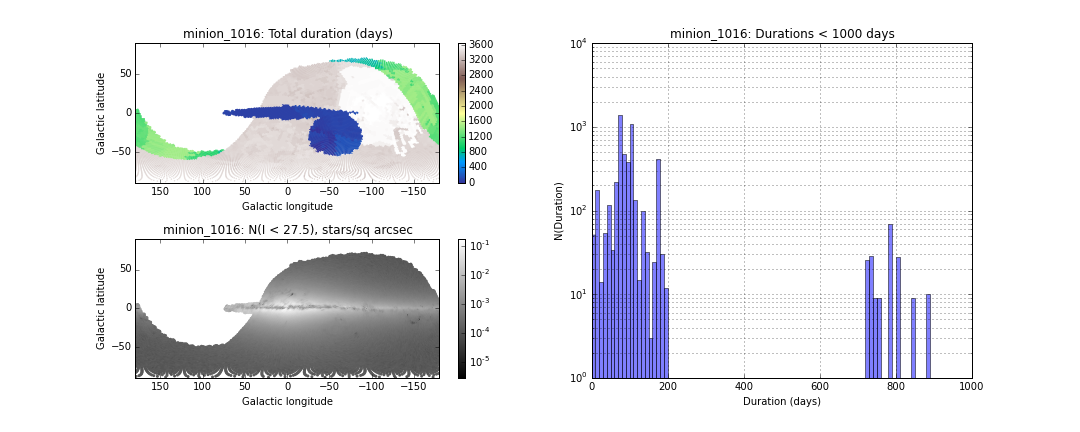
\includegraphics[width=6.0in]{./figs/milkyway/durations_minion_1016.png}
  \caption{The first-order systematics that dominate transient metrics in the Galactic Plane. These panels are plotted for strategy \opsimdbref{db:baseCadence}. {\it Bottom-left:} stars per square arcsecond (at $i < 27.5$). {\it Top-left:} survey duration (defined as the last minus the first MJD for observations in $i$-band). {\it Right:} histogram of durations in $i$-band over the range 0-1000 days. The population below 200 days shows the Plane and South Polar Cap, the population at $\sim 800$~days is the shorter end of the population of Northern Ecliptic observations. Spatial maps are plotted in Galactic co-ordinates.}
\label{fig_durationInGalacticCoords}
\end{figure}

%An important collateral benefit of studies in the plane with an
%LSST-like facility, is improved mapping of the distribution and
%observational effects of the ISM (particularly dust), which is of
%importance to all IR/Optical/UV observational studies. \new{Due to its
%  importance for {\it all} Milky Way Astronomy, a separate Section is
%  devoted to the impact of observing strategy on the utility of LSST
% data to constrain the distribution of interstellar dust in three
%  dimensions (\autoref{sec:MW_Dust}).}

% --------------------------------------------------------------------

\subsection{Target measurements and discoveries}
\label{sec:\secname:MW_Disk_targets}

%Describe the discoveries and measurements you want to make.

%Now, describe their response to the observing strategy. Qualitatively,
%how will the science project be affected by the observing schedule and
%conditions? In broad terms, how would we expect the observing strategy
%to be optimized for this science?

Four Milky Way disk science cases that have complementary dependencies on
observing strategy (e.g. slow intrinsic variability vs fast intrinsic
variability vs no variability) are:

\begin{enumerate}
  \item Quantifying the large quiescent compact binary population via variability;
  \item New insights into the behavior of Novae and the route to Type Ia Superovae;
  \item The next Galactic Supernova;
  \item Measuring population parameters of planets outside the Snow Line with Microlensing;
  %\item A three-dimensional Dust map and improvements in the reddening law
\end{enumerate}

Below we provide more detail on these science cases, including
qualitative discussions of the expected impact of observing
strategy, as these science cases are not discussed in detail elsewhere
(in the LSST Science Book or the \citealt{IvezicEtal2008} summary paper).

%When the figures of merit have been
%computed for these science cases, the results will be summarized in a
%Table in \autoref{sec:\secname:MW_Disk_discussion}.

{\bf 1. Probing quiescent compact binaries via variability:} Of the
millions of stellar-mass black holes formed through the collapse of
massive stars over the lifetime of the Milky Way, only $\sim 20$ have
been dynamically confirmed through spectroscopic measurements
\citep[e.g.,][]{2015arXiv151008869C}.  Many questions central to modern
astrophysics can only be answered by enlarging this sample: which
stars produce neutron stars and which black holes; whether there is a
true gap in mass between neutron stars and black holes; whether
supernova explosions result in large black hole kicks.

There is expected to be a large population of black hole binaries in quiescence
with low X-ray luminosities from $\sim 10^{30}$--$10^{33}$ erg s${-1}$.
Such systems can be identified as optical variables that show unique,
double-humped ellipsoidal variations of typical amplitude $\sim 0.2$
mag due to the tidal deformation of the secondary star, which can be a
giant or main sequence star. In some cases analysis of the light curve
alone can point to a high mass ratio between the components,
suggesting a black hole primary; in other cases the accretion disk
will make a large contribution to the optical light which results in
intrinsic, random, and fast variations in the light curve. The disk
contribution to optical light can change over time, and several years
of data is necessary to properly subtract the accretion disk
contribution in order to properly fit ellipsoidal variations
\citep{2010ApJ...710.1127C}.
The brighter sources will be amenable to spectroscopy
with the current generation of 4-m to 10-m telescopes to dynamically
confirm new black holes; spectroscopy of all candidates should be
possible with the forthcoming generation of large telescopes. Thus,
LSST would trigger a rich variety of observational investigations of
the accretion/outflow process through studies of this large, dark
population.

While we have focused above on black hole binaries, we note that LSST
will, with suitable cadence, allow crucial measurements of the
populations of neutron star and white dwarf binaries. For example, the
total number of compact binaries is presently poorly
understood---Population models of neutron star X-ray binaries diverge
by orders of magnitude, largely due to uncertainties in the common
envelope phase of binary evolution
\citep[e.g.,][]{2003ApJ...597.1036P,2006MNRAS.369.1152K,2015A&A...579A..33V}.
This is poorly constrained but has a large impact on, for example,
LIGO event rates. A simple test case of common envelope evolution is
available in the number of dwarf novae (DNe; accretion disk
instability outbursts around white dwarfs), a population that does not
suffer from some of the complicating factors that neutron star and
black hole binaries do (e.g. supernova kicks).  Theoretical estimates
routinely yield a significantly higher number of DNe than are observed
in the solar neighborhood. Understanding the true specific frequency
of these systems provides a key check on common envelope evolution.
LSST will detect dwarf novae, which last at least several days with
typical amplitudes of 4--6 mag, out to kpc scales. This will allow a
test of not only the number of cataclysmic variables, but also of the
3D distribution within the Galaxy and dependence on metallicity
gradients \citep{2015MNRAS.448.3455B}.

{\it Response to observing strategy:} Since most black hole candidates
have been identified near the plane in the inner Milky Way (68\%~and 92\%
identified within $5^{\circ}$~and $10^{\circ}$~of the Plane, respectively), this science case {\it
    requires} that LSST observe the plane with sufficient cadence to
  detect the $\sim$hundreds of quiescent black-hole binaries by virtue
  of their variability. The natural choice for a survey for
  low-luminosity black hole binaries would be to extend the
  Wide-Fast-Deep survey throughout the Plane in the direction of the
  inner Milky Way. The orbital period of these systems is short (typically $<1$ day), so that a rolling cadence
  for at least parts of the Plane should be considered. For DNe, the cadence of observations
  is critical in obtaining an accurate measure of the population of
  cataclysmic variables, as a long baseline is necessary to recover systems with a low duty cycle, while widely-spaced observations
 would miss short outbursts.

%Describe the discoveries and measurements you want to make.

%Now, describe their response to the observing strategy. Qualitatively,
%how will the science project be affected by the observing schedule and
%conditions? In broad terms, how would we expect the observing strategy
%to be optimized for this science?

{\bf 2. Novae and the route to Type Ia Supernovae:} Only $\sim 15$
novae (explosions on the surfaces of white dwarfs) are discovered in
the Milky Way each year, while observations of external galaxies show
that the rate should be a factor of $\sim 3$ higher
\citep{2014ASPC..490...77S}.
Evidently, we are missing 50--75\% of novae due to their
location in crowded, extinguished regions, where they are not bright
enough to be discovered at the magnitude limits of existing transient
surveys. Fundamental facts about novae are unknown: how much mass is
ejected in typical explosions; whether white dwarfs undergoing novae
typically gain or lose mass; whether the binary companion is important
in shaping the observed properties of nova explosions. Novae can serve
as scaled-down models of supernova explosions that can be tested in
detail, e.g., in the interaction of the explosion with circumstellar
material \citep[e.g.,][]{2015arXiv151007662C}.  Further, since accreting white
dwarfs are prime candidates as progenitors of Type Ia supernovae, only
detailed study of novae can reveal whether particular systems are
increasing toward the Chandrasekhar mass as necessary in this
scenario.

{\it Response to observing strategy:} Most novae occur in the Galactic
Plane and Bulge, and therefore the inclusion of the Plane in a survey
of sufficient cadence to find these events promptly is of paramount
importance for this science. These events will trigger
multi-wavelength follow-up ranging from the radio to X-ray and
$\gamma$-rays; these data are necessary for accurate measurements of
the ejected mass.

{\bf 3. The First Galactic Supernova:} A supernova in the Milky Way
would be among the most important astronomical events of our lifetime,
with enormous impacts on stellar astrophysics, compact objects,
nucleosynthesis, and neutrino and gravitational wave astronomy. The
estimated rate of supernovae (both core-collapse and Type Ia) in the
Milky Way is about 1 per 20--25 years \citep{2013ApJ...778..164A}; hence there
is a 40--50\% chance that this would occur during the 10-year LSST
survey. If fortunate, such an event will be located relatively close
to the Sun and will be an easily observed (perhaps even naked-eye)
event. However, we must be cognizant of the likelihood that the
supernova could go off in the mid-Plane close to the Galactic Center
or on the other side of the Milky Way---both regions covered by
LSST. While any core-collapse event will produce a substantial
neutrino flux, alerting us to its existence, such observations will
not offer precise spatial localization. The models of \citet{2013ApJ...778..164A}
indicate that LSST is the \emph{only} planned facility that
can offer an optical transient alert of nearly all Galactic
supernovae.

{\it Response to observing strategy:} Even if the supernova is not too
faint, LSST will likely be the sole facility with synoptic
observations preceding the explosion, providing essential photometric
data leading up to the event---but only if LSST covers the Plane at a
frequent cadence. Just {\it how} frequent is open to exploration at
present, but the prospect of high-sensitivity observations of the
location of such a supernova {\it before} it takes place are clearly
of enormous scientific value.

% WIC 2016-06-03 - removed following feeback

%A secondary issue is the prospect that
%an easily-observed Milky Way supernova might be too bright for LSST to
%measure precisely with its planned exposure time, with a roughly 82\%
%chance of a core-collapse supernova reaching one or two magnitudes
%brighter than LSST's nominal saturation limit \citep[with a 1/3 chance that
%a ccSN would reach $m_V \sim 5$;][]{2013ApJ...778..164A}. For a Type Ia in
%the Milky Way,
%\citet{2013ApJ...778..164A} estimate $m_{V, max} \lesssim 13.5$~in 92\% of
%cases.

{\bf 4. Population parameters of planets beyond the Snow Line with
  Microlensing:} \citet{gould13}  shows that, LSST could contribute a
highly valuable survey for intra-disk microlensing (in which disk
stars are lensed by other objects in the disk, such as exoplanets,
brown dwarfs, or compact objects). The lower stellar density compared
to past bulge-focused microlensing surveys would be offset by the
larger area covered by LSST. The predicted rate of high magnification
microlensing events that are very sensitive to planets would be $\sim
25$ per year. This survey would be able to detect planets at moderate
distances from their host stars, a regime poorly probed by standard
Doppler and transit techniques. The LSST data alone would not be
sufficient: the detection of a slow ($\sim$ days) timescale increase
in brightness of a disk star would need to trigger intensive
photometric observations from small (1-m to 2-m class) telescopes that
would observe at high cadence for the 1--2 months of the microlensing
event. This would represent an excellent synergy between LSST and the
wider observing community, and would directly take advantage of the
capabilities unique to LSST.

{\it Response to observing strategy:} To catch lensing events as they
start to brighten, with sufficient fidelity to trigger the intensive
follow-up required, the models of \citet{gould13} suggest each field
should be observed once every few nights. With sparser coverage, the
survey would lose sensitivity to microlensing events in
progress. Comparison with a similar sample towards the inner Milky Way
would be highly useful, which would argue for observations of the
entire visible Plane with similar cadence.

Microlensing is also discussed elsewhere in this document, in the
context of exoplanets \autoref{sec:planets}, of the Magellanic Clouds
(\autoref{chp:MCs}), of AGN (\autoref{sec:agn:microlensing}), and of
WFIRST fields towards the Bulge (\autoref{sec:wfirst:microlensing}).
Although the WFIRST discussion in \autoref{sec:wfirst:microlensing}
assumes that Bulge fields will be observed at least at low cadence
($\sim 1$~observation per day) for the first {\it eight} years of the
survey, this is inconsistent with the Baseline strategy that puts all
the Galactic Plane observations into the first few years of the
survey.

% --------------------------------------------------------------------

\subsection{Figures of Merit}
\label{sec:\secname:MW_Disk_metrics}

%Quantifying the response via MAF metrics: definition of the metrics,
%and any derived overall figure of merit.

Here we describe the Figures of Merit (FoMs) we currently intend to implement
and evaluate for the candidate observing strategies of interest. Where
these FoM have already been evaluated, we provide the numerical
results in Table \ref{tab_SummaryMWDisk}. At present, only FoM 3.1 has been
implemented and run for three surveys, with the others in
development. The FoMs are:

\begin{itemize}
  \item FoM 1.1 - Fraction of quiescent black hole binaries detectable through ellipsoidal variability;
  \item FoM 1.2 - Uncertainty on the duty cycle distribution of Dwarf Novae;
  \item FoM 2.1 - Fraction of Novae detected by LSST (specific and total);
  \item FoM 2.2 - Fraction of Novae caught early enough by LSST to schedule followup observations;
  \item FoM 3.1 - Fraction of Galactic supernovae for which LSST would detect variability {\it before} the main Supernova event;
  \item FoM 4.1 - Fraction of accurately-triggered Microlens candidates;
  \item FoM 4.2 - Uncertainty in the mass function of intra-disk microlensed planets.
\end{itemize}

With the exception of FoM 3.1 above, all these Figures of Merit are
likely to be impacted by spatial confusion, as the populations of
interest tend to lie at low Galactic latitudes. Metrics for assessing
the impact of crowding have been developed (e.g. {\tt
  CrowdingMetrics.ipynb} in {\tt maf\_contrib}), and these should be
incorporated into all the FoMs described here. For the present,
however, we note that intrinsic source confusion is not a function of
observing strategy (assuming the confusion limit is well above the
formal limiting magnitude without it). Running the FoMs without
accounting for source confusion isolates the impact of strategy alone
on the science that can be performed, as FoMs can be compared in a
relative sense. Inclusion of crowding will later set the absolute
scale for each FoM.

In these FoMs, ``uncertainty'' can be taken to mean both random and
systematic uncertainty, likely recorded as separate numbers for each
FoM. We anticipate determining the FoMs that record population
parameter-uncertainty in a Monte Carlo sense. This is particularly
relevant for FoMs in which the event rate per pointing may be low
($\lesssim 1$~event per pointing per decade) but not so low that only
1-few events are expected over the whole sky over the lifetime of the
survey (as is the case for FoM 3.1, the First Galactic Supernova). In
very rare-event cases, the FoM can scale with the stellar density and
the recovery fraction of that particular transient, and need only be
evaluated once for the entire survey.

Since (at the time of writing) evaluating a Metric with relaxed SQL
constraints typically takes about 0.5-1.5 hours (on a reasonably
modern laptop), we do not expect to perform Monte Carlo population
simulations initially. In the medium-term, when Monte Carlo
experiments in the target populations are desired, the best strategy
may be to evaluate the run of a particular metric against a parameter
of interest (apparent magnitude, say, which is also expected to lead
to a turnover in the importance of confusion error), and the
investigator's preferred Monte Carlo framework for their population of
interest can interpolate the stored Metric values at the time of
trial-population generation. We have begun investigating the use of
these ``Vector Metrics'' for Figures of Merit, and describe the
anticipated FoMs in these cases below.

{\bf FoM 1.1 - Fraction of quiescent black hole binaries detectable
  through ellipsoidal variability:} Table
  \ref{table:pseudoFOM_1p1} outlines the steps to evaluate FoM
  1.1. Since the lightcurve {\it shape} matters in addition to the
  detection (i.e. we expect LSST data to be used to characterize
  ellipsoidal variations, not just to trigger followup by other
  observatories) the metric choice for detectability should take the
  lightcurve shape into account.

  We envisage two levels to implementing FoM 1.1. In the immediate
  future, the ellipsoidal lightcurve could be characterised as a
  sinusoid, with filter-dependent amplitude to match typical quiescent
  Low Mass X-ray Binaries (qLMXBs) from the literature. The next level
  of sophistication would be to input a more complicated shape that
  captures deviations from pure sine-wave behavior, likely using the {\tt
    TransientAsciiMetric}.

An open question is how best to meaningfully quantify the
  recovery fraction of a population with a wide range in binary
  parameters. However, as an initial FoM, evaluating once for an
  ``average'' population will allow direct comparison between
  observing strategies.

{\it Possible higher-order FoM:} A higher-order FoM for the fraction
of qLMXBs recovered might take the form of the uncertainty on the
population size (or physical population parameter like mass function
slope) derived from a survey under a given observing strategy. One can
imagine summing the ``recovered'' qLMXB population count and comparing
it to that simulated. Some white noise componant of varying strengths
could be added to the light curves to simulate various contributions
of the accretion disk to the continuum light.  Note that the survey
will necessarily be highly incomplete (due to inclination effects,
etc.), it is the likely {\it uncertainty} on the
completeness-correction that would be crucial in this case.

\begin{table}[h]
  \small
  \begin{tabular}{c p{12cm}}
    & {\it FoM 1.1 - Fraction of quiescent black hole binaries (qLMXB) detectable by LSST through ellipsoidal variability} \\
    \hline
  1. & Pick a typical binary mass ratio and separation for $qLMXB$ \\
  2. & Identify typical ellipsoidal variation amplitude and period, for each filter \\
  3a. & {\it Near-term:} Run {\tt periodicStarMetric} to determine the fraction of typical qLMXBs that would be recovered. Or; \\
  3b. & Run a variant of {\tt periodicStarFit.ipynb} that allows the appropriate double-humped lightcurve shape. \\
  4. & {\bf Arrive at FoM 1.1:} Load the result from 4. and sum over the spatial region (to be determined: Galactic Latitude range? Comparison high-latitude clusters?) where the qLMXBs are expected.\\
\hline
    \end{tabular}
 \caption{Description of Figure of Merit 1.1.}
  \label{table:pseudoFOM_1p1}
\end{table}

%Dependencies:
%\begin{itemize}
%  \item Monte Carlo in period, phase and shape parameters (ASCII input?) for va%riables as measured in a particular OpSim run. Likely run Monte Carlo for a rep%resentative number (ten?) of well-chosen orbital periods within the 0.1-5d range;%
%  \item (Since these are short-period objects): the ``PeriodicMetric'' of Lund et al. (2015);
%  \item Will likely need reasonably high-spatial-resolution HEALPIX slices and a prescription for population density as a function of position on-sky (can be analytic).
%\end{itemize}
%Possible higher-order FoM: errors on the population size (mass
%function??) derived from a survey under a given observing
%strategy. Can imagine just adding up the ``recovered'' qLMXB
%population and comparing it to that simulated. Some white noise componant of va%rying strengths could be
%added to the light curves to simulate various contributions of the accretion di%sk to the continuum light.
%Note that the survey will necessarily be highly incomplete (inclination effects, etc.), it
%is the likely {\it uncertainty} on the completeness-correction that
%would be crucial in this case.

{\bf FoM 1.2 - Uncertainty in the duty cycle distribution of Dwarf
  Novae:} Table \ref{table:pseudoFOM_1p2} illustrates a version of
this FoM that could be run in the near future. This FoM could then be
adapted later in a more sophisticated analysis that estimates the
uncertainty in the population recovered (of a Dwarf Nova sub-class of interest,
perhaps). Dwarf Novae are a heterogeneous class; we imagine assigning
an average lightcurve to a population and determining the recovered vs
input duty cycle, under the assumption that the spatial distribution
of recurrent Dwarf Novae is uniform. This isolates the impact of
observing strategy alone due to gaps in coverage. Rather than a full
Monte Carlo simulation in Dwarf Novae populations, initially the
investigator might compute the FoM for a representative range of duty
cycles (since the error on timescale recovery may be expected to scale
with the duty cycle itself).

\begin{table}[h]
  \small
  \begin{tabular}{c p{12cm}}
    & {\it FoM 1.2 - Uncertainty in the Dwarf Nova duty cycle} \\
    \hline
  1. & Pick a typical lightcurve for the Dwarf Nova class of interest; \\
  2. & Assign a duty cycle (and thus typical outburst recurrence timescale); \\
  3. & Run {\tt TransientMetricASCII} using this lightcurve and duty cycle; \\
  4. & Combine the (spatially distributed) results of 3. into a median and formal random uncertainty estimate on the duty cycle estimated from each line of sight; \\
  5. & Compute the offset and its formal error, between the median from 4. and the input duty cycle from 2;\\
  6. & {\bf Arrive at FoM 1.2:} The four numbers from steps 4. and 5. are the characterization of the uncertainty in duty cycle required. \\
\hline
    \end{tabular}
 \caption{Description of Figure of Merit 1.2.}
  \label{table:pseudoFOM_1p2}
\end{table}

{\it Possible higher-order FoM:} The uncertainty in LIGO event rates
due to uncertainties in common envelope evolution, which drives
uncertainties in both LIGO event rates and DN population. While
Advanced LIGO is already starting to place limits on compact object
merger rates \citep[e.g.][]{2016PhRvX...6d1015A}, LSST observations
will provide important electromagnetic constraints on merger rate
results from direct gravitational detection.

%Dependencies:
%\begin{itemize}
%  \item Monte Carlo in distribution of maximum brightness and rise/decay timescale;
%    \item "Triples" without filter constraints (given a prior detection in each filter)- what fraction are recovered?
%    \item Histogram of duty cycle recovery efficiency versus duration of outburst and recurrence time.
%    \item Histogram of recovery efficiency of maximum brightness of dwarf nova versus duration and recurrence time (if assume subsequent outbursts have similar profiles).
%    \end{itemize}

{\bf FoMs 2.1 \& 2.2 - Fraction of Novae characterized by LSST; and the fraction detected early enough to schedule scientifically useful follow-up observations:} Since the set of Novae is so heterogeneous, one can imagine a two-stage process. In the near-future, a single run of {\tt TransientMetricASCII} using some sense of an ``average'' Nova as tracer to enable comparison between observing strategies. We present this in Table \ref{table:pseudoFOM_2p1}, which includes examples for the specific and total fraction of Novae recovered.

In the longer term, a Monte Carlo simulation could be run on a particular class of Novae depending on the parameters of the overall population whose constraints are desired. This latter effort would likely require further development of the Vector Metrics.

\begin{table}[h]
  \small
  \begin{tabular}{c p{12cm}}
    & {\it FoMs 2.1 \& 2.2 - Novae identified from LSST data} \\
    \hline
  1. & Pick a typical lightcurve for the Nova class of interest; \\
  2. & Run {\tt TransientMetricASCII} using this lightcurve; \\
  3. & {\bf Arrive at FoM 2.1a: Specific fraction of Novae discovered:} Sum the result from 2. over the spatial region of interest; \\
  4. & {\bf Arrive at FoM 2.1b:} Multiply the result of 2. by the result of the {\tt Starcounts} metric. Sum this to find the fraction of Novae recovered if their spatial density follows the stellar density in the Milky Way. \\
  \hline
  5. & From the typical lightcurve and a typical follow-up scenario, determine the time interval before outburst peak that would be required to schedule followu-up observations;\\
  6. & Use these to produce appropriate parameters for a transient metric that returns the fraction of events detected; \\
  7. & {\bf Arrive at FoM 2.2:} Sum the result of step 6. over the spatial region of interest.\\
\hline
    \end{tabular}
 \caption{Description of Figures of Merit 2.1. \& 2.2.}
  \label{table:pseudoFOM_2p1}
\end{table}


{\it Possible higher-order metrics:} Uncertainty on the specific rate
of Type Ia supernovae using LSST data taken under various observing
strategies.

%Dependencies:
%\begin{itemize}
%  \item Is the ``Triplets'' metric sufficient (i.e. is this ``just'' a case of supplying the metric the correct $\Delta t$~parameter values)?;
%    \item What is the maximum interval since initial rise that would be acceptable? (Is this a function of waveband for followup?)
%\end{itemize}
%Possible higher-order FoM: error on inferred rate of Type Ia supernovae?

%{\bf FoM 3.1 - Maximum time-interval {\it before} triggering of a SN in the Milky Way that LSST would h%ave taken precursor data.}
%Dependencies:
%\begin{itemize}
%  \item This FoM would probably be very easy to calculate (just estimate the mean time between observat%ions). However the acceptable limits still need thought:
%  \item How many colors are sufficient? Any observations at all before the SN goes off, or would a comp%lete set in all filters be needed to characterize the candidate progenitor?
%    \item What level of variability sensitivity is really needed? Would just an extremely deep image of% the SN field before the event be sufficient?
%\end{itemize}
%{\bf FoM 3.2 - Maximum time-interval {\it after} the SN event for triggering followup.}
%Dependencies:
%\begin{itemize}
%  \item Similar to FoM 3.1.
%    \item Is it important to know the discovery space for LSST? If a
%      supernova at $m_V~15$~goes off, other facilities are likely to
%      spot it...
%\end{itemize}


{\bf FoM 3.1 - Fraction of Galactic supernovae for which LSST would
  detect variability {\it before} the main Supernova event:} We have
implemented a simple FoM for the Galactic Supernova case, using the
parameters of SN2010mc as an example whose pre-SN outburst could be
discovered first by LSST. The FoM is defined as the density-weighted
average fraction of transient events recovered, where the average is
taken over the sight-lines within the simulated strategy:
\begin{equation}
  FoM_{preSN} \equiv \frac{ \sum^{sightlines}_{i} f_{var, i} N_{\ast, i} } {\sum^{sightlines}_{i} N_{\ast, i}}
\label{eqn:def_FOM_3p1}
\end{equation}
Here $f_{var, i}$~is the fraction of transient events that
LSST would detect for observing strategy including the $i$'th
sightline, $N_{\ast,i}$~the number of stars present along the $i$'th
sightline, and the FoM is normalized by the total number of stars
returned by the density model over all sightlines. (For the \OpSim
runs tested here, \opsimdbref{db:baseCadence} and
\opsimdbref{db:opstwoPS} and \opsimdbref{db:NormalGalacticPlane}, the normalization factors differ by $\sim
2\%$.) FoM values are in the range $0.0 \le FoM_{preSN} \le 1.0$.

We assume the Pre-SN variability similar to the pre-SN outburst of
SN2010mc \citep{2013Natur.494...65O}. The pre-SN variability is
modeled as a sawtooth lightcurve (in apparent magnitude). We assume
this transient event will always reach brightness sufficient for LSST
to observe, so opt for a very bright peak apparent magnitude in all
filters. We assume that the probability of a supernova going off is
proportional to the number of stars along a particular line of
sight.

In definition (\ref{eqn:def_FOM_3p1}), a lightly-modified version of
{\tt CountMetric} was used to determine $N_{\ast, i}$~with the output
summed over all sight-lines to produce $N_{\ast}$. Module {\tt
  TransientMetric} was used to determine $f_{var, i}$~for each
sight-line.\footnote{The notebooks used to evaluate this version of
  FoM 3.1 can be found in subdirectory {\tt notebooks} of the
  experimental github repository {\tt lsstScratchWIC}, available at
  this link: \url{https://github.com/willclarkson/lsstScratchWIC}}

% WIC 2016-04-26 - removed the old bullets here since they are
% obsolete now!

{\bf FoM 4.1 - Fraction of accurately-triggered Microlens candidates
  within a spatial region of interest:} Table
  \ref{table:pseudoFOM_4p1} lays out a possible FoM for the fraction
  of microlens candidates that LSST might catch sufficiently early
  that follow-up observations can be planned for other facilties. This
  low-level FoM should be straightforward to compute, for a microlens
  template lightcurve corresponding to some suitable average over the
  regime of interest.

\begin{table}
  \small
  \begin{tabular}{c p{12cm}}
    & {\it FoM 4.1 - Fraction of microlens events triggered from LSST observations} \\
    \hline
  1. & Decide on the typical microlens scenario of particular interest; \\
  2. & Produce a template ASCII lightcurve for this scenario; \\
  3. & Determine the characteristics for a trigger; \\
     & ~~~~ e.g. slow rise to 20\% flux above baseline at 7$\sigma$~significance;\\
     & ~~~~ e.g. must be at most $T$~days after the initial rise to schedule follow-up; \\
  3. & run the metric {\tt transientASCII} on this template; \\
  4. & {\bf Arrive at FoM 4.1:} Sum the fraction of detected candidates from 3. spatially over the region of interest.\\
\hline
    \end{tabular}
 \caption{Description of Figure of Merit 4.1}
  \label{table:pseudoFOM_4p1}
\end{table}

{\bf FoM 4.2 - Uncertainty in the mass function of microlensed planets
  past the Snow Line:} Table \ref{table:pseudoFOM_4p2}
  illustrates a possible FoM for a science case concerning uncertainty
  in the parameters of a particular planetary population of
  interest. As with FoM 4.1, in this scenario LSST is used as the
  initial trigger for follow-up observations by other facilities, but
  the observing strategy imposes uncertainty and bias on the eventual
  derived parameters through its removal of parts of the population
  from further study. The investigator could assume a particular
  uncertainty imposed on the mass determination from follow-up
  observations, but this should be fixed for all evaluations of the
  FoM so that LSST strategies can be compared. Strictly speaking, a
  Monte Carlo simulation over many realizations of the input planetary
  population should probably be run. However, formal errors would
  probably be acceptable in the near-term (i.e. formal errors on the
  determination of mass function parameters that are determined from
  the subset of objects that survive LSST's selection function for a
  particular strategy).

\begin{table}
  \small
  \begin{tabular}{c p{12cm}}
    & {\it FoM 4.2 - Uncertainty in the mass function for planets beyond the Snow Line through Microlensing}\\
    \hline
  1. & Parameterize the mass function of the population of interest;\\
  2. & Parameterize its distribution of lens amplitude and timescale;\\
  3. & Parameterize the scaling of event rate with local stellar density;\\
  4. & Generate a sample population over the sky; \\
     & ~~~ Scaling from 3. might be used in conjunction with {\tt maf\_contrib/starcounts}; \\
  5. & Run the transient-recovery metric for this population; \\
     & ~~~ Choice of metric needs to handle spatially varying lightcurve template; \\
     & ~~~ Or, the time-interval parameters should be allowed to spatially vary; \\
  6. & Determine the population of microlens planets that would have been triggered by LSST. Do not sum, but record the indices of the surviving objects; \\
  7. & Apply typical measurement uncertainty from a likely followup campaign; \\
  8. & Fit the determined mass function from this sample of survivors only; \\
  9. & {\bf Arrive at FoM 4.2:} Find the offset (from input) and formal uncertainty on the mass function parameters.\\
\hline
    \end{tabular}
 \caption{Description of Figure of Merit 4.2}
  \label{table:pseudoFOM_4p2}
\end{table}


%{\bf FoM 5.1 - Errors in derived $E(B-V)$, $n_H$~as a function of
%  location in the Plane.}
%Dependencies:
%\begin{itemize}
%  \item SNR scaling with apparent magnitude
%    \item For the M dwarf based technique, the relation between
%      reddening-invariant index $[Q_{gri}]$~and intrinsic $g-i$~are
%      expressed as polynomials, so expect non-linear relation with
%      photometric error.
%      \item This uses a 5th-order polynomial to describe the
%        $(Q_{gri}, g-i)$~stellar locus for M dwarfs $(g-i > 1.6)$.
%        \item Care must be taken to correctly propagate errors through
%          the various indices used - not trivial with so many choices
%          of flux ratio used.
%          \item Uncertainties in the parameterizations used for e.g. color-$M_V$~relationships.
%            \item The above are all for every location probed on the map.
%\end{itemize}

% --------------------------------------------------------------------

\subsection{OpSim Analysis}
\label{sec:\secname:MW_Disk_analysis}

{\bf FoM 3.1: the First Galactic Supernova:} This FoM is described in
Definition (\ref{eqn:def_FOM_3p1}) of
\autoref{sec:MW_Disk:MW_Disk_metrics}.

{\it Parameters used:} The lightcurve used has the following parameters:
rise slope $-2.4$; time to peak; $20$~days; decline slope: $0.08$; total
transient duration: 80 days. All filters are used in the detections, and
20 evenly-spaced phases are simulated for sensitivity to pathological
cases (parameter nPhaseCheck=20). Peak apparent magnitudes used: $\{
11,9,8,7,6,6\}$~in $\{u,g,r,i,z,y\}$. Then, $f_{var, i}$~is taken as the
``Sawtooth Alert'' quantity returned by {\tt TransientMetric}. For the
stellar density metric, distance limits ($10$pc $\le d \le 80$kpc) are
used to avoid biases in the FoM estimate by the Magellanic Clouds.

{\it \bf Results:} $FoM_{preSN}$(\opsimdbref{db:baseCadence})=0.13,
while
$FoM_{preSN}$(\opsimdbref{db:opstwoPS})=0.83.\footnote{2016-04-25: For
  comparison, when run on 2015-era \OpSim runs \opsimdbname{enigma\_1189}
  (Baseline strategy) and \opsimdbname{ops2\_1092} (PanSTARRS-like strategy)
  the results were 0.251 (Baseline) and 0.852 (PanSTARRS-like
  strategy). So the 2016-era \OpSim runs show a sharper disadvantage
  suffered by the Baseline cadence, than before the update.} This FoM
suggests that \opsimdbref{db:opstwoPS} is the best of the cadences we
have tested thus far. However, it is covers less total area on the sky
(spending no time at all on certain regions of community interest like
the South Polar regions) and thus might be unfairly advantaged
compared to \opsimdbref{db:baseCadence}. Exposures are spread over a
smaller area, thus regions including the inner Plane receive better
coverage than they might under a strategy that meets the needs of all
stakeholders).

A more direct comparison includes the recently-completed (at the time
of writing) \OpSim run \opsimdbref{db:NormalGalacticPlane}, which
covers the same regions on the sky as \opsimdbref{db:baseCadence} but
applies the Wide-Fast-Deep strategy to the inner Galactic Plane. This
survey therefore covers the same regions on the sky as the Baseline
cadence. The stragegy \opsimdbref{db:NormalGalacticPlane} still shows
a strong advantage compared to the Baseline survey, with
$FoM_{preSN}$(\opsimdbref{db:NormalGalacticPlane})=0.73, compared to
0.13 for Baseline cadence. See Table \ref{tab_SummaryMWDisk}. Figure
\ref{f_opSim_GalacticSN} presents a breakdown of this figure of merit
across sightlines, for the three observing strategies considered.

\begin{figure}
\begin{center}
  \includegraphics[width=5.25cm]{./figs/milkyway/galacticSN_SkyMap_Baseline.png}
  \includegraphics[width=5.25cm]{./figs/milkyway/galacticSN_SkyMap_PanSTARRS.png}
  \includegraphics[width=5.25cm]{./figs/milkyway/galacticSN_SkyMap_PlaneWFD.png}
%  \includegraphics[width=6cm]{./figs/milkyway/galacticSN_Histogram_1092.pdf}
%  \includegraphics[width=6cm]{./figs/milkyway/galacticSN_Histogram_1189.pdf}
  \caption{Figure of merit $FoM_{preSN}$~describing LSST's sensitivity
  to any pre-Supernova outburst for the Galactic Supernova science case,
  broken down by sightline. $FoM_{preSN}$~is estimated for
  three \OpSim runs (to-date); \opsimdbref{db:baseCadence} (left; Baseline
  cadence), \opsimdbref{db:opstwoPS} (center; PanSTARRS-like
  strategy), and \opsimdbref{db:NormalGalacticPlane} (which assigns Wide-Fast-Deep cadence to the inner Galactic Plane). The normalizing factors $N_{\ast, total}$ are $3.793 \times 10^{10}$~for both \opsimdbref{db:baseCadence} and \opsimdbref{db:NormalGalacticPlane} (that both strategies have the same $N_\ast$~is not a surprise since both cover the same area) and $3.692\times
  10^{10}$~for \opsimdbref{db:opstwoPS}. The imprint of reduced sampling towards
  the inner plane can be clearly seen for \opsimdbref{db:baseCadence}.
  Notice the difference in color scale between the panels. See \autoref{sec:MW_Disk:MW_Disk_analysis}}
\label{f_opSim_GalacticSN}
\end{center}
\end{figure}


% The Figures of Merit listed above must now be implemented and applied to the OpSim databases.

% The metrics listed above should be carefully compared between our proposed run and the baseline cadence.


% --------------------------------------------------------------------

\subsection{Discussion}
\label{sec:\secname:MW_Disk_discussion}

The Figures of Merit listed above must now be implemented within the
\MAF framework and applied to representative science cases.
See Table \ref{tab_SummaryMWDisk} at the end of this subsection for
initial efforts along these lines. We welcome input and volunteers for
this effort.

Qualitatively, however, we can note immediately that the current
baseline cadence (\opsimdbref{db:baseCadence}) partially excludes the
Galactic Plane from the deep-wide-fast survey and instead adopts a
nominal 30 visits per filter as part of a special proposal - which
also tends to cluster the visits in the inner Plane within the first
few years of the survey. This already seriously compromises the time
baseline (see \autoref{fig_astrom_ByTime_pmError} of
\autoref{sec:MW_Astrometry:MW_Astrometry_OpSim} for a demonstration applied to
proper motions).

Whether the Plane should be observed as a ``special survey'' or as
part of Wide-Fast-Deep, remains an open question that we expect the
Figures of Merit (FoM) to answer when fully implemented. For example,
one can imagine reducing observing time in $u$~(and possibly $g$)
bands towards regions of very high extinction at the lowest galactic
latitudes. The scientific impact of such a strategy (e.g. possibly
lower sensitivity to directly-detected compact objects versus improved
coverage for transients in general) should become clear when
implementation and evaluation of the FoMs described in this Section
are complete.


%We have proposed an OpSim run that includes the Galactic Plane in the
%deep-wide-fast survey:

%\url{https://github.com/LSSTScienceCollaborations/ObservingStrategy/blob/master/opsim/Proposal_GP.md}

\begin{table}
  \begin{tabular}{l|p{6cm}|c|c|c|c|p{5cm}}
    FoM & Brief description & {\rotatebox{90}{\opsimdbref{db:baseCadence}}} & {\rotatebox{90}{\opsimdbref{db:opstwoPS}}} & {\rotatebox{90}{\opsimdbref{db:NormalGalacticPlane}  }} &  {\rotatebox{90}{future run 2}} & Notes \\
    \hline
    1.1 & \footnotesize{LMXB ellipsoidal variations}      & - & - & - & - & - \\
    1.2 & \footnotesize{Uncertainty in DNe duty cycle}   & - & - & - & - &  \footnotesize{LSST as initial trigger} \\
    2.1 & \footnotesize{Fraction of Novae detected}       & - & - & - & - &  - \\
    2.2 & \footnotesize{Fraction of Nova alerts}       & - & - & - & - &  - \\
    3.1 & \footnotesize{Galactic Supernova pre-variability} & 0.13 & {\bf 0.83} & 0.73 & - & \footnotesize{Fraction of SN2010mc-like outbursts that LSST would detect; $FoM_{preSN} = f_{var} \times N_{\ast}$} \\
    4.1 & \footnotesize{Fraction of LSST-triggered microlens candidates} & - & - & - & - & - \\
    4.2 & \footnotesize{Uncertainty in derived planetary mass function} & - & - & - & - & \footnotesize{LSST as initial microlens trigger} \\
%    5.1a & \footnotesize{Median (over sight-lines) of the uncertainty in $E(B-V)$} & - & - & - & - & \footnotesize{(Most useful FoM probably a spatial map of the uncertainty.)} \\
%    5.1b & \footnotesize{Variance (over sight-lines) of the uncertainty in $E(B-V)$} & - & - & - & - & - \\
  \end{tabular}
\caption{Summary of figures-of-merit for the Galactic Disk science cases. The best value of each FoM is indicated in bold. Runs \opsimdbref{db:baseCadence} and \opsimdbref{db:opstwoPS} refer to the Baseline and PanSTARRS-like strategies, respectively. Column \opsimdbref{db:NormalGalacticPlane} refers to a recently-completed \OpSim run that includes the Plane in Wide-Fast-Deep observations. See \autoref{sec:MW_Disk:MW_Disk_analysis}. }
\label{tab_SummaryMWDisk}
\end{table}


%Discussion: what risks have been identified? What suggestions could be
%made to improve this science project's figure of merit, and mitigate
%the identified risks?

% ====================================================================
%
\subsection{Conclusions}


We answer below the ten questions posed in \autoref{sec:intro:evaluation:caseConclusions}.

While the science cases developed thus far all rest on
  variability sensitivity in one way or another, we should point out
  that static science should not be sacrificed completely to
  variability studies. This suggests that any strategy covering the
  inner Milky Way must retain at least a minimum total depth in each
  of the $\left\{u,g,r,i,z,y \right\}$~filters, along all sight-lines, in
  order to constrain stellar effective temperatures, metallicities,
  and interstellar extinction directly from LSST photometry \citep[see
    for example the presentation in][and associated
    papers]{ivezic08}. The implied figure of merit for static science
  is straightforward in principle - simply evaluate the photometric
  depth in each filter at which the confusion limit is reached at the
  required photometric precision - but in practice depends on the
  actual set stellar populations along each line of sight. This figure of
  merit is likely to set the minimum acceptable exposure time in each
  filter in each field, and will require a combination of modeling
  work and experience with existing photometric datasets.

\begin{description}

 \item[Q1:] {\it Does the science case place any constraints on the
 tradeoff between the sky coverage and coadded depth? For example, should
 the sky coverage be maximized (to $\sim$30,000 deg$^2$, as e.g., in
 Pan-STARRS) or the number of detected galaxies (the current baseline
 of 18,000 deg$^2$)?}

 \item[A1:] Figures of Merit addressing this question have been
   specified in this chapter, but implementation and execution are
   still in progress. Co-added depth is less important to this science
   than temporal coverage sufficient to measure the variability (at a
   range of timescales) central to the science cases in this chapter
   section. {\it Qualitatively,} we expect the FoMs will indicate that
   the sky coverage within the inner Disk should be maximized subject
   to the constraint that all fields experience LSST coverage
   throughout the full ten-year survey (a condition currently {\it
     not} satisfied by the current baseline cadence,
   \opsimdbref{db:baseCadence}). This is because some of the important
   transients are relatively rare, and/or the spatial distribution of
   the population within the Milky Way disk is of scientific
   importance. To our knowledge, only two \OpSim runs currently exist
   (\opsimdbref{db:opstwoPS} and \opsimdbref{db:NormalGalacticPlane})
   which subject the populations of interest in this section to
   coverage approaching that of Wide-Fast-Deep. A greater variety of
   strategies of inner-plane coverage is needed to explore any
   tradeoffs between time coverage and spatial coverage within the
   inner Disk. One example might be an \OpSim run with (say) 50\%
   spatial coverage at Wide-Fast-Deep-like levels, the other 50\% at
   coverage similar to the Plane mini-survey in
   \opsimdbref{db:baseCadence}.

 \item[Q2:] {\it Does the science case place any constraints on the
 tradeoff between uniformity of sampling and frequency of  sampling? For
 example, a rolling cadence can provide enhanced sample rates over a part
 of the survey or the entire survey for a designated time at the cost of
 reduced sample rate the rest of the time (while maintaining the nominal
 total visit counts).}

\item[A2:] The frequency of sampling is critical for the science
  cases in this section. Requirement on the uniformity of the sampling
  depends on the timescale of variability and is difficult to project
  without the FoMs being evaluated. A FoM to quantify the relative
  importance of each has been outlined in the chapter, but its
  implementation and execution are still in progress. A greater
  variety of observing strategy simulations that offer
  full-time-baseline coverage of the inner Plane are also needed on
  which to run the FoMs. We require suggestions for \OpSim runs with a
  variety of temporal distributions of exposures within the ten-year
  survey lifetime, towards the inner Plane.

 \item[Q3:] {\it Does the science case place any constraints on the
 tradeoff between the single-visit depth and the number of visits
 (especially in the $u$-band where longer exposures would minimize the
 impact of the readout noise)?}

\item[A3:] This depends strongly on the line of sight,
  especially in $u$-band where reddening reduces sensitivity in any
  individual visit (thus impacting variability-searches for very blue
  objects). In those lines of sight, however, large co-added depth in
  $u$~would still be useful for static population studies. For some
  science cases, single-visit photometric depth provides diminishing
  returns even in the redder filters (for example, once depth
  $i\gtrsim 24$~were reached, going deeper would likely not result in
  finding more dwarf novae, since this depth would already be
  sufficient to find such sources beyond the far side of the
  Bulge). However, \OpSim coverage is still relatively sparse in the
  spatial regions discussed. We suggest augmenting the \OpSim coverage
  towards the inner Milky Way with runs with a variety of u-band
  depths (see for example the discussion of strategies
  \opsimdbref{db:DoubleUbandExptime} and
  \opsimdbref{db:DoubleUbandExptimeSameVisits} in Chapter
  \ref{chp:cadexp}). To-date, sufficient \OpSim coverage to answer
  questions about preferred coverage vs. filter for the inner plane
  simply does not exist.

 \item[Q4:] {\it Does the science case place any constraints on the
 Galactic plane coverage (spatial coverage, temporal sampling, visits per
 band)?}

 \item[A4:] Yes. Galactic plane coverage (in most cases, the inner Plane)
   is crucial to all the science cases in this Section, because the
   populations of interest are not found outside the plane in
   sufficient numbers. In most cases, this coverage must be
   sufficiently spread out in time for discovery through variability
   to be possible over the entire ten-year survey.

 \item[Q5:] {\it Does the science case place any constraints on the
 fraction of observing time allocated to each band?}

\item[A5:] We do not have quantitative answers to this question
  yet since the FoMs are mostly still under development and await a
  sufficient range of \OpSim runs to answer them. {\it Qualitatively,}
  however: LSST will likely be crucial in providing prompt color
  information for the rare-but-important events in the inner plane
  (including unusual or scientifically critical microlensing events
  alerted by LSST or other facilities), so we urge nonzero coverage in
  all six filters. Taking the specific case of outbursts from compact
  objects: having two red filters (e.g. $r-i$) would help tremendously
  in breaking degeneracies between distance and luminosity since the
  spectrum of the outbursts discussed here is typically vega-like (so
  any unusual $r-i$~color should be the result largely of interstellar
  reddening). The minimum observing time allocated to each band is likely to be set by the requirement to retain static science goals such as population dissection \citep[see, e.g.][]{ivezic08}; at the present date, however, figures of merit for static science in the inner plane have not yet been evaluated.
%To be most generally useful for static population
%  studies, such as those constraining reddening, $T_{eff}$~and
%  $[Fe/H]$~photometrically following the manner of the SDSS tomography
%  studies \citep[see, e.g.][and references therein]{ivezic08}, coverage in at
%  least $ugriz$~will be required that affords precise photometry at
%  least down to the confusion limit. We do not as-yet have
%  quantitative limits on what this would mean for the distribution of observing time across filters, however.}

\item[Q6:] {\it Does the science case place any constraints on the cadence for deep drilling fields?}

\item[A6:] The science cases in this chapter do not place any
  constraints on the deep-drilling fields already identified. Were
  deep-drilling-like cadence to be possible for a few fields within
  the inner plane, however, it would be hugely useful. For example, to
  recover ellipsoidal variables at short periods, the shortest gap in
  observations should be $\sim$20 minutes. Not all observations need
  to be so close together, but it is important to have at least a few
  baselines that short in order to reliably recover periods between 80
  minutes and 2 hours, where the majority of CVs (and potentially a
  new population of X-ray faint short period XRB outbursts) should
  be. These considerations also apply to any LSST observational campaign that will complement WFIRST observations of the Bulge (Section \ref{sec:wfirst:microlensing}).

 \item[Q7:] {\it Assuming two visits per night, would the science case
 benefit if they are obtained in the same band or not?}

\item[A7:] Qualitatively, visits in two different filters are weakly preferred. Science cases requiring discrimination of
   the class of object would benefit from color information afforded
   by observing in different filters during the same night, and for
   most of the science cases in this section the variation plays out
   in days rather than hours. However, for a subset of the science
   cases (e.g. ellipsoidal variations of counterparts to eRosita
   sources), observations at the same filter would be preferred. If
   the color variation with phase is smaller than the orbital
   variations, then having the colors could give the best of both
   worlds.

 \item[Q8:] {\it Will the case science benefit from a special cadence
 prescription during commissioning or early in the survey, such as:
 acquiring a full 10-year count of visits for a small area (either in all
 the bands or in a  selected set); a greatly enhanced cadence for a small
 area?}

\item[A8:] No, as long as all fields obtain at least some
  coverage in all filters throughout the full 10-year survey
  lifetime. Our expectation is that a given field will experience
  nonuniform cadence over the ten-year survey, with some intervals of
  high cadence followed by some intervals of low cadence. It would be
  useful for some fields to experience their high-cadence intervals
  during the first year in order to better understand detectability
  and systematics, and to update any population simulations as LSST's
  performance is better constrained.

 \item[Q9:] {\it Does the science case place any constraints on the
 sampling of observing conditions (e.g., seeing, dark sky, airmass),
 possibly as a function of band, etc.?}

\item[A9:] At this stage we do not believe that any special
   conditions are required. The inner plane is somewhat unusual in
   that it will likely be confusion-limited rather than
   sky-limited. Thus better seeing would obviously be better for the
   science, however we do not at this stage have any quantitative
   constraints.

 \item[Q10:] {\it Does the case have science drivers that would require
 real-time exposure time optimization to obtain nearly constant
 single-visit limiting depth?}

\item[A10:] Not as long as the achieved limiting depth is accurately
   understood once observations have been taken. In these
   confusion-limited regions, this question is probably constrained
   more by the performance of the photometry software than by
   real-time observing considerations.

 \end{description}


 % ====================================================================

\navigationbar


% PJM: Perry's content is to be merged with Pat's, in Section 5.6
% % ====================================================================
%+
% SECTION:
%    MW_SFH.tex
%
% CHAPTER:
%    galaxy.tex
%
% ELEVATOR PITCH:
%
%-
% ====================================================================

\section{Star Formation History of the Milky Way}
\def\secname{MW_SFH}\label{sec:\secname}

\credit{pmmcgehee}

\label{sec:\secname:targets}

% This individual section will need to describe the particular
% discoveries and measurements that are being targeted in this section's
% science case. It will be helpful to think of a ``science case" as a
% ``science project" that the authors {\it actually plan to do}. Then,
% the sections can follow the tried and tested format of an observing
% proposal: a brief description of the investigation, with references,
% followed by a technical feasibility piece. This latter part will need
% to be quantified using the MAF framework, via a set of metrics that
% need to be computed for any given observing strategy to quantify its
% impact on the described science case. Ideally, these metrics would be
% combined in a well-motivated figure of merit. The section can conclude
% with a discussion of any risks that have been identified, and how
% these could be mitigated.

LSST gives the opportunity to survey extensive areas
around star formation regions in the Southern hemisphere. Among
others, it would allow to study the Initial Mass Function down to the
sub-stellar limit across different environments. Young stars are
efficiently identified by their variability.

Section 8.10.2 in the LSST Science Book (p298--299) provides a
  thorough scientific motivation for the characterization of young
  stars through variability, including discussion of the observational
  signatures of the diverse physical phenomena driving observed time
  variability. The general observable is strong, irregular flaring
  across the entire $ugrizy$~bandpass of LSST. Flaring can last from
  minutes to years, and at amplitudes from a few tenths to several
  magnitudes.

% WIC - the following para has been removed since it's already present
% verbatim at the end of Section 8.10.2 in the LSST Science Book.

%LSST will increase the sample size for detailed follow-up observations
%due its ability to survey star formations at large heliocentric
%distances and to detect variability in embedded and highly extincted
%young objects that would otherwise be missed in shallower
%surveys. During its operations LSST will also provide statistics on
%the durations of high states, for at least one important tracer
%population (the shorter-duration EXor variables).

% --------------------------------------------------------------------

\subsection{Target measurements and discoveries}
\label{sec:\secname:targets}

The nature of the variability in young stars changes with evolutionary
status. For the youngest stars still undergoing significant mass
accretion, FU Orionis and related outbursts can occur due to
circumstellar disk instabilities. As the natal environment dissipates
and the accretion rates drops, the stars take on a Classical T Tauri
appearance where the variability is primarily due to changes in the
accretion flow and rotational modulation of hot spots resulting from
accretion shocks on the protostellar photosphere. Also present are the
signature of cool spots arising from strong magnetic fields. This cool
spot rotational modulation is responsible for the variability in the
disk-less, and older, weak-line T Tauri stars.

Of particular interest are the FUor and EXor variables, which are
  named after the prototype objects FU Orionis \citep{hartmann96}
  and EX Lupi \citep{herbig01} respectively, and for which
  only a relatively small number of examples are known. In these
  pre-main sequence objects, eruptive outbursts of up to 6 magnitudes
  have been observed, with high state durations from years to
  decades. In addition to triggering follow-up observations, LSST
  should be able to set the first population constraints on the
  duration of high states, particularly for the short end of the
  timescale distribution for these eruptive variables.


% \new{(WIC: Material already in LSST Science Book removed.)}


%{\bf CTTS and WTTS material goes here.}

%Here are the references cited above:\\
%Hartmann \& Kenyon 1996, ARA\&A, 34, 207 \\
%Herbig et al. 2001, PASP, 113, 1547 \\
%Herbig 1977, ApJ, 217, 693 \\
%Aspin et al. 2009, ApJ, 692L, 67 \\
%Hodapp et al. 1996, ApJ, 468, 861 \\
%McGehee et al. 2004, ApJ, 616, 1058 \\


%Describe the discoveries and measurements you want to make.

%Now, describe their response to the observing strategy. Qualitatively,
%how will the science project be affected by the observing schedule and
%conditions? In broad terms, how would we expect the observing strategy
%to be optimized for this science?


% --------------------------------------------------------------------

\subsection{Metrics}
\label{sec:\secname:metrics}

In order to assess the ability of LSST to 1) identify and 2) classify
Young Stellar Objects we need to quantify the variability timescales
and amplitudes of both Class I/II (stars with disks, including
Classical T Tauris) and Class III (Weak-line T Tauris).  Inclusion of
eruptive variables (FUor/EXor) is appropriate as well.

In brief, Weak-line T-Tauris are quasi-periodic with amplitudes of 0.1
to 0.3 mag and periods 1 to $\sim$15 days, so their variability is
comparable to that of $\gamma$ Dor stars. Given the temporal evolution
of cool spots, a period recovery analysis such as shown for RR Lyrae
stars is likely difficult.  The embedded systems and Classical T
Tauris are irregular variables but have been shown to have distinctive
colors due to extinction and the ultraviolet and blue excess arising
from accretion shocks.

\autoref{table:pseudoForExor} shows a possible Figure of Merit for the
recovery by LSST of the distribution of EXor high-state duration in
outburst.


\begin{table}
\small
\begin{tabular}{c p{12cm}}
& {\it Figure of Merit for recovery of EXor high--state duration distribution}\\
\hline
1.  & Produce ASCII lightcurve for eruptive outburst \\
2.  & Initialise large array to store the maps of fraction detected as a function of duration and amplitude. \\
2.  & for {\it duration T} in range \{min, max\}:  \\
3.  & ~~~~ for {\it amplitude A} in range \{min, max\}: \\
4.  & ~~~~~~~~~~ run {\tt mafContrib/transientAsciiMetric} \\
5.  & ~~~~~~~~~~ store the spatial map of the fraction detected for this (A, T) pair \\
6.  & Initialise master arrays to hold the run of duration distribution measurements.\\
7. & Produce distribution of high--state durations and amplitudes from which the simulations will be drawn. \\
8.  & for {\it iDraw} in range \{1, nDraws\}:\\
9.  & ~~~~ construct model population with input duration distribution \\
10.  & ~~~~ Apply the stored metrics from 2-5 to measure fraction recovered \\
11.  & ~~~~ Characterize the duration distribution for this draw \\
12. & ~~~~ Fill the {\it iDraw}'th entry in the master arrays. \\
13. & {\bf FoM 1:} Compute the median and variance of the upper/lower quintiles. \\
14. & {\bf FoM 2:} Evaluate the bias between recovered and input high-state duration. \\
\hline
\end{tabular}
\caption{\new{Steps for Figure of Merit recovering the distribution
  for the duration of EXor high states. See Section \ref{sec:MW_SFH:targets} }}
\label{table:pseudoForExor}
\end{table}


% --------------------------------------------------------------------

%\subsection{OpSim Analysis}
%\label{sec:\secname:analysis}

%OpSim analysis: how good would the default observing strategy be, at
%the time of writing for this science project?

% --------------------------------------------------------------------

\subsection{Discussion}
\label{sec:\secname:discussion}

Galactic star formation regions are largely found at low Galactic
latitudes or within the Gould Belt structure. As such study of young
stars with LSST is closely tied to other science goals concerning the
Milky Way Disk and is subject to the concerns of both crowded field
photometry and the observing cadence along the Milky Way.

The embedded and Classical T Tauri stars also undergo significant and
rapid color changes due to accretion processes. The ability of LSST to
track these variations in color could be limited by the interval
between filter changes.

% ====================================================================
%
% \subsection{Conclusions}
%
% Here we answer the ten questions posed in
% \autoref{sec:intro:evaluation:caseConclusions}:
%
% \begin{description}
%
% \item[Q1:] {\it Does the science case place any constraints on the
% tradeoff between the sky coverage and coadded depth? For example, should
% the sky coverage be maximized (to $\sim$30,000 deg$^2$, as e.g., in
% Pan-STARRS) or the number of detected galaxies (the current baseline but
% with 18,000 deg$^2$)?}
%
% \item[A1:] ...
%
% \item[Q2:] {\it Does the science case place any constraints on the
% tradeoff between uniformity of sampling and frequency of  sampling? For
% example, a rolling cadence can provide enhanced sample rates over a part
% of the survey or the entire survey for a designated time at the cost of
% reduced sample rate the rest of the time (while maintaining the nominal
% total visit counts).}
%
% \item[A2:] ...
%
% \item[Q3:] {\it Does the science case place any constraints on the
% tradeoff between the single-visit depth and the number of visits
% (especially in the $u$-band where longer exposures would minimize the
% impact of the readout noise)?}
%
% \item[A3:] ...
%
% \item[Q4:] {\it Does the science case place any constraints on the
% Galactic plane coverage (spatial coverage, temporal sampling, visits per
% band)?}
%
% \item[A4:] ...
%
% \item[Q5:] {\it Does the science case place any constraints on the
% fraction of observing time allocated to each band?}
%
% \item[A5:] ...
%
% \item[Q6:] {\it Does the science case place any constraints on the
% cadence for deep drilling fields?}
%
% \item[A6:] ...
%
% \item[Q7:] {\it Assuming two visits per night, would the science case
% benefit if they are obtained in the same band or not?}
%
% \item[A7:] ...
%
% \item[Q8:] {\it Will the case science benefit from a special cadence
% prescription during commissioning or early in the survey, such as:
% acquiring a full 10-year count of visits for a small area (either in all
% the bands or in a  selected set); a greatly enhanced cadence for a small
% area?}
%
% \item[A8:] ...
%
% \item[Q9:] {\it Does the science case place any constraints on the
% sampling of observing conditions (e.g., seeing, dark sky, airmass),
% possibly as a function of band, etc.?}
%
% \item[A9:] ...
%
% \item[Q10:] {\it Does the case have science drivers that would require
% real-time exposure time optimization to obtain nearly constant
% single-visit limiting depth?}
%
% \item[A10:] ...
%
% \end{description}

% ====================================================================

\navigationbar


% PJM: moved the following to FutureWork, while the metric(s) is/are being implemented
% % ====================================================================
%+
% SECTION:
%    MW_Dust.tex
%
% CHAPTER:
%    galaxy.tex
%
% ELEVATOR PITCH:
%    Metric suggested - uncertainty and bias in $E(B-V)$~estimates as a
%    function of location on-sky - but not yet implemented.
%-
% ====================================================================

% \section{Dust in the Milky Way}
\subsection{Dust in the Milky Way}
\def\secname{MW_Dust}\label{sec:\secname}

\credit{pmmcgehee}
%,
%\credit{willclarkson}

As discussed in the LSST Science Book (particularly its Section 7.5),
possession of an accurate, three-dimensional dust map is important to
many astrophysical studies. The two most significant all-sky maps
generated in the past two decades are the SFD98 maps based on IRAS
observations, and the recent thermal dust maps derived from Planck
submillimeter data. The angular resolutions of both maps are similar -
between 4 to 6 arcminutes.

Both of the aforementioned maps are strictly two-dimensional and contain
no information about the distribution of dust along the line of sight. A
third dimension can be obtained by analysis of accurate stellar
photometry which constrains both the reddening $E(B-V)$ and extinction
$R_V \equiv A_V/E(B-V)$ towards individual stars. This approach requires
determination of the intrinsic stellar colors and the photometric
parallax of each star in the presence of an unknown amount and law of
extinction. Such maps are necessary to accurately measure the intrinsic
luminosities and colors of both Galactic and extragalactic sources.
Recent work on 3-D maps include the Bayesian analysis method based on
Pan-STARRS--1 (PS1) data \citep{green15} and an alternative technique
using SDSS photometry of M dwarfs (McGehee et al. 2016, in preparation).
However, these studies have so far typically been limited to
heliocentric distances of $\lesssim$4.5 kpc. In the full co-added
survey, LSST will be able to map dust structures out to distances
exceeding 40 kpc, thus revealing a detailed picture of this component of
the Milky Way Galaxy.

While the PS1 3-D dust map is a significant advance, it suggests a
number of major improvements that LSST will be able to
provide. Firstly, the PS1 map covers the region of the sky covered in
their 3$\pi$ survey, and thus excludes a large part of the Galactic
Plane towards the South. Secondly, the PS1 map \citep{2014ApJ...789...15S}
saturates at extinctions $E(B-V) > 1.5$ as their tracer stars fall out
of the survey catalogs fainter than $g\sim 22$, meaning that this
high-fidelity map does not extend uniformly to within a few degrees of
the midplane. Thirdly, this map is currently limited to distances $d
\lesssim 4.5$~kpc. Deep LSST data will allow this map to be extended
to much higher extinctions and larger distances. Owing to the high
extinction and the use of blue filters, this project is less affected
by crowding than other projects requiring photometry in the Plane.

The SDSS approach is complementary, and makes use of reddening-free
colors defined in the SDSS $ugriz$~system by \citet{mcgehee05}.
This approach makes use of M dwarf locus in $(g-r,r-i)$
being nearly perpendicular to the reddening vector in that color-color
space. This allows mapping of a reddening-invariant index to the
intrinsic stellar $g-i$ color and subsequent determination of the
light-of-sight reddening. This approach assumes a set extinction law,
i.e $R_V = 3.1$, in order compute the reddening-invariant index from
the observed $g-r$ and $r-i$ colors. Given the relative faintness of M
dwarfs, this technique is distance limited to $\sim$1 kpc when based
on SDSS data. With its significantly greater survey depth to M-dwarfs,
LSST should revolutionize the use of this technique to probe
Interstellar dust.

% --------------------------------------------------------------------

% \subsection{Target measurements and discoveries}
\subsubsection{Target measurements and discoveries}
\label{sec:\secname:targets}

LSST will be in a unique position to measure the changes in the
observed reddening vector due to $R_V$ variations due to its superb
photometric accuracy.  Both of the dust survey techniques mentioned
above can be used on LSST data, and perhaps other methods will be
developed before the start of survey operations.

When focusing on dust in the ISM (as
opposed to time-domain studies, e.g., dust around star-forming
regions or young stars), the main drivers of feasibility are
coverage of the few degrees around the Plane with sufficient photometric depth
and accuracy. This project is less affected by crowding than other
projects requiring photometry in the Plane owing to its use of blue
filters and the high extinction.  Nonetheless, quantiative estimates of
the expected photometric accuracy in coadded $u$ and $g$ images at low
Galactic latitude are desirable.

Production of a 3-D map of the dust component of the ISM based on LSST
photometry will tell us how much dust is present, what type it is, and
where it is along the line of sight.  The latter concern brings in
issues of how to determine stellar photometric parallaxes ($\mu = m-M$)
under an unknown reddening. The dust maps that are created will consist
of the median and variance of $E(B-V)$ and $R_V$ expressed as functions
of $\mu$ under a suitable binning scheme. We can create simple Figure of
Merit maps that lose the $\mu$ dependency by computing the mean and
variance of the measured variances in $E(B-V)$ and $R_V$ over the $\mu$
bins.

With the possible exception of sightlines towards star formation
regions, studies of interstellar dust are insensitive to the
distribution in time of the visits. In the case of active star formation
regions it is possible that changes in the ISM could be apparent over
the lifetime of the survey. Pushing to fainter magnitudes (which means
observing these fields with better seeing and longer exposures) will be
important, because more stars are required for better statistical
constraints on the model, because more stars are required that lie
behind the dust. In general, the use of broad band photometry requires
attention to the intrinsic SEDs of the background stars in order to
correct for heterochromatic variations in the effective reddening law.

% % --------------------------------------------------------------------
%
% \subsection{Metrics}
% \label{sec:\secname:metrics}
%
% {\bf Metric 1: Uncertainty and bias in $E(B-V)$~estimates as a
%   function of location on-sky.} Dependencies:
%
% \begin{itemize}
%   \item Stellar population throughout the survey %(e.g. Knut / Peter developments; TRILEGAL?);
%   \item Dust map throughout the survey region;
%   \item Scale photometric error predictions for each band from program requirements per exposure;
%   \item Produce formal estimate on the error in extinction and reddening as a function of position on-sky within the survey.
% \end{itemize}
%
%
% % --------------------------------------------------------------------
%
% \subsection{OpSim Analysis}
% \label{sec:\secname:analysis}
%
% Table \ref{tab_SummaryMWDust} summarizes the science Figures of Merit
% for the ISM science cases with LSST.
% % At the present date (April
% % 2016) placeholder rows are given for the FoM's.
%
% \begin{table}
%   \begin{tabular}{l|p{6cm}|c|c|c|c|p{5cm}}
%     FoM & Brief description & {\rotatebox{90}{\opsimdbref{db:baseCadence}}} & {\rotatebox{90}{\opsimdbref{db:opstwoPS}}} & {\rotatebox{90}{\scriptsize{\tt astro\_lsst\_01\_1004} }} &  {\rotatebox{90}{future run 2}} & Notes \\
%     \hline
%     1.1 & \footnotesize{Median (over sight-lines) of the uncertainty in $E(B-V)$} & - & - & - & - & \footnotesize{(Most useful FoM probably a spatial map of the uncertainty.)} \\
%     1.2 & \footnotesize{Variance (over sight-lines) of the uncertainty in $E(B-V)$} & - & - & - & - & - \\
%   \end{tabular}
% \caption{Summary of figures-of-merit for ISM science cases. The best
% value of each FoM is indicated in bold. Runs \opsimdbref{db:baseCadence}
% and \opsimdbref{db:opstwoPS} refer to the Baseline and PanSTARRS-like
% strategies, respectively. Column {\tt astro\_lsst\_01\_1004} refers to a
% recently-completed OpSim run that includes the Plane in Wide-Fast-Deep
% observations. See Section \ref{sec:MW_Disk}. }
% \label{tab_SummaryMWDust}
% \end{table}
%
%
% --------------------------------------------------------------------

%\subsection{Discussion}
%\label{sec:\secname:discussion}

%Discussion: what risks have been identified? What suggestions could be
%made to improve this science project's figure of merit, and mitigate
%the identified risks?

% ====================================================================
%
% \subsection{Conclusions}
%
% Here we answer the ten questions posed in
% \autoref{sec:intro:evaluation:caseConclusions}:
%
% \begin{description}
%
% \item[Q1:] {\it Does the science case place any constraints on the
% tradeoff between the sky coverage and coadded depth? For example, should
% the sky coverage be maximized (to $\sim$30,000 deg$^2$, as e.g., in
% Pan-STARRS) or the number of detected galaxies (the current baseline 
% of 18,000 deg$^2$)?}
%
% \item[A1:] ...
%
% \item[Q2:] {\it Does the science case place any constraints on the
% tradeoff between uniformity of sampling and frequency of  sampling? For
% example, a rolling cadence can provide enhanced sample rates over a part
% of the survey or the entire survey for a designated time at the cost of
% reduced sample rate the rest of the time (while maintaining the nominal
% total visit counts).}
%
% \item[A2:] ...
%
% \item[Q3:] {\it Does the science case place any constraints on the
% tradeoff between the single-visit depth and the number of visits
% (especially in the $u$-band where longer exposures would minimize the
% impact of the readout noise)?}
%
% \item[A3:] ...
%
% \item[Q4:] {\it Does the science case place any constraints on the
% Galactic plane coverage (spatial coverage, temporal sampling, visits per
% band)?}
%
% \item[A4:] ...
%
% \item[Q5:] {\it Does the science case place any constraints on the
% fraction of observing time allocated to each band?}
%
% \item[A5:] ...
%
% \item[Q6:] {\it Does the science case place any constraints on the
% cadence for deep drilling fields?}
%
% \item[A6:] ...
%
% \item[Q7:] {\it Assuming two visits per night, would the science case
% benefit if they are obtained in the same band or not?}
%
% \item[A7:] ...
%
% \item[Q8:] {\it Will the case science benefit from a special cadence
% prescription during commissioning or early in the survey, such as:
% acquiring a full 10-year count of visits for a small area (either in all
% the bands or in a  selected set); a greatly enhanced cadence for a small
% area?}
%
% \item[A8:] ...
%
% \item[Q9:] {\it Does the science case place any constraints on the
% sampling of observing conditions (e.g., seeing, dark sky, airmass),
% possibly as a function of band, etc.?}
%
% \item[A9:] ...
%
% \item[Q10:] {\it Does the case have science drivers that would require
% real-time exposure time optimization to obtain nearly constant
% single-visit limiting depth?}
%
% \item[A10:] ...
%
% \end{description}

% ====================================================================

\navigationbar


% ====================================================================
%+
% SECTION:
%    MW_Astrometry.tex
%
% CHAPTER:
%    galaxy.tex
%
% ELEVATOR PITCH:
%
%-
% ====================================================================

\section{Astrometry with LSST: Positions, Proper Motions, and Parallax}
\def\secname{MW_Astrometry}\label{sec:\secname}

\credit{willclarkson}, \credit{caprastro}, \credit{dgmonet}, \credit{DanaCD}, \credit{jgizis}, \credit{mliu}, \credit{yoachim}

A number of Milky Way science cases of interest to the Astronomical
community will depend critically on the astrometric accuracy LSST will
deliver. While ``astrometry'' is not a science case in the framework
of this white paper, LSST's astrometric performance will be sensitive
to the particular choice of observing strategy.
%While astrometry is not a science case, high astrometric accuracy enables
%a large number of science cases.
Hence, the LSST Observing Strategy needs to be examined for systematic
trends that might limit or even preclude precise measures of
stellar positions, proper motions, parallaxes, and perturbations that
arise from unseen companions.

Tying together the LSST and Gaia optical reference frames will be
critical to many of the science cases discussed here (and in the LSST
Science book), but the final as-delivered performance of Gaia is of
course not yet known. For example, the apparent magnitude range needed
for reference frame tie-in is not yet constrained for crowded fields
(where bright stars will likely form the essential LSST-Gaia reference
frame tracer population), but this will impact the useful LSST
exposure time for these regions, with corresponding observing strategy
implications.

It will be vital for the interaction between LSST and Gaia to be
studied in detail, in terms of astrometry, photometry, spatial
crowding, and instrumental issues, which will be greatly facilitated
by the second Gaia data-release
\citep[e.g.][]{2016AA...595A...1G}. With Gaia-DR2 still in the future
at the time of writing, here we outline some candidate astrometry
science cases, and perform the relative comparison between candidate
observing strategies. As we show, stark differences due to
time-sampling are already apparent, particularly for inner-Plane
regions of the Milky Way.

\autoref{sec:\secname:MW_Astrometry_measurements} highlights two
science cases at opposite scales of distance from the Sun that require
accurate and precise astrometry and/or proper motion
measurements. \autoref{sec:\secname:MW_Astrometry_metrics} presents
Metrics for LSST's astrometric performance, and discusses Figures of
Merit for the two highlighted science cases. These metrics are applied to two example \OpSim runs in
\autoref{sec:\secname:MW_Astrometry_OpSim}. Finally in Section
\ref{sec:\secname:MW_Astrometry_furtherwork}, the work that is still
needed is discussed, both in terms of the Metrics and the Figures of
Merit that depend on them.

%Each of these cases stresses different aspects of the LSST hardware, software,and observing strategies.

%, here we highlight three representative science cases.
%that illustrate the various impacts of the observing strategy might
%be:
%To highlight the
%various astrometric impacts of the strategy, three science cases have
%been chosen for particular attention:

%\subsection{Introduction: Astrometry as a special case}
%\label{sec:\secname:MW_Astrometry_intro}

\subsection{Target Measurements and Discoveries}
\label{sec:\secname:MW_Astrometry_measurements}

%\begin{itemize}
%\item[1.] Identification of Streams in the Galactic Halo using proper motions.
%\item[2.] A complete sample of stars in the solar neighborhood.
%\end{itemize}
%\item The tie between the Radio and Optical realizations of the International Celestial Reference System.
%\item The specific and ensemble agreement between LSST and Gaia parallaxes.

{\bf 1. Identification of Streams in the Galactic Halo Using Proper Motions}

Much of the Milky Way's stellar halo was built by the accretion of smaller galaxies. Given that these galaxies
were generally of low mass, their tidal debris should still form coherent structures in phase space, especially
in the outer Galaxy where dynamical times are long. The identification of these streams would allow
a reconstruction of the accretion history of the Milky Way. Tides also lead to the dissolution of globular clusters,
leaving notably thin streams that serve as sensitive tracers both of the Galactic potential and of the presence of dark
subhalos.

A relatively small number of streams, originating from both dwarfs and globular clusters, have been identified via photometry
of individual stars in large surveys such as SDSS\@. However, only the highest surface brightness structures can be found
in this manner, and it is often difficult to trace the streams over their full extent. LSST will enable streams to be identified
by stellar proper motions, and combined with targeted follow-up spectroscopy, will yield full 6-D position and velocity measurements suitable for dynamical modeling.
Further, it will allow the discovery of tidal debris that is no longer spatially coherent but which can be unambiguously identified in phase space.

Finally, streams and other kinematically-distinct halo substructure
can be identified and characterized by combining proper motions and
photometry in reduced proper-motion diagrams \citep[e.g.,][]{carlin12},
and by analyzing proper-motions of tracers such as
RR Lyrae and giants over large portions of the sky \citep[e.g.,][]{casettidinescu15}.

{\it Response to observing strategy:} Most stars in streams will be main-sequence stars, and the old main sequence turnoff  is located at $r\sim24$ at a distance of 100 kpc.
The nominal LSST proper motion precision at this magnitude is 1 mas yr$^{-1}$, corresponding to about 475 km s$^{-1}$ at this distance. The proper motion
measurements will be better for brighter stars, but in general ensembles of stars will be necessary for accurate measurements. To make accurate proper motion measurements for faint stars, several key components are required. First, a zero point must be established, possibly via background galaxies located in each field. Next, the observations must cover a sufficient range of epochs to reliably detect linear proper motions.

In principle, streams can be detected using proper motions alone, as
kinematically colder populations than the Galactic field through which
they are observed. On the assumption that intrinsic proper motion
dispersion in a stream is negligible compared to the field dispersion,
the faintness limit for proper motion-only detection of streams is set
approximately by the apparent magnitude at which LSST's proper motion
error becomes comparable to or larger than the field proper motion
dispersion. Based on LSST's nominal astrometric performance (as
communicated in the LSST Science Book), this limit will be reached at
$r \sim 22.5$~(Casetti-Dinescu et al. 2017, forthcoming).

However, {\it characterization} of these streams requires their
  identification over their full lengths of many degrees of the sky, for which relative astrometry over small fields will not be
sufficient. Over most of the main-survey area, asbolute proper
  motion calibration may be achieved using the large number of
  background galaxies expected \citep[e.g.][]{IvezicEtal2008} to set
  the proper motion zero point. By using Gaia stars at the
  bright end as absolute proper-motion calibrators we can quantify the
  precision and accuracy of background galaxies as a link to an
  inertial reference system, and thus improve the calibration at the
  faint end of the survey.

Matching LSST's astrometry to the radio International Celestial Reference System (ICRS) - and thus calibrating LSST's absolute astrometry - is highly likely to proceed via the Gaia optical reference frame. Therefore, tying LSST's position to Gaia's final delivered reference frame will be essential. The accuracy with which this tie-in can be achieved, will likely vary spatially and needs further exploration.

Secondary links to the radio ICRS might proceed by matching LSST positions directly to the radio frame traced by background QSOs. These considerations should be developed by the user community, and will include issues including detectable optical or radio structures that degrade the positions or suggest a displacement between the location of the sources of the radio and optical radiation.

{\bf 2. The Most Complete Sample of Stars in the Solar Neighborhood}

The direct solar neighborhood offers our only chance to get make a complete sample of stars, brown dwarfs, and stellar remnants that encompass the entire formation and dynamical history of the Milky Way. While Gaia will offer parallax measurements for perhaps billions of stars, its faint magnitude limit of $G\sim 20$ will limit its measurements of the lowest-mass objects
and remnants to nearby objects, much less than the thin disk scale height of $\sim 300$ pc. For example, Gaia can only measure parallaxes for $0.2 M_{\odot}$ M dwarfs to about 100 pc
and $0.1 M_{\odot}$ M dwarfs to only \emph{10 pc}, showing that Gaia is ill-suited for studies of the coolest dwarfs. By contrast, LSST can measure parallaxes for $> 10^5$ M dwarfs and thousands of L/T brown dwarfs (the coolest Y dwarfs are too faint even for LSST; little contribution is likely here beyond the sample provided by WISE). Gaia will likewise be limited to cool white dwarfs within $\sim 100$ pc with which to estimate the age of the disk, and the thick disk and halo will be out of reach. LSST can directly compare white dwarf luminosity functions to determine precise differential ages for the thin disk, thick disk, and halo.

{\it Response to observing strategy:} Successfully completing this project will require parallax measurements much fainter than possible with Gaia as well as a verification that the LSST and Gaia parallax measurements are consistent in the overlapping magnitude range.

The measurement of stellar parallax puts the substantial constraints on the observing cadence. There are two major issues: the need to sample a wide range of parallax factor (related to time of year), and breaking the correlation between differential color refraction and parallax factor.

``Parallax factors" characterize the ellipse of the star's apparent motion as seen over the course of a year. The shape of the ellipse is given by the Earth's orbit and is not a free parameter in the astrometric solution. The amplitude of the right ascension parallax factor is close to unity while the amplitude of the declination parallax factor is dominated by the sine of ecliptic latitude.
The right ascension parallax factor has maximum amplitude when the star is approximately six hours from the Sun, so the optimum time for parallax observing is when the
star is on the meridian near evening or morning twilight. Atmospheric refraction displaces the star's apparent position in the direction of the zenith by an amount dependent on both the wavelength of the light and the distance to the zenith. Whereas the measured position of star is a function of the total refraction, the measurement of parallax
and proper motion depends on the differences in the refraction as a function of the color of each star and the circumstances of the observations.  This
dependence is called differential color refraction. The combination of parallax factor and differential color refraction leads to two rules: (i) Observations need to cover the widest possible range in parallax
factor, and (ii) The correlation between parallax factor and hour angle in the observations needs to be minimized.

%with respect to the meanmotion of the reference frame.

%The search for faint proper motion stars has two key components.  The first is the need to identify stars that move from the ensemble of other image features that can cause confusion.  For example, a compact group of stars that contains one or more stars of variable brightness can confuse the catalog correlation algorithm.  The other is the need to establish the zero point. For the case of relative astrometry, meaning the measurement of relative positions in an image, the question remains on how to remove the mean motion of the reference frame.  For example, astrometry on certain classes of galaxies might produce a zero point of sufficient accuracy.  This leads to a third constraint on the observing cadence.
% \begin{itemize}
%\item [3)] Observations must cover a sufficient range of epochs so that stars with
%linear or periodic motions can be identified at a high level of confidence.
%\end{itemize}


%\subsection{Sensitivity of parallax measurements to observing strategy}
%\label{sec:\secname:MW_Astrometry_cadence}

%\medskip


\subsection{Metrics and Figures of Merit for LSST's delivered astrometric accuracy}
\label{sec:\secname:MW_Astrometry_metrics}

%\medskip

First we discuss metrics for the observing strategy that affect all of
LSST's astrometric measurements, then discuss figures of merit for the
two science cases. (The three general metrics were identified years
ago and are already in the suite of \MAF utilities, and they should be
reviewed prior to making final decisions. For this reason, in addition
to the Figures of Merit later in the chapter, we present spatial maps
and histograms for the metrics themselves in Section
\ref{sec:\secname:MW_Astrometry_OpSim}, for representative \OpSim
strategies.)

\begin{itemize}
\item[A)] For each LSST field, the parallax factors at each epoch of
observation need to be computed.  The ensemble of these must be checked for
sufficient coverage of the parallactic ellipse.  In particular, the number of
measures with RA parallax factor less than --0.5 and greater than +0.5
needs to be tallied because these carry the most weight in the solution
for the amplitude (parallax).
\item[B)] For each LSST field,
%the hour angle of the observation needs to be
%computed, and
the correlation between hour angle and parallax factor
needs to be examined for significance.  The observing strategy must minimize
the number of fields with this correlation.
\item[C)] The epochs of observation for each field must be checked for a
reasonable coverage over the duration of the survey and to avoid
collections of too many visits during a few short intervals.
\end{itemize}

Within \MAF, metrics A (parallax factor distribution) and B
  (hour angle and parallax correlation) are implemented in a slightly
  different manner from the prescription above. We describe the
  implemented metrics here.

{\it Parallax factor coverage:} This is \MAFmetric{ParallaxCoverageMetric} in \MAF. For
  each pointing, the parallax factor coverage is parameterized as the
  weighted mean radius of arc $\langle l \rangle$~from the center of
  motion due to parallax, scaled to the range $0 \le \langle l \rangle
  \le 1$. Inverse-variance weighting is used both for $\langle l \rangle$~and for the center of motion due to parallax.
%The
%  inverse-variance weighted mean parallax offset is subtracted from
%  the set of parallax offsets for an object at a given location with
%  unit parallax amplitude, and the inverse-variance weighted mean
%  $\langle l \rangle$~of the resulting residuals is returned,
%The reported $\langle l \rangle$~is scaled
%  to the range $0 \le \langle r \rangle \le 1$.
For each measurement,
  the variance used in the weighting is the estimate of the
  (uncrowded) astrometric uncertainty returned by \OpSim for a star of
  specified fiducial magnitude $r$~at the center of the HEALPIX of
  interest. What constitutes a ``good'' value for $\langle l \rangle$~depends on the location
  of the star in ecliptic co-ordinates. Near either ecliptic pole a
  star with uniform parallax coverage would have $\langle l \rangle
  \approx 1.0$~while on the ecliptic uniform coverage would produce
  $\langle l \rangle \approx 0.5$. For any location, $\langle l
  \rangle \approx 0$~would mean all the observations were taken with
  identical parallax factor and therefore any attempt to fit the
  parallax amplitude would be completely degenerate with the object's
  position.

{\it Parallax-Hour angle correlation:} This is \MAF metric \MAFmetric{ParallaxDcrDegenMetric}. At the level of tens
  of milliarcsec, Differential Chromatic Refraction (DCR) shifts the
  apparent location of the star in a color-dependent manner. Depending
  on the hour-angle distribution of observations throughout the year,
  motion due to parallax can become degenerate with motion due to the
  pattern of DCR values sampled. This metric returns the Pearson
  correlation coefficient $\rho$~between the best-fit parallax
  amplitude and DCR amplitude, returning values in the range $-1.0 \le
  \rho \le +1.0$. The range of acceptable values for this metric is
  still under investigation; Monte Carlo simulation by one of us (DGM)
  suggests the parallax error becomes independent of
  $\rho$~(i.e. other effects dominate) for values $|\rho| \lesssim
  0.7$.



For the stream project discussed above, a simple to state (but perhaps complex to implement) figure of merit
is the number of streams that can be discovered in LSST via their proper motions. As a first
attempt, it would be reasonable to assume about 100 halo streams from old, metal-poor dwarf galaxies with
stellar masses $10^5-10^7 M_{\odot}$ distributed as $r^{-3.5}$. The stream widths and internal velocity
dispersions can be set from galaxy scaling relations, and their 3-D velocities consistent with a simple Galactic mass
model at their radii. Setting the stream lengths is more complicated, but should cover a large range from a few to many kpc.
Over a given area, the stream ``S/N" can roughly be taken as the number of stream stars (identified via proper motion, color, and magnitude)
divided by the square root of the number of field stars. For globular clusters, a similar number of streams could be included, but these should have much smaller widths (10s of pc)
and typical masses $10^4-10^5 M_{\odot}$. Eventually it would be desirable to use actual simulated stream parameters taken from cosmological models of the Milky Way (e.g.,
from the Aquarius simulation).

Solar neighborhood projects will be sensitive to the general parallax and proper motion metrics discussed above. More specific science figures of merit are {\it required} at this stage.  For example, the precision of the differential age measurement between the thin disk and halo, which would depend on the number of white dwarfs that can be isolated
from each population.

\subsection{OpSim Analysis}
\label{sec:\secname:MW_Astrometry_OpSim}

Here we present initial analysis of LSST's astrometric
performance. Two example strategies are assessed: the current baseline
strategy, \opsimdbref{db:baseCadence}, and the more recently-evaluated cadence
\opsimdbref{db:NormalGalacticPlane}, which extends the Wide-Fast-Deep
survey to the Galactic Plane (see Section \autoref{sec:cadexp:alternatives}
for more detail on this run).

%the PanSTARRS-like cadence,
%\opsimdbref{db:opstwoPS}, which greater spatial uniformity and
%superior coverage of the Galactic Plane.

\subsubsection{Metrics: Parallax and proper motion precision}

Here we present the expected astrometric performance of LSST as a function of
location on-sky, for two main cuts on the survey strategies:
\begin{itemize}
  \item By time: objects detected in $\{g,r,i,z\}$, after years 1, 2 and 10
    of the survey (Figures \ref{fig_astrom_ByTime_PACoverage} -
    \ref{fig_astrom_ByTime_paError});
\item By filter: objects detected in $\{g,r,i,z\}$, or in $u$ only, or $y$ only, over the full 10 years of the survey (Figures~\ref{fig_astrom_ByFilter_PACoverage} - \ref{fig_astrom_ByFilter_paError}).
\end{itemize}

Astrometric performance for parallax is quantified using the following
metrics:
\begin{itemize}
  \item[1.] Parallax factor coverage (following metric A of \autoref{sec:\secname:MW_Astrometry_metrics}); values farther from 0 are better). See Figures \ref{fig_astrom_ByTime_PACoverage} \&  \ref{fig_astrom_ByFilter_PACoverage};
    \item[2.] Parallax-Hour angle correlation (metric B of \autoref{sec:\secname:MW_Astrometry_metrics}; values closer to 0 are better). See Figures \ref{fig_astrom_ByTime_PADegen} \& \ref{fig_astrom_ByFilter_PADegen};
      \item[3.] Proper motion error, for a star at apparent magnitude 21.0 in the filter specified (this addresses the distribution of measurement epochs, as recommended in Metric C in \autoref{sec:\secname:MW_Astrometry_metrics}; smaller values are better). See Figures \ref{fig_astrom_ByTime_pmError} \& \ref{fig_astrom_ByFilter_pmError};
        \item[4.] Parallax error, for a star at apparent magnitude 21.0 in the filter specified (smaller values are better). See Figures \ref{fig_astrom_ByTime_paError} \& \ref{fig_astrom_ByFilter_paError}.
\end{itemize}

{\it Limitations of the results presented in Figures \ref{fig_astrom_ByTime_PACoverage} to \ref{fig_astrom_ByFilter_paError}.:}
\begin{itemize}
  \item[i.] The spatial maps are clipped at $95\%$~in order to keep
    the color-scale at a sensible range; in some cases this has had
    the side effect of removing parts of the spatial coverage in the
    \opsimdbref{db:baseCadence} maps.

  \item[ii.] This analysis neglected spatial confusion in high-density regions. While this
    confusion would be the same whatever observing strategy was
    chosen, the measurement uncertainties for proper motion and parallax uncertainty
    should be regarded as lower limits.

    \item[iii.] The choice of fiducial apparent magnitude $r = u = y =
      21.0$~is arbitrary. It
      would be informative to repeat the analysis for a range of
      target apparent magnitudes that are better-matched to the
      specific science cases.

      \item[iv.] The comparison between single-filter and $griz$
        detections likely overestimates the measurement precision for
        the $u$-only and $y$-only detections, as an object only
        detected in a single filter may well not be detected in all
        images taken in that filter. While the comparison between
        filter subsets for a given strategy may therefore be highly
        approximate, the comparison between strategies for the same
        filter should be more reliable.

% WIC 2016-06-01 - item below removed, now that we are comparing two strategies with
% similar sky coverage.

%  \item[v.] We have not yet subdivided the samples by a meaningful
%    spatial co-ordinate (galactic latitude would be the obvious
%    choice). A large part of the breadth of the various metric values in
%    \opsimdbref{db:baseCadence} as compared to \opsimdbref{db:opstwoPS} may be
%      due to spatial nonuniformity of the sampling; replotting the
%      histograms coded by galactic latitude would be highly informative in this context.

\end{itemize}

{\it Indications at this date:} Despite these limitations, we note the following:

% WIC 2016-06-01 - updated for comparing wfdPlane to Baseline, not PanSTARRS-1 as was the case.

\begin{itemize}

  \item[I1.] To first order, proper motion and parallax error are dominated by the total time coverage, as might be expected. For some of the mini-survey regions, particularly (but not limited to) the inner-Plane, the baseline strategy \opsimdbref{db:baseCadence} is {\it dramatically} worse for astrometry than the two alternative candidate strategies tested here. When the tendency of \OpSim to cluster mini-surveys within the first year is corrected, detailed comparison of strategies can proceed given the full spread of observing epochs.

  \item[I2.] Taking snapshots of the survey at various stages of completion (Figures \ref{fig_astrom_ByTime_PACoverage} -  \ref{fig_astrom_ByTime_paError}), strategy \opsimdbref{db:NormalGalacticPlane} is not significantly worse than the current baseline strategy \opsimdbref{db:baseCadence};

\item[I3.] For the extremes of object color (objects detected
  only in the bluest or only in the reddest filter), most of the
  astrometry metrics suggest worse performance with additional
  structure in the spatial variation of astrometric performance (see
  Figures \ref{fig_astrom_ByFilter_PACoverage} -
  \ref{fig_astrom_ByFilter_paError}), compared to objects detected in all filters. Further exploration is strongly suggested.

\item[I4.] The two strategies offering enhanced inner-Plane coverage, \opsimdbref{db:NormalGalacticPlane} and \opsimdbref{db:opstwoPS}, do not meaningfully differ from each other purely in terms of delivered astrometric precision.\footnote{However, the absence of the Northern Ecliptic Spur from \opsimdbref{db:opstwoPS} makes it unlikely that this candidate strategy will score highly for Solar System studies.}

\end{itemize}

%% In the current incarnation, these will be big figures on the page. Consider
%% finding a way to summarize them!
\begin{figure}[ht]
  \begin{center}
  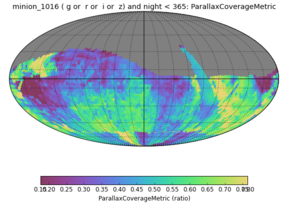
\includegraphics[width=2.0in]{./figs/milkyway/astromPanels/MW_Astrom_paCovge_Baseline_01y_map.png}
  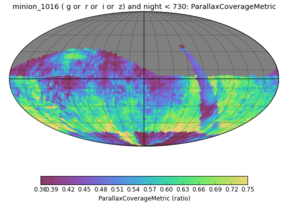
\includegraphics[width=2.0in]{./figs/milkyway/astromPanels/MW_Astrom_paCovge_Baseline_02y_map.png}
  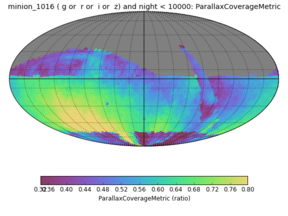
\includegraphics[width=2.0in]{./figs/milkyway/astromPanels/MW_Astrom_paCovge_Baseline_10y_map.png}
  \end{center}
  \begin{center}
  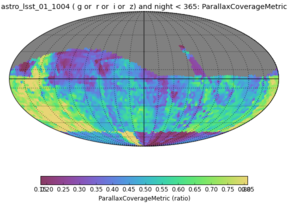
\includegraphics[width=2.0in]{./figs/milkyway/astromPanels/MW_Astrom_paCovge_wfdPlane_01y_map.png}
  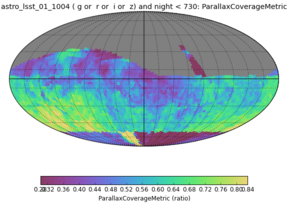
\includegraphics[width=2.0in]{./figs/milkyway/astromPanels/MW_Astrom_paCovge_wfdPlane_02y_map.png}
  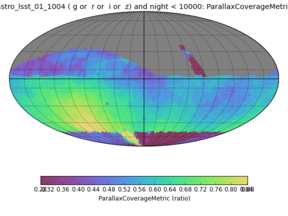
\includegraphics[width=2.0in]{./figs/milkyway/astromPanels/MW_Astrom_paCovge_wfdPlane_10y_map.png}
  \end{center}

  \begin{center}
  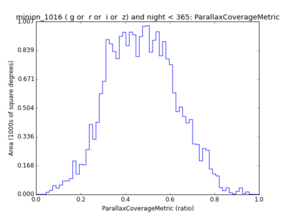
\includegraphics[width=2.0in]{./figs/milkyway/astromPanels/MW_Astrom_paCovge_Baseline_01y_hst.png}
  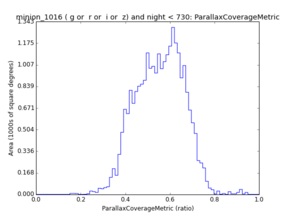
\includegraphics[width=2.0in]{./figs/milkyway/astromPanels/MW_Astrom_paCovge_Baseline_02y_hst.png}
  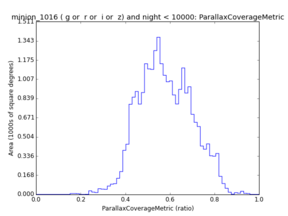
\includegraphics[width=2.0in]{./figs/milkyway/astromPanels/MW_Astrom_paCovge_Baseline_10y_hst.png}
  \end{center}
  \begin{center}
  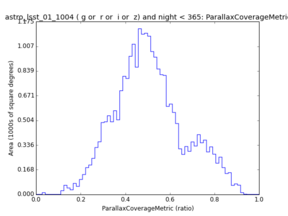
\includegraphics[width=2.0in]{./figs/milkyway/astromPanels/MW_Astrom_paCovge_wfdPlane_01y_hst.png}
  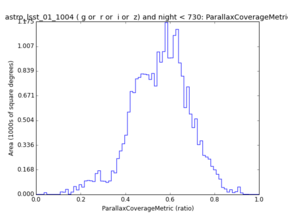
\includegraphics[width=2.0in]{./figs/milkyway/astromPanels/MW_Astrom_paCovge_wfdPlane_02y_hst.png}
  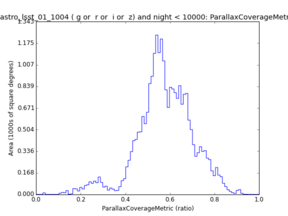
\includegraphics[width=2.0in]{./figs/milkyway/astromPanels/MW_Astrom_paCovge_wfdPlane_10y_hst.png}
  \end{center}
  \caption{Parallax coverage achieved at different epochs within the survey. {\it Top and Third row:} \OpSim run \opsimdbref{db:baseCadence}. {\it Second and bottom row:} \OpSim run \opsimdbref{db:NormalGalacticPlane} (wide-fast-deep extended to much of the inner Plane). Reading left-right, columns represent: {\it Left column:} all observations within the first 365 days of operation; {\it Middle column:} first two years; {\it right column:} the full 10-year survey. Spatial maps are clipped at 95\%, with histogram horizontal limits (0.0 - 1.0).}
  \label{fig_astrom_ByTime_PACoverage}
\end{figure}

\begin{figure}[ht]
  \begin{center}
  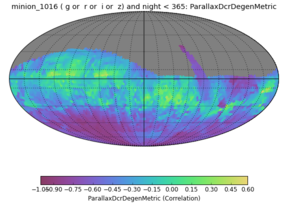
\includegraphics[width=2.0in]{./figs/milkyway/astromPanels/MW_Astrom_paDcrDegen_Baseline_01y_map.png}
  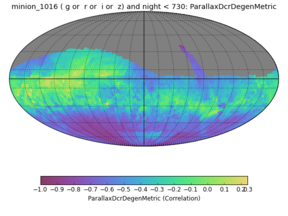
\includegraphics[width=2.0in]{./figs/milkyway/astromPanels/MW_Astrom_paDcrDegen_Baseline_02y_map.png}
  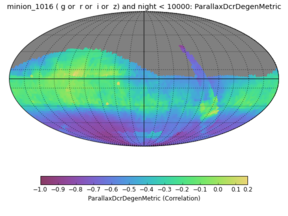
\includegraphics[width=2.0in]{./figs/milkyway/astromPanels/MW_Astrom_paDcrDegen_Baseline_10y_map.png}
  \end{center}
  \begin{center}
  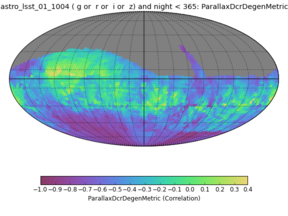
\includegraphics[width=2.0in]{./figs/milkyway/astromPanels/MW_Astrom_paDcrDegen_wfdPlane_01y_map.png}
  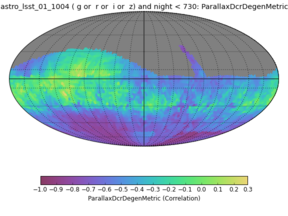
\includegraphics[width=2.0in]{./figs/milkyway/astromPanels/MW_Astrom_paDcrDegen_wfdPlane_02y_map.png}
  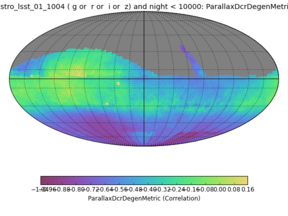
\includegraphics[width=2.0in]{./figs/milkyway/astromPanels/MW_Astrom_paDcrDegen_wfdPlane_10y_map.png}
  \end{center}

  \begin{center}
  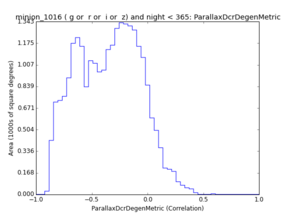
\includegraphics[width=2.0in]{./figs/milkyway/astromPanels/MW_Astrom_paDcrDegen_Baseline_01y_hst.png}
  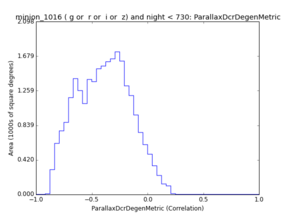
\includegraphics[width=2.0in]{./figs/milkyway/astromPanels/MW_Astrom_paDcrDegen_Baseline_02y_hst.png}
  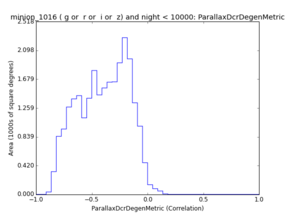
\includegraphics[width=2.0in]{./figs/milkyway/astromPanels/MW_Astrom_paDcrDegen_Baseline_10y_hst.png}
  \end{center}
  \begin{center}
  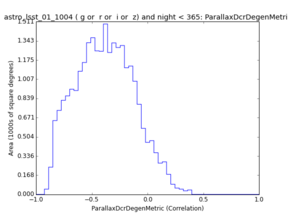
\includegraphics[width=2.0in]{./figs/milkyway/astromPanels/MW_Astrom_paDcrDegen_wfdPlane_01y_hst.png}
  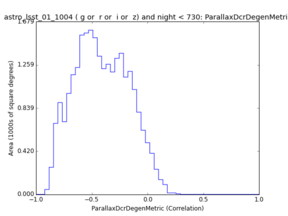
\includegraphics[width=2.0in]{./figs/milkyway/astromPanels/MW_Astrom_paDcrDegen_wfdPlane_02y_hst.png}
  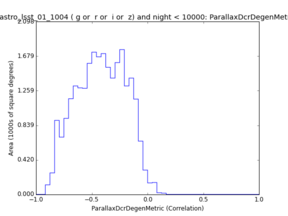
\includegraphics[width=2.0in]{./figs/milkyway/astromPanels/MW_Astrom_paDcrDegen_wfdPlane_10y_hst.png}
  \end{center}
  \caption{Correlation coefficient $\rho$~between parallax and Differential Chromatic Refraction (DCR) up to different epochs within the survey. {\it Top and Third row:} \OpSim run \opsimdbref{db:baseCadence}. {\it Second and bottom row:} \OpSim run \opsimdbref{db:NormalGalacticPlane} (wide-fast-deep extended to much of the inner Plane). Reading left-right, columns represent: {\it Left column:} all observations within the first 365 days of operation; {\it Middle column:} first two years; {\it right column:} the full 10-year survey. Spatial maps are clipped at 95\%, with histogram horizontal scale set to the range $-1.0 \le \rho \le +1.0$.}
  \label{fig_astrom_ByTime_PADegen}
\end{figure}



\begin{figure}[ht]
  \begin{center}
  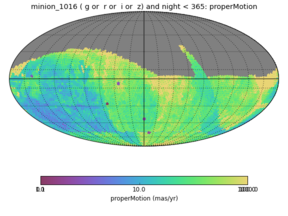
\includegraphics[width=2.0in]{./figs/milkyway/astromPanels/MW_Astrom_pmError_Baseline_01y_map.png}
  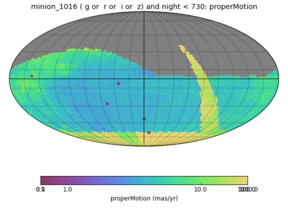
\includegraphics[width=2.0in]{./figs/milkyway/astromPanels/MW_Astrom_pmError_Baseline_02y_map.png}
  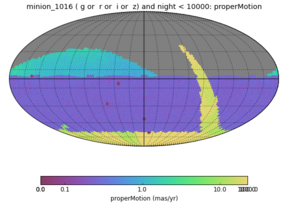
\includegraphics[width=2.0in]{./figs/milkyway/astromPanels/MW_Astrom_pmError_Baseline_10y_map.png}
  \end{center}
  \begin{center}
  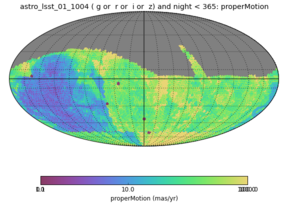
\includegraphics[width=2.0in]{./figs/milkyway/astromPanels/MW_Astrom_pmError_wfdPlane_01y_map.png}
  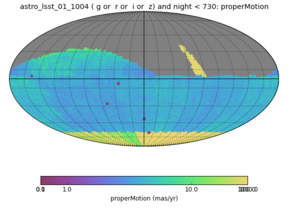
\includegraphics[width=2.0in]{./figs/milkyway/astromPanels/MW_Astrom_pmError_wfdPlane_02y_map.png}
  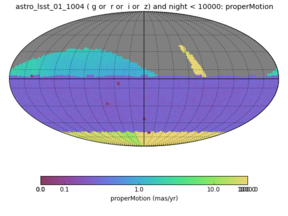
\includegraphics[width=2.0in]{./figs/milkyway/astromPanels/MW_Astrom_pmError_wfdPlane_10y_map.png}
  \end{center}

  \begin{center}
  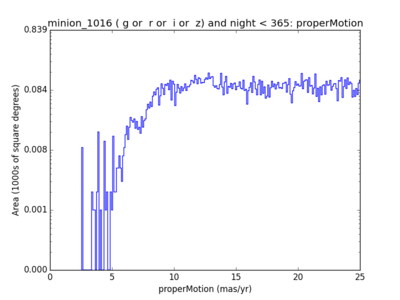
\includegraphics[width=2.0in]{./figs/milkyway/astromPanels/MW_Astrom_pmError_Baseline_01y_hst.png}
  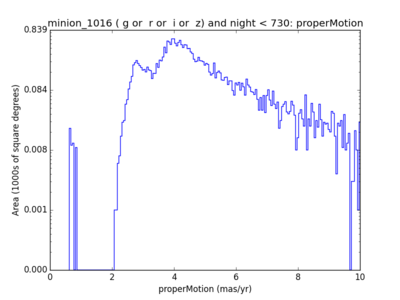
\includegraphics[width=2.0in]{./figs/milkyway/astromPanels/MW_Astrom_pmError_Baseline_02y_hst.png}
  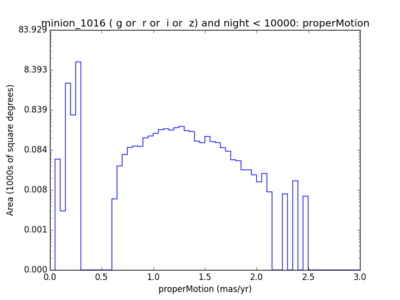
\includegraphics[width=2.0in]{./figs/milkyway/astromPanels/MW_Astrom_pmError_Baseline_10y_hst.png}
  \end{center}
  \begin{center}
  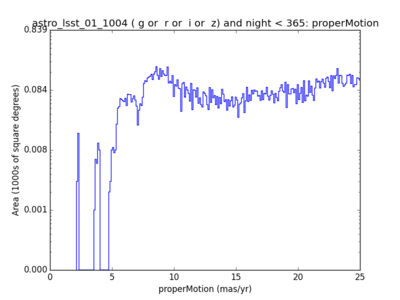
\includegraphics[width=2.0in]{./figs/milkyway/astromPanels/MW_Astrom_pmError_wfdPlane_01y_hst.png}
  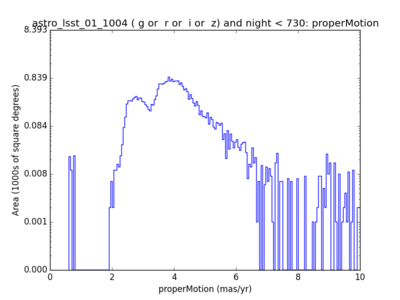
\includegraphics[width=2.0in]{./figs/milkyway/astromPanels/MW_Astrom_pmError_wfdPlane_02y_hst.png}
  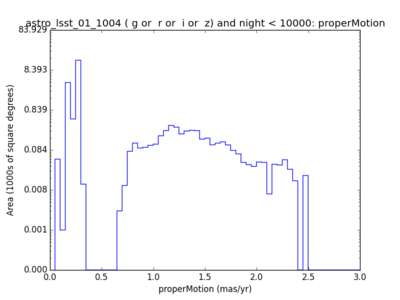
\includegraphics[width=2.0in]{./figs/milkyway/astromPanels/MW_Astrom_pmError_wfdPlane_10y_hst.png}
  \end{center}
  \caption{Proper motion error for a star at $r=21.0$, for different epochs within the survey. Crowding errors are ignored. {\it Top and Third row:} \OpSim run \opsimdbref{db:baseCadence}.  {\it Second and bottom row:} \OpSim run \opsimdbref{db:NormalGalacticPlane} (wide-fast-deep extended to much of the inner Plane). Reading left-right, columns represent: {\it Left column:} all observations within the first 365 days of operation; {\it Middle column:} first two years; {\it right column:} the full 10-year survey. Spatial maps are clipped at 95\% and a log-scale is used for the maps and histograms. Reading left-right, the horizontal upper limits on the histograms are (25, 10, 3.0) mas yr$^{-1}$, respectively. Note that the histograms do not include the full range of values reported in the maps.}
  \label{fig_astrom_ByTime_pmError}
\end{figure}


\begin{figure}[ht]
  \begin{center}
  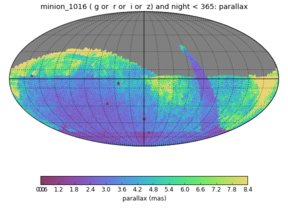
\includegraphics[width=2.0in]{./figs/milkyway/astromPanels/MW_Astrom_paError_Baseline_01y_map.png}
  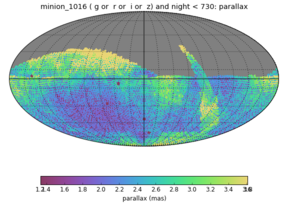
\includegraphics[width=2.0in]{./figs/milkyway/astromPanels/MW_Astrom_paError_Baseline_02y_map.png}
  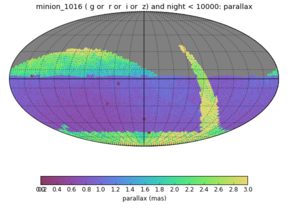
\includegraphics[width=2.0in]{./figs/milkyway/astromPanels/MW_Astrom_paError_Baseline_10y_map.png}
  \end{center}
  \begin{center}
  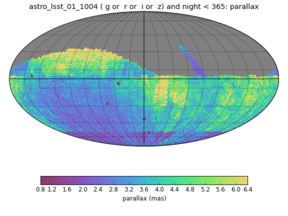
\includegraphics[width=2.0in]{./figs/milkyway/astromPanels/MW_Astrom_paError_wfdPlane_01y_map.png}
  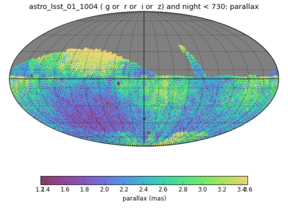
\includegraphics[width=2.0in]{./figs/milkyway/astromPanels/MW_Astrom_paError_wfdPlane_02y_map.png}
  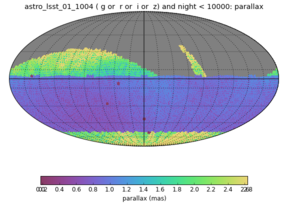
\includegraphics[width=2.0in]{./figs/milkyway/astromPanels/MW_Astrom_paError_wfdPlane_10y_map.png}
  \end{center}

  \begin{center}
  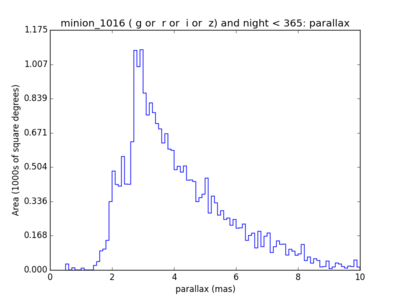
\includegraphics[width=2.0in]{./figs/milkyway/astromPanels/MW_Astrom_paError_Baseline_01y_hst.png}
  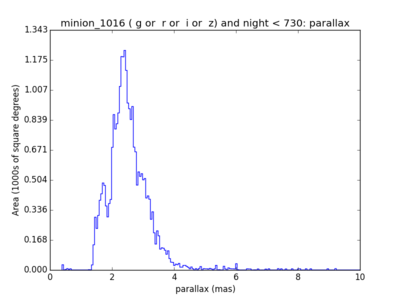
\includegraphics[width=2.0in]{./figs/milkyway/astromPanels/MW_Astrom_paError_Baseline_02y_hst.png}
  \includegraphics[width=2.0in]{./figs/milkyway/astromPanels/MW_Astrom_paError_Baseline_10y_hst.png}
  \end{center}
  \begin{center}
  \includegraphics[width=2.0in]{./figs/milkyway/astromPanels/MW_Astrom_paError_wfdPlane_01y_hst.png}
  \includegraphics[width=2.0in]{./figs/milkyway/astromPanels/MW_Astrom_paError_wfdPlane_02y_hst.png}
  \includegraphics[width=2.0in]{./figs/milkyway/astromPanels/MW_Astrom_paError_wfdPlane_10y_hst.png}
  \end{center}
  \caption{Parallax error for a star at $r=21.0$, for different epochs within the survey. Crowding errors are ignored. {\it Top and Third row:} \OpSim run \opsimdbref{db:baseCadence}. {\it Second and bottom row:} \OpSim run \opsimdbref{db:NormalGalacticPlane} (wide-fast-deep extended to much of the inner Plane). Reading left-right, columns represent: {\it Left column:} all observations within the first 365 days of operation; {\it Middle column:} first two years; {\it right column:} the full 10-year survey. Spatial maps are clipped at 95\%.  Reading left-right, the horizontal upper limits on the histograms are (10, 10, 2.0) mas, respectively.}
  \label{fig_astrom_ByTime_paError}
\end{figure}

%%% Now for the metrics by filter.
\begin{figure}[ht]
  \begin{center}
  \includegraphics[width=2.0in]{./figs/milkyway/astromPanels/MW_Astrom_paCovge_Baseline_u_map.png}
  \includegraphics[width=2.0in]{./figs/milkyway/astromPanels/MW_Astrom_paCovge_Baseline_y_map.png}
  \includegraphics[width=2.0in]{./figs/milkyway/astromPanels/MW_Astrom_paCovge_Baseline_10y_map.png}
  \end{center}
  \begin{center}
  \includegraphics[width=2.0in]{./figs/milkyway/astromPanels/MW_Astrom_paCovge_wfdPlane_u_map.png}
  \includegraphics[width=2.0in]{./figs/milkyway/astromPanels/MW_Astrom_paCovge_wfdPlane_y_map.png}
  \includegraphics[width=2.0in]{./figs/milkyway/astromPanels/MW_Astrom_paCovge_wfdPlane_10y_map.png}
  \end{center}

  \begin{center}
  \includegraphics[width=2.0in]{./figs/milkyway/astromPanels/MW_Astrom_paCovge_Baseline_u_hst.png}
  \includegraphics[width=2.0in]{./figs/milkyway/astromPanels/MW_Astrom_paCovge_Baseline_y_hst.png}
  \includegraphics[width=2.0in]{./figs/milkyway/astromPanels/MW_Astrom_paCovge_Baseline_10y_hst.png}
  \end{center}
  \begin{center}
  \includegraphics[width=2.0in]{./figs/milkyway/astromPanels/MW_Astrom_paCovge_wfdPlane_u_hst.png}
  \includegraphics[width=2.0in]{./figs/milkyway/astromPanels/MW_Astrom_paCovge_wfdPlane_y_hst.png}
  \includegraphics[width=2.0in]{./figs/milkyway/astromPanels/MW_Astrom_paCovge_wfdPlane_10y_hst.png}
  \end{center}
  \caption{Parallax coverage achieved for three extremes of object color, over the full 10-year survey. {\it Top and Third row:} \OpSim run \opsimdbref{db:baseCadence}. {\it Second and bottom row:} \OpSim run \opsimdbref{db:NormalGalacticPlane} (wide-fast-deep extended to much of the inner Plane). Reading left-right, columns represent: {\it Left column:} Objects detected only in the bluest filter; {\it Middle column:} objects detected only in the reddest filter; {\it Right column:} objects detected in all filters. Spatial maps are clipped at 95\%, with histogram horizontal limits (0.0 - 1.0).}
  \label{fig_astrom_ByFilter_PACoverage}
\end{figure}

\begin{figure}[ht]
  \begin{center}
  \includegraphics[width=2.0in]{./figs/milkyway/astromPanels/MW_Astrom_paDcrDegen_Baseline_u_map.png}
  \includegraphics[width=2.0in]{./figs/milkyway/astromPanels/MW_Astrom_paDcrDegen_Baseline_y_map.png}
  \includegraphics[width=2.0in]{./figs/milkyway/astromPanels/MW_Astrom_paDcrDegen_Baseline_10y_map.png}
  \end{center}
  \begin{center}
  \includegraphics[width=2.0in]{./figs/milkyway/astromPanels/MW_Astrom_paDcrDegen_wfdPlane_u_map.png}
  \includegraphics[width=2.0in]{./figs/milkyway/astromPanels/MW_Astrom_paDcrDegen_wfdPlane_y_map.png}
  \includegraphics[width=2.0in]{./figs/milkyway/astromPanels/MW_Astrom_paDcrDegen_wfdPlane_10y_map.png}
  \end{center}

  \begin{center}
  \includegraphics[width=2.0in]{./figs/milkyway/astromPanels/MW_Astrom_paDcrDegen_Baseline_u_hst.png}
  \includegraphics[width=2.0in]{./figs/milkyway/astromPanels/MW_Astrom_paDcrDegen_Baseline_y_hst.png}
  \includegraphics[width=2.0in]{./figs/milkyway/astromPanels/MW_Astrom_paDcrDegen_Baseline_10y_hst.png}
  \end{center}
  \begin{center}
  \includegraphics[width=2.0in]{./figs/milkyway/astromPanels/MW_Astrom_paDcrDegen_wfdPlane_u_hst.png}
  \includegraphics[width=2.0in]{./figs/milkyway/astromPanels/MW_Astrom_paDcrDegen_wfdPlane_y_hst.png}
  \includegraphics[width=2.0in]{./figs/milkyway/astromPanels/MW_Astrom_paDcrDegen_wfdPlane_10y_hst.png}
  \end{center}
  \caption{Correlation coefficient $\rho$~between parallax and Differential Chromatic Refraction (DCR), selecting filters for three extremes of object color, over the full 10-year survey. {\it Top and Third row:} \OpSim run \opsimdbref{db:baseCadence}. {\it Second and bottom row:} \OpSim run \opsimdbref{db:NormalGalacticPlane} (wide-fast-deep extended to much of the inner Plane). Reading left-right, columns represent: {\it Left column:} Objects detected only in the bluest filter; {\it Middle column:} objects detected only in the reddest filter; {\it Right column:} objects detected in all filters. Spatial maps are clipped at 95\%, with histogram horizontal scale set to the range $-1.0 \le \rho \le +1.0$.}
  \label{fig_astrom_ByFilter_PADegen}
\end{figure}

\begin{figure}[ht]
  \begin{center}
  \includegraphics[width=2.0in]{./figs/milkyway/astromPanels/MW_Astrom_pmError_Baseline_u_map.png}
  \includegraphics[width=2.0in]{./figs/milkyway/astromPanels/MW_Astrom_pmError_Baseline_y_map.png}
  \includegraphics[width=2.0in]{./figs/milkyway/astromPanels/MW_Astrom_pmError_Baseline_10y_map.png}
  \end{center}
  \begin{center}
  \includegraphics[width=2.0in]{./figs/milkyway/astromPanels/MW_Astrom_pmError_wfdPlane_u_map.png}
  \includegraphics[width=2.0in]{./figs/milkyway/astromPanels/MW_Astrom_pmError_wfdPlane_y_map.png}
  \includegraphics[width=2.0in]{./figs/milkyway/astromPanels/MW_Astrom_pmError_wfdPlane_10y_map.png}
  \end{center}

  \begin{center}
  \includegraphics[width=2.0in]{./figs/milkyway/astromPanels/MW_Astrom_pmError_Baseline_u_hst.png}
  \includegraphics[width=2.0in]{./figs/milkyway/astromPanels/MW_Astrom_pmError_Baseline_y_hst.png}
  \includegraphics[width=2.0in]{./figs/milkyway/astromPanels/MW_Astrom_pmError_Baseline_10y_hst.png}
  \end{center}
  \begin{center}
  \includegraphics[width=2.0in]{./figs/milkyway/astromPanels/MW_Astrom_pmError_wfdPlane_u_hst.png}
  \includegraphics[width=2.0in]{./figs/milkyway/astromPanels/MW_Astrom_pmError_wfdPlane_y_hst.png}
  \includegraphics[width=2.0in]{./figs/milkyway/astromPanels/MW_Astrom_pmError_wfdPlane_10y_hst.png}
  \end{center}
  \caption{Proper motion error for a star at apparent magnitude $m=21.0$, for three extremes of object color and assessed over the full survey. Crowding errors are ignored. {\it Top and Third row:} \OpSim run \opsimdbref{db:baseCadence}. {\it Second and bottom row:} \OpSim run \opsimdbref{db:NormalGalacticPlane} (wide-fast-deep extended to much of the inner Plane). Reading left-right, columns represent: {\it Left column:} Objects detected only in the bluest filter; the fiducial object has apparent magnitude $u=21.0$; {\it Middle column:} objects detected only in the reddest filter (so $y = 21.0$); {\it Right column:} objects detected in all filters (using $r=21.0$~and a ``flat'' spectrum within \MAF). Spatial maps are clipped at 95\% and a log-scale is used for both the spatial maps and histograms. Reading left-right, the horizontal upper limits on the histograms are (4.0, 4.0, 3.0) mas yr$^{-1}$, respectively. Note that the histograms do not include the full range of values reported in the maps.}
  \label{fig_astrom_ByFilter_pmError}
\end{figure}

\begin{figure}[ht]
  \begin{center}
  \includegraphics[width=2.0in]{./figs/milkyway/astromPanels/MW_Astrom_paError_Baseline_u_map.png}
  \includegraphics[width=2.0in]{./figs/milkyway/astromPanels/MW_Astrom_paError_Baseline_y_map.png}
  \includegraphics[width=2.0in]{./figs/milkyway/astromPanels/MW_Astrom_paError_Baseline_10y_map.png}
  \end{center}
  \begin{center}
  \includegraphics[width=2.0in]{./figs/milkyway/astromPanels/MW_Astrom_paError_wfdPlane_u_map.png}
  \includegraphics[width=2.0in]{./figs/milkyway/astromPanels/MW_Astrom_paError_wfdPlane_y_map.png}
  \includegraphics[width=2.0in]{./figs/milkyway/astromPanels/MW_Astrom_paError_wfdPlane_10y_map.png}
  \end{center}

  \begin{center}
  \includegraphics[width=2.0in]{./figs/milkyway/astromPanels/MW_Astrom_paError_Baseline_u_hst.png}
  \includegraphics[width=2.0in]{./figs/milkyway/astromPanels/MW_Astrom_paError_Baseline_y_hst.png}
  \includegraphics[width=2.0in]{./figs/milkyway/astromPanels/MW_Astrom_paError_Baseline_10y_hst.png}
  \end{center}
  \begin{center}
  \includegraphics[width=2.0in]{./figs/milkyway/astromPanels/MW_Astrom_paError_wfdPlane_u_hst.png}
  \includegraphics[width=2.0in]{./figs/milkyway/astromPanels/MW_Astrom_paError_wfdPlane_y_hst.png}
  \includegraphics[width=2.0in]{./figs/milkyway/astromPanels/MW_Astrom_paError_wfdPlane_10y_hst.png}
  \end{center}
  \caption{Parallax error for a star at apparent magnitude $m=21.0$, for three extremes of object color and assessed over the full survey. Crowding errors are ignored. {\it Top and Third row:} \OpSim run \opsimdbref{db:baseCadence}. {\it Second and bottom row:} \OpSim run \opsimdbref{db:NormalGalacticPlane} (wide-fast-deep extended to much of the inner Plane). Reading left-right, columns represent: {\it Left column:} Objects detected only in the bluest filter; the fiducial object has apparent magnitude $u=21.0$; {\it Middle column:} objects detected only in the reddest filter (so $y = 21.0$); {\it Right column:} objects detected in all filters (using $r=21.0$~and a ``flat'' spectrum within \MAF). Spatial maps are clipped at 95\%. Reading left-right, the horizontal upper limits on the histograms are (10, 10, 2.0) mas, respectively. Note that the histograms do not include the full range of values reported in the maps.}
  \label{fig_astrom_ByFilter_paError}
\end{figure}

\subsubsection{Figures of Merit depending on the Metrics}

Building on the first-order metrics above, this subsection communicates scientific figures of merit for the cases identified in \autoref{sec:\secname:MW_Astrometry_measurements} above.

Table \ref{tab_SummaryMWAstrometry} summarizes the Figures of Merit
(FoMs) for Astrometry science cases. At the time of writing, FoMs have
been implemented to summarize the random uncertainty in proper motion
and parallax, for two regions experiencing extreme values of these
quantities: the inner Plane (conservatively defined in this section as
$|b| \lesssim 7^o$~and $|l| \lesssim 80^o$), and the main survey
(excluding the inner plane and the Southern Polar region, taken
here as $\delta_{2000.0} < -60.0^o$). Figure
\ref{fig_astrom_RegionSelKey} illustrates these selection-regions on
the sky. These form FoM 1.1-1.4, and have to-date been run for the
\OpSim runs \opsimdbref{db:baseCadence} (Baseline cadence),
\opsimdbref{db:opstwoPS} (similar to PanSTARRS-1), and the
recently-completed \opsimdbref{db:NormalGalacticPlane} (which applies
Wide-Fast-Deep cadence to much of the inner Galactic Plane).

From the point of view of parallax and proper motion, the latter two
strategies do not negatively impact the non-plane regions, but they
{\it substantially} improve the sampling for proper motions and
parallax (again, neglecting the effects of spatial crowding).

FoM 1.5 in Table \ref{tab_SummaryMWAstrometry} reports the total number of fields with Parallax/Hour-angle correlation $|\rho| < 0.7$.

At the time of writing, FoMs 2-5 in Table
\ref{tab_SummaryMWAstrometry} are still at the specification stage,
and are described in Section
\ref{sec:\secname:MW_Astrometry_furtherwork}.

%%%% Figures used as ``key'' for the astrometry FoMs:

\begin{figure}[h]
  \begin{center}
    \includegraphics[width=2.0in]{./figs/milkyway/astromPanels/MW_Astrom_FoM_properMotion_minion_1016_all_skymap.png}
  \includegraphics[width=2.0in]{./figs/milkyway/astromPanels/MW_Astrom_FoM_properMotion_minion_1016_plane_skymap.png}
  \includegraphics[width=2.0in]{./figs/milkyway/astromPanels/MW_Astrom_FoM_properMotion_minion_1016_nonPlane_skymap.png}
    \end{center}
  \caption{Selection regions for the Astrometry Figures of Merit (FoMs) 1.1-1.4. Figures of Merit 1.1 and 1.3 refer to the ``main survey'' region shown in the middle panel (which for the FoM also avoids the region of the South Galactic Pole). The right panel shows the inner Plane region to which FoMs 1.2 \& 1.4 refer. The left-hand panel shows the entire survey region for reference. This example shows run \opsimdbref{db:baseCadence}. See Table \ref{tab_SummaryMWAstrometry} and Section \ref{sec:\secname:MW_Astrometry_metrics}.}
  \label{fig_astrom_RegionSelKey}
\end{figure}

\subsection{Topics that will need to be addressed}
\label{sec:\secname:MW_Astrometry_furtherwork}

Here we present suggestions for further work, first on figures of
merit for the science cases, and then on additional Metrics for LSST's
astrometric performance.

\subsubsection{Further work on science Figures of Merit}
%\medskip

At the time of writing, the Figures of Merit for both the highlighted
Science cases need to be implemented and applied to \OpSim output,
preferably in a format that can be summarized in a single Table in
this section. These figures of merit are discussed above in Section
\ref{sec:\secname:MW_Astrometry_metrics} (particularly for the Halo
Streams science project). Figures of merit for the two science cases
might be:
\begin{itemize}
  \item[1.] Number of streams that LSST can discover via their proper motions;
\item[2.] Uncertainty and bias in the thin and thick disk differential age measurement when using white dwarfs from each population as tracers.
\end{itemize}

Given the diversity of science cases that use local Solar Neighborhood
populations as tracers, it may be advantageous to subdivide the Solar
Neighborhood projects into further figures of merit. Two further example
figures of merit might then be:
\begin{itemize}
  \item[3.] Uncertainty and bias in the Brown Dwarf mass function using Solar Neighborhood tracers;
   \item[4.] Uncertainty and bias in the thickness in the main sequence of M-dwarfs within 25pc from the Sun, once variability has been characterized and removed.
\end{itemize}

%%%% SUMMARY TABLE FOR THIS SECTION

\begin{table}
  \begin{tabular}{l|p{4.8cm}|p{1.1cm}|p{1.1cm}|p{1.1cm}|c|p{3.5cm}}
    FoM & Brief description & {\rotatebox{90}{\opsimdbref{db:baseCadence} }} & {\rotatebox{90}{\opsimdbref{db:opstwoPS} }} & {\rotatebox{90}{\opsimdbref{db:NormalGalacticPlane}   }} &  {\rotatebox{90}{future run 2}} & Notes \\
    \hline
    1.1 & \footnotesize{Median parallax error at $r=21$ (main survey)}      & 0.69  & 0.72 & 0.69 & - &
%\footnotesize{Summarize the presentation in Figures \ref{fig_astrom_ByTime_PACoverage}-\ref{fig_astrom_ByFilter_paError} }
\footnotesize{See region definitions in Figure \ref{fig_astrom_RegionSelKey}.}
\\
    1.2. & \footnotesize{Median parallax error at $r=21$ (plane)}   & 2.68 & {\bf 0.91} & {\bf 0.89} & - &
\footnotesize{Smaller values are better.}\\
    1.3. & \footnotesize{Median proper motion error at $r=21$ (main survey)}  & 0.19 & 0.19 & 0.19 & - &
%\footnotesize{Take median of Figure \ref{fig_astrom_ByTime_pmError} over the ``plane'' region.}
\\
    1.4. & \footnotesize{Median proper motion error at $r=21$ (plane)} & 16.7
%$^\dagger$
& {\bf 0.26} & {\bf 0.25} & - &
%\footnotesize{$^\dagger$no, this is not a typo.}
\\
1.5. & \footnotesize{Fields with Parallax-DCR correlation coefficient $\rho \ge 0.7$~/ total fields} & \footnotesize{ \bf{3486} / \bf {31116} } & \footnotesize{3586 / 30107} & \footnotesize{3690 / 31116} & - & \footnotesize{Smaller is better. Value reported after full 10 years of survey for $griz$~detections.}  \\
    \hline
    2.1. & \footnotesize{Number of streams LSST can discover via proper motions} & - & - & - & - &  - \\
    3.1. & \footnotesize{Uncertainty and bias in thin- and thick-disk differential age measurement via white dwarfs} & - & - & - & - &  - \\
    4.1. & \footnotesize{Uncertainty and bias in brown dwarf mass function from the Solar Neighborhood}  & - & - & - & - & \footnotesize{Using astrometry metrics for objects detected only in the reddest filter(s)} \\
    4.2. & \footnotesize{Uncertainty and bias in white dwarf mass function from the Solar Neighborhood}  & - & - & - & - & \footnotesize{Using astrometry metrics for objects detected only in the bluest filter(s)} \\
    5.1. & \footnotesize{Uncertainty and bias in Solar Neighborhood M-dwarf thickness on the MS}  & - & - & - & - &  - \\
\end{tabular}
\caption{Summary of Figures of Merit for the Milky Way Astrometry science cases. The best value of each FoM is indicated in bold. Runs \opsimdbref{db:baseCadence} and \opsimdbref{db:opstwoPS} refer to the Baseline and PanSTARRS-like strategies, respectively. Column \opsimdbref{db:NormalGalacticPlane} refers to a recently-completed \OpSim run that includes the Plane in Wide-Fast-Deep observations. See \autoref{sec:MW_Astrometry}.}
\label{tab_SummaryMWAstrometry}
\end{table}


%%%% SUMMARY TABLE FINISHES HERE


\subsubsection{Further work on Astrometry Metrics}

The MAF metrics presented in Sections \ref{sec:\secname:MW_Astrometry_OpSim} and \ref{sec:\secname:MW_Astrometry_metrics} are only part of the
study of LSST's predicted astrometric performance.  Detailed simulations
and studies need to be done in many other areas as part of the
prediction and verification of LSST's astrometric performance.  Among
the most important are the following.
\begin{itemize}
\item How well do galaxies perform as astrometric reference objects? Are certain shapes or colors better than others? What is the
surface density of ``good" astrometric reference galaxies as a function of filter?
% 2017-06-03 commented out
%\item How well can we identify optically point-like QSOs that will be useful in matching the optical reference frame to the ICRS?
%\item Given the LSST exposure time, site, and physical characteristics, how can we mitigate the limitations on astrometric accuracy imposed by the seeing and local atmospheric turbulence?
\item How does the astrometric performance depend on stellar density? If there are fields in which photometry is only possible via difference imaging, what are the limitations
on astrometry in these fields?
%\item What tools do we need to compare the general and specific agreement between the {\it Gaia} results and the LSST results?
\item Does the ``brighter-wider" effect in the deep-depletion CCDs introduce a magnitude term into the centroid positions?

\item Deep-driling fields will likely be essential to fully understand LSST's astrometric behavior over the entire survey. How should Deep-Drilling fields be specified to fully characterize LSST's delivered astrometric performance?

\end{itemize}

% ====================================================================

\subsection{Conclusions}

Here we answer the ten questions posed in
\autoref{sec:intro:evaluation:caseConclusions}:

\begin{description}

\item[Q1:] {\it Does the science case place any constraints on the
tradeoff between the sky coverage and coadded depth? For example, should
the sky coverage be maximized (to $\sim$30,000 deg$^2$, as e.g., in
Pan-STARRS) or the number of detected galaxies (the current baseline
of 18,000 deg$^2$)?}

\item[A1:] We do expect tradeoffs between depth and sky
  coverage, but we do not yet have the FoM evaluations to set
  quantitative constraints. For example, we expect some combination of
  depth and survey volume would optimize the completeness to objects
  among the populations in the Solar Neighborhood. More generally,
  perhaps, in fields away from the galactic mid-plane, the
  lengthscales over which the proper motion zeropoints can be
  accurately constrained will depend on the spatial density of
  well-measured background galaxies (finer lengthscale corresponding
  to greater co-added depth). The depth must therefore be sufficient
  to sample enough of these galaxies to constrain variations of
  astrometric zeropoint on lengthscales at least as fine as those
  imposed by the LSST system itself (or the atmosphere, whichever is
  finer). We anticipate that this tradeoff can be informed by
  simulation under a set of assumptions for these variations.

\item[Q2:] {\it Does the science case place any constraints on the
tradeoff between uniformity of sampling and frequency of  sampling? For
example, a rolling cadence can provide enhanced sample rates over a part
of the survey or the entire survey for a designated time at the cost of
reduced sample rate the rest of the time (while maintaining the nominal
total visit counts).}

\item[A2:] Yes, although for astrometry the language of these
  constraints is slightly different. The parallactic ellipse must be
  sufficiently covered, the correlation between hour angle and
  parallax factor must be minimized, and the visits must be
  sufficiently distributed (both within a year and over the ten-year
  time baseline) to produce the best precision in both proper motion and parallax. See Section \ref{sec:MW_Astrometry:MW_Astrometry_metrics}.

\item[Q3:] {\it Does the science case place any constraints on the
tradeoff between the single-visit depth and the number of visits
(especially in the $u$-band where longer exposures would minimize the
impact of the readout noise)?}

\item[A3:] More visits at the standard exposure time are
  generally preferred to a few visits with longer exposures, in order
  to achieve as broad a temporal coverage as possible (see Section
  \ref{sec:MW_Astrometry:MW_Astrometry_metrics}). The $u$-band itself
  is likely to be of limited use for astrometry (except possibly for
  extremely blue objects with little signal in any of the other
  filters) due to differential chromatic refraction (DCR), however of
  course $u$-band will still be useful for photometric constraints.

\item[Q4:] {\it Does the science case place any constraints on the
Galactic plane coverage (spatial coverage, temporal sampling, visits per
band)?}

\item[A4:] Not for the example of detecting Galactic Halo
  streams via proper motions (Section
  \ref{sec:MW_Astrometry:MW_Astrometry_measurements}). For the Solar
  Neighborhood populations, avoiding the inner Galactic mid-plane
  would obviously reduce the completeness of the census of nearby
  objects with parallax determinations due to the reduction in total
  area surveyed. However, this reduction may be incremental rather
  than serious. The impact of an inner-plane zone of avoidance on the
  recovery of the parameters describing these constituent populations
  has not yet been evaluated. Of course, this all changes for
  astrometry of objects of interest that lie in the inner plane (see
  also Section \ref{sec:MW_Disk}), where (for example) the reduced
  proper motion will be a useful diagnostic. At present, however, the
  performance of the LSST software stack towards crowded fields is
  as-yet unknown - as is the performance of Gaia in these regions. As this performance becomes better understood, it
  will be possible to quantitatively compare strategies for astrometry
  towards the inner plane.

\item[Q5:] {\it Does the science case place any constraints on the
fraction of observing time allocated to each band?}

\item[A5:] Yes, but indirectly through the requirement to
  measure all the populations of interest in the Solar
  Neighborhood. Making the assumption that this science case requires
  parallax measurements for extremely blue objects as well as
  extremely red objects, which might each be measurable only in a
  single very red or blue filter, would suggest at a minimum that the
  coverage considerations of Section
  \ref{sec:MW_Astrometry:MW_Astrometry_metrics} be applied to
  observations in $u$~and $Y$ filters separately, as well as at least
  one mid-range filter. However the quantitative impact on population
  recovery from various filter-distributions has yet to be assessed at
  this date. Further work is needed to determine if the increased
  sensitivity of $u$-band astrometry to DCR relative to $g$-band would
  prevent its use for astrometry.

\item[Q6:] {\it Does the science case place any constraints on the
cadence for deep drilling fields?}

\item[A6:] The deep-drilling fields will provide essential characterization of LSST's delivered astrometric performance, providing at least a sanity check on the characterization of astrometric accuracy for {\it all} observed fields. The observational design of the deep-drilling fields needs to be carefully considered in terms of their utility for calibrating the non-deep-drilling fields, as well as in terms of maximizing the astrometric precision of the deep-drilling fields in their own right (for which the considerations of Section \ref{sec:MW_Astrometry:MW_Astrometry_metrics} will apply).

%If precision astrometry is desired for the deep drilling fields, then the considerations of Section \ref{sec:MW_Astrometry:MW_Astrometry_metrics} apply to those fields as well.

\item[Q7:] {\it Assuming two visits per night, would the science case
benefit if they are obtained in the same band or not?}

\item[A7:] While detailed investigation is still pending, we
  expect that using different filters within the same night would be
  preferred to allow better constraint of DCR effects. Doing different
  filters on the same night might reduce the number of free parameters
  (like seeing and parallax factor) and give more pairs for direct
  filter-A vs. filter-B astrometry.

\item[Q8:] {\it Will the case science benefit from a special cadence
prescription during commissioning or early in the survey, such as:
acquiring a full 10-year count of visits for a small area (either in all
the bands or in a  selected set); a greatly enhanced cadence for a small
area?}

\item[A8:] It is vital for astrometry that at least a few fields
  be observed with both sufficient parallax factor coverage and
  sufficient number of visits, early in the survey, to demonstrate
  parallax precision specified in the Science Requirements
  Document. In these fields, sufficient exposures must be reserved for
  the entire 10-year survey baseline so that proper motion precision
  is not too badly compromised in these fields. This combination of
  factors may require dedicated commissioning observations of these
  fields in addition to the 10-year survey operations. In addition,
  however, at least a few fields must be observed at a variety of
  values of single-visit achieved depth, and FWHM, in order to
  constrain the degree to which FWHM will actually predict the
  achieved astrometric precision (see also the answer to Q10
  below). This second set of requirements may also be best served by
  dedicated commissioning observations.

\item[Q9:] {\it Does the science case place any constraints on the
sampling of observing conditions (e.g., seeing, dark sky, airmass),
possibly as a function of band, etc.?}

\item[A9:] The observations need to be planned in such a way
  that the correlation between parallax and hour-angle is minimized,
  to avoid deneracies between the motion due to atmospheric refraction and the motion that is sought due to parallax. See
  Section \ref{sec:MW_Astrometry:MW_Astrometry_metrics}.

\item[Q10:] {\it Does the case have science drivers that would require
real-time exposure time optimization to obtain nearly constant
single-visit limiting depth?}

\item[A10:] While optimization on an exposure-to-exposure basis
  is perhaps unlikely, {\it selection} between observations in
  response to conditions (on a timescale of perhaps 10 minutes) will
  be crucial to maximize achieved astrometric precision. The rules by
  which this selection would proceed, still need to be charted. For
  example, while maintaining limiting depth might suggest shorter
  exposure times when the FWHM is narrow, this may not translate to
  improved astrometric error across an LSST chip, because the
  lengthscales of the turbulence driving the FWHM is not the same as
  that of the turbulence driving astrometric error across an LSST chip.

\end{description}

\navigationbar

% --------------------------------------------------------------------


% PJM: moved the following to FutureWork, while the metric(s) is/are being implemented
% % ====================================================================
%+
% SECTION:
%    MW_Halo.tex
%
% CHAPTER:
%    galaxy.tex
%
% ELEVATOR PITCH:
%
%-
% ====================================================================

\section{Mapping the Milky Way Halo}
%\subsection{Mapping the Milky Way Halo}
\def\secname{MW_Halo}\label{sec:\secname}

\credit{akvivas}, \credit{ctslater}, \credit{dnidever}, \credit{bethwillman}

The study of the halo of the Milky Way is of the highest importance,
not only to understand the formation and early evolution of our own
galaxy, but also to test current models of hierarchical galaxy
formation. LSST will provide an unprecedented combination of area,
depth, wavelength range and long time-baseline for imaging data,
allowing detailed studies of the present-day structure of this old
Galactic component.  Here we
focus our attention on halo investigations using three tracer
populations. While we anticipate more cases will be developed and
compared between strategy choices, we have selected populations here
that illustrate many of the most important challenges.
%We focus here on three investigations of the Halo to be
%pursued with LSST data.
We describe the figures of merit (and the
diagnostic metrics on which they depend) that will allow quantitative
assessment of the impact of the choice of observing strategy on the
constraints LSST will afford.
%We expect more projects will join later.  % WIC - not sure what this meant.
We first briefly discuss the use of three main population tracers to
chart the halo population. More detail on each of these tracer
populations, and the general scientific motivations for studies of the
Milky Way halo with LSST, can be found in \citet{2009arXiv0912.0201L}.

{\it 1. RR Lyrae stars} have been known for several decades as
excellent tracers of the halo population. They are not only old stars
($>10$ Gyrs) but they are also excellent standard candles that allow
construction of three-dimensional maps. RR Lyrae stars have been used
to survey Milky Way halo populations extending out to
%The halo of the Milky Way has
%been now surveyed in a very large extension up to
$\sim 60-80$ kpc from the Galactic center \citep[][among
  others]{drake13a,drake13b,zinn14,torrealba15}. Beyond $\sim 80$~kpc,
the halo is mostly uncharted territory.

The RR Lyrae surveys suggest the halo is filled with substructures
(clumps of elevated stellar density) which are usually interpreted as
debris from destroyed satellite galaxies. This substructure overlies a
smooth component in the distribution of RR Lyrae stars, whose number density is well-described by a power law in galactocentric distance,
%which is well described
%with a power-law in the mean number density of RR Lyrae stars as a
%function of galactocentric distance,
steepening at radii $\gtrsim 30$ kpc \citep{zinn14}.  Thus, beyond
$\sim 60$ kpc, few field RR Lyrae stars are expected. However, we
presume that any RR Lyrae star beyond this distance may be part of
either debris material or distant low-luminosity satellite galaxies
% of low luminosity
that have been escaped detection until now \citep{sesar14,baker15}.
LCDM models predict debris as far as $0.5$~Mpc from the galactic
center. This is the territory that will be explored by LSST.

{\it 2. Red giant stars} can similarly be used to trace the structure
of the halo up to large distances. They have the advantage of being
bright and are numerous compared to the RR Lyrae stars but not as good
distance indicators.

{\it 3. Main sequence stars}, although less luminous than RR Lyraes or
Red Giants, are so much more numerous that statistical studies can be
pursued in a manner not generally possible for those populations.
%Fainter than these two tracers, main
%sequence stars stand up as a tool for studying the Halo. They are the
%most numerous type of stars available and statistical studies are
%possible.
Using the technique of photometric metallicities \citep{ivezic08}, the
Sloan Digital Sky Survey (SDSS) provided unprecedented maps of the
metallicity distribution up to $\sim 10$ kpc from the Galactic center,
unveiling not only the mean metallicity distribution of the halo but
also, sub-structures within the halo. LSST will extend these studies
all the way to the outermost parts of the Galaxy.
%This kind of works will be extended to the outermost parts of the
%Galaxy with LSST data.

% --------------------------------------------------------------------

\subsection{Target measurements and discoveries}
%\subsubsection{Target measurements and discoveries}
\label{sec:\secname:MW_Halo_targets}

Accurate measurement of these three tracer populations implies the following requirements:

%The three projects just described require the discovery and/or measurement of t%he following
%type of objects:

\begin{itemize}

\item[1.] RR Lyrae stars: These are bright horizontal-branch variable
  stars with periods between 0.2 to 1.0 days and large amplitudes,
  particularly in the bluer bandpasses (g amplitudes $0.5 -
  1.5$~mag). \citet{2012AJ....144....9O} made an intensive search for
  RR Lyrae stars in simulated LSST data and reached to the conclusion
  that this type of stars can be recovered to distances $\sim 600$
  kpc. A similar procedure can now be performed using MAF to directly
  compare LSST cadence scenarios to each other.
  %and current cadence scenarios.
  Chapter \ref{chp:variables} discusses the
  discovery metrics for variable stars including RR Lyrae
  stars. However, optimal recovery may involve more complex metrics
  involving the simultaneous use of multi-band time series
  \citep{vanderplas15,vivas16}. Besides recovery of variable stars,
  red-wavelength mean magnitudes $z$~and $y$ are particularly
  valuable since they provide the most accurate distance indicators.
  %valuable measurement to track for studies in the halo is the
  %infrared mean magnitudes z and y
\citep{caceres08}.

\item[2.] Main sequence stars: lacking any distinguishable variability, the
challenge in selecting a large and clean sample of main sequence stars comes
from tremendous number of small and nearly-unresolved galaxies present at
faint magnitudes. Precise star/galaxy separation is thus the limiting factor
on the useful depth of the main sequence sample. In addition to identifying
dwarfs, using dwarfs to map the metallicity distribution of the halo requires
precise $u$-band data, since it exhibits the strongest metallicity dependence of
the LSST filters.

\item[3.] Red Giants: due to their intrinsic luminosity, the Red Giants will sample
a far larger volume than main sequence stars at similar apparent magnitudes. However, they must first be identified and separated from the very numerous main
sequence stars present in the foreground. A gravity-sensitive photometric index can
be used for separating efficiently giants from dwarfs. The $u$-band magnitude is essential for such an index, so
%is
%an essential ingredient in this process, and
the behavior of the $u$-band limiting magnitude must therefore be charted under the various observational strategies under consideration.
% and it is necessary to follow-up
%the behavior of the u limiting magnitude under different observational
%strategies.
\autoref{fig-MW-giants} shows the distance that can be reached
by M-giants of different metallicities assuming limiting magnitude $u = 26.0$.
%-band limiting magnitude of 26.0..

\end{itemize}

\begin{figure}[h]
\begin{center}
  \includegraphics[scale=0.5]{./figs/milkyway/lsst_mgiants_grdist.pdf}
  \caption{Distance to which red giant stars can be identified in the galactic halo assuming a limiting magnitude
  of u=26.0. The color code scales with the metallicity of the stars. More metal-poor stars can be
  detected to farther distances. \label{fig-MW-giants}}
\end{center}
\end{figure}


% --------------------------------------------------------------------

\subsection{Metrics}
% \subsubsection{Metrics}
\label{sec:\secname:MW_Halo_metrics}

\textbf{Star-Galaxy Separation:} For main sequence stars, the useful depth of
the survey will likely not be the photometric detection limit, but will instead
be set by the ability to differentiate stars from unresolved background
galaxies. Towards faint magnitudes the contamination by galaxies worsens
significantly for several reasons: the number of galaxies is rising
substantially, the angular size of galaxies is shrinking, and our ability to
distinguish stars from marginally resolved galaxies diminishes for faint
sources simply due to photon statistics. While the fundamental properties of
the contaminant sources are beyond our control, our ability to reject these
sources depends on survey parameters which do vary with the choice of observing strategy, such as the distribution of seeing across
visits and the depth of these visits.

We are currently in the process of developing a metric that will estimate our
ability to separate stars and galaxies for any observation depth and seeing
conditions. This requires both an understanding of how images of a source are
measured and classified as either a star or galaxy, and how the population of
stars and galaxies vary in number and size (for galaxies) with depth. Our model
uses the distribution of galaxies in size and number, derived from HST COSMOS
observations, along with a fully Bayesian model decision formalism to compute
the expected completeness and contamination in star-galaxy separation.
Computationally, for each position in the survey footprint we interpolate the
results from that work on a grid in seeing, galaxy size, and coadd depth, then
integrate over the distribution of galaxy sizes. This modeling process is
currently being verified against existing surveys, and will be incorporated into
the observing strategy study at a later date.

%This is a diagnostic metric and some of the higher level metrics
%described below will depend on it.
Some of the higher-level figures of merit described below will depend on this star/galaxy separation diagnostic metric.

\textbf{Distance to the farthest RR Lyrae stars:} This metric charts our ability to
recover an RR Lyrae star from LSST data as a function of its distance. An RR Lyrae star may be
considered as recovered if its period and amplitude are within 10\% of the intrinsic values.
The procedure followed by \citet{2012AJ....144....9O} is a good example on how this can be
achieved. They built a large number of synthetic light curves spanning the properties of
known RR Lyrae stars and ``observed'' them with the cadence given by the OpSim runs
available at that time. Anticipated improvements over this previous work include the use
of simultaneous multi-band information to recover periods \citep[e.g.,][]{vanderplas15,vivas16}.

However, a first look into this problem using MAF can be achieved
by simplifying the procedure and only test if a star with period 0.55 days (the mean period for
RR Lyrae stars) can be recovered by metrics already available in MAF.
Then, distance can be calculated using the mean magnitude of the recovered RR Lyrae stars
(in the reddest bands available to LSST) and the interstellar extinction at that point of the sky (maps are available
now in MAF).  This metric should compute the largest distance that can be measured with a 10\% precision
at which certain percentage of RR
Lyrae stars (eg. 80\%) can be recovered by LSST. It is expected that the results
of this metric at low galactic latitudes will be largely dependent on the chosen observational
strategy (through variations in cadence towards the Plane).
%(how sparse will the cadence be  in the galactic plane).

A reasonable Figure of Merit for this sub-project is the volume of the
halo within RR Lyrae stars  can be recovered. Similarly, another Figure
of Merit would be the fraction of the Galactic thick disk's volume that
can be traced by RR Lyrae stars.

\textbf{Distance to the farthest main sequence stars and giant stars:}
Since variability is not the signal property for these tracer
populations, metrics are somewhat simpler than for the RR Lyrae.
%Being non-variable objects,
%the metrics for these objects are somewhat simpler than for the RR Lyrae. and
Here the distance metric requires the determination of the limiting $u$-band
magnitude
%(in u band)
for which galaxy/star separation is reliable to a certain level. In
these cases, distances depend on metallicity. Then, a figure of merit is
the volume of the halo mapped with stars within a specified metallicity
range.

\textbf{WFIRST Synergy:} The extended optical-IR baseline that will be
provided by WFIRST \citep{2015arXiv150303757S} in $\sim 2,000$ sq degrees of the sky at high galactic latitudes
will provide additional ways to improve both the star-galaxy separation \citep[e.g.][]{banerji15} and the disentangling of stellar tracers in the halo
of the Milky Way \citep[e.g.][]{dalcanton12}. Chapter~\ref{chp:wfirst} discusses some areas of interaction between both
surveys. Metrics related to stellar populations in the halo using the overlap between both surveys are 
still to be developed.

% % --------------------------------------------------------------------
%
% \subsection{OpSim Analysis}
% \label{sec:\secname:MW_Halo_analysis}
%
% \autoref{tab_SummaryMWHalo} summarizes the science Figures of Merit
% for the Milky Way halo science cases for LSST.
% %OpSim analysis for this
% %Section will be summarized in that Table;
% At the present date (April
% 2016) placeholder rows are given for the FoM's. We welcome input from readers.
% %Input from the readers
% %is welcome!
%
% %%% SUMMARY TABLE FOR THIS SUBSECTION
%
% \begin{table}
%   \begin{tabular}{l|p{6cm}|c|c|c|c|p{5cm}}
%     FoM & Brief description & {\rotatebox{90}{\opsimdbref{db:baseCadence} }} & {\rotatebox{90}{\opsimdbref{db:opstwoPS} }} & {\rotatebox{90}{\scriptsize{\tt astro\_lsst\_01\_1004}  }} &  {\rotatebox{90}{future run 2}} & Notes \\
%     \hline
%     1.1. & \footnotesize{Survey volume to RR Lyraes}      & - & - & - & - & \footnotesize{Volume within which the distance to a template RR Lyrae star can be estimated to 10\% uncertainty.} \\
%     1.2. & \footnotesize{Survey volume to Main Sequence tracers} & - & - & - & - & \footnotesize{(Including star-galaxy separation)} \\
%     1.3. & \footnotesize{Survey volume to Red Giants} & - & - & - & - & - \\
% %    2.1. & \footnotesize{Completeness of metallicity sub-structure recovery as a function of distance} & - & - & - & - & \footnotesize{Over all three tracer populations?} \\
% %    3.1. & \footnotesize{Uncertainty and bias in age distribution parameterization of the main Halo population} & - & - & - & - & - \\
% %    3.2. & \footnotesize{Uncertainty and bias in the population fraction identified correctly with each halo component} & - & - & - & - & \footnotesize{Some overlap with Halo astrometry FoM?} \\
% \end{tabular}
% \caption{Summary of figures-of-merit (FoMs) for the Galactic Halo science cases. The best value of each FoM is indicated in bold. Runs \opsimdbref{db:baseCadence} and \opsimdbref{db:opstwoPS} refer to the Baseline and PanSTARRS-like strategies, respectively. Column {\tt astro\_lsst\_01\_1004} refers to a recently-completed OpSim run that includes the Plane in Wide-Fast-Deep observations. See Section \ref{sec:MW_Halo}.}
% \label{tab_SummaryMWHalo}
% \end{table}
%
%
% --------------------------------------------------------------------

%\subsection{Discussion}
%\label{sec:\secname:MW_Halo_discussion}

%Discussion: what risks have been identified? What suggestions could be
%made to improve this science project's figure of merit, and mitigate
%the identified risks?

% ====================================================================
%
\subsection{Conclusions}

 Here we answer the ten questions posed in
 \autoref{sec:intro:evaluation:caseConclusions}:

 \begin{description}

 \item[Q1:] {\it Does the science case place any constraints on the
 tradeoff between the sky coverage and coadded depth? For example, should
 the sky coverage be maximized (to $\sim$30,000 deg$^2$, as e.g., in
 Pan-STARRS) or the number of detected galaxies (the current baseline but
 with 18,000 deg$^2$)?}

\item[A1:] Yes - depth is generally preferred over increased
  sky-coverage. Fields with insufficient depth for star-galaxy
  separation to the required level of reliability will not be useful
  for the science in this section. While we expect this will lead to
  preference of achieving minimum depth vs expanding the sky-coverage,
  at this date we do not yet have quantitative limits.

 \item[Q2:] {\it Does the science case place any constraints on the
 tradeoff between uniformity of sampling and frequency of  sampling? For
 example, a rolling cadence can provide enhanced sample rates over a part
 of the survey or the entire survey for a designated time at the cost of
 reduced sample rate the rest of the time (while maintaining the nominal
 total visit counts).}

\item[A2:] Uniformity is generally preferred over sampling frequency. Coverage over the full ten-year survey must be maintained at sufficient cadence to be sensitive to RR Lyrae and $\delta$~Scuti populations, which are identified by variability. For the other tracers (where co-added depth is the key requirement), sampling considerations are less important.

 \item[Q3:] {\it Does the science case place any constraints on the
 tradeoff between the single-visit depth and the number of visits
 (especially in the $u$-band where longer exposures would minimize the
 impact of the readout noise)?}

\item[A3:] Single-visit depth is not a strong requirement for Halo science. Depth in $u$-band is dependent on the choice of tracer. For example, selection of red giants depends on accurate $u$-band photometry, which is not the case for turnoff stars (Section \ref{sec:MW_Halo:MW_Halo_targets}).

 \item[Q4:] {\it Does the science case place any constraints on the
 Galactic plane coverage (spatial coverage, temporal sampling, visits per
 band)?}

\item[A4:] No.

 \item[Q5:] {\it Does the science case place any constraints on the
 fraction of observing time allocated to each band?}

 \item[A5:] Yes, depending on the tracer population (Section \ref{sec:MW_Halo:MW_Halo_targets}).

 \item[Q6:] {\it Does the science case place any constraints on the
 cadence for deep drilling fields?}

\item[A6:] Not strongly. However, achieving huge co-added depth in fields containing Halo structure would greatly aid the understanding of observations of Halo structure throughout the main survey region.

 \item[Q7:] {\it Assuming two visits per night, would the science case
 benefit if they are obtained in the same band or not?}

\item[A7:] Halo science does not constrain the intra-night filter choice for a given field.

 \item[Q8:] {\it Will the case science benefit from a special cadence
 prescription during commissioning or early in the survey, such as:
 acquiring a full 10-year count of visits for a small area (either in all
 the bands or in a  selected set); a greatly enhanced cadence for a small
 area?}

\item[A8:] It would be good to observe at least a few fields towards known Halo structure, with a high fraction of observations in the first year or so, to best characterize LSST's performance for Halo science and make predictions for the rest of the survey.

 \item[Q9:] {\it Does the science case place any constraints on the
 sampling of observing conditions (e.g., seeing, dark sky, airmass),
 possibly as a function of band, etc.?}

\item[A9:] Generally best-seeing is preferred to enable star/galaxy separation. We do not at this date have quantitiative evaluations of a Figure of Merit for this, however.

 \item[Q10:] {\it Does the case have science drivers that would require
 real-time exposure time optimization to obtain nearly constant
 single-visit limiting depth?}

\item[A10:] No.

\end{description}

% ====================================================================

\navigationbar


% Under development:
% \input{MilkyWay/MW_Bulge.tex}

% Under development:
% \input{MilkyWay/MW_LocalVolume}

% ====================================================================
%+
% SECTION:
%    MW_Halo.tex
%
% CHAPTER:
%    galaxy.tex
%
% ELEVATOR PITCH:
%
%-
% ====================================================================

\section{Mapping the Milky Way Halo}
%\subsection{Mapping the Milky Way Halo}
\def\secname{MW_Halo}\label{sec:\secname}

\credit{akvivas}, \credit{ctslater}, \credit{dnidever}, \credit{bethwillman}

The study of the halo of the Milky Way is of the highest importance,
not only to understand the formation and early evolution of our own
galaxy, but also to test current models of hierarchical galaxy
formation. LSST will provide an unprecedented combination of area,
depth, wavelength range and long time-baseline for imaging data,
allowing detailed studies of the present-day structure of this old
Galactic component.  Here we
focus our attention on halo investigations using three tracer
populations. While we anticipate more cases will be developed and
compared between strategy choices, we have selected populations here
that illustrate many of the most important challenges.
%We focus here on three investigations of the Halo to be
%pursued with LSST data.
We describe the figures of merit (and the
diagnostic metrics on which they depend) that will allow quantitative
assessment of the impact of the choice of observing strategy on the
constraints LSST will afford.
%We expect more projects will join later.  % WIC - not sure what this meant.
We first briefly discuss the use of three main population tracers to
chart the halo population. More detail on each of these tracer
populations, and the general scientific motivations for studies of the
Milky Way halo with LSST, can be found in \citet{2009arXiv0912.0201L}.

{\it 1. RR Lyrae stars} have been known for several decades as
excellent tracers of the halo population. They are not only old stars
($>10$ Gyrs) but they are also excellent standard candles that allow
construction of three-dimensional maps. RR Lyrae stars have been used
to survey Milky Way halo populations extending out to
%The halo of the Milky Way has
%been now surveyed in a very large extension up to
$\sim 60-80$ kpc from the Galactic center \citep[][among
  others]{drake13a,drake13b,zinn14,torrealba15}. Beyond $\sim 80$~kpc,
the halo is mostly uncharted territory.

The RR Lyrae surveys suggest the halo is filled with substructures
(clumps of elevated stellar density) which are usually interpreted as
debris from destroyed satellite galaxies. This substructure overlies a
smooth component in the distribution of RR Lyrae stars, whose number density is well-described by a power law in galactocentric distance,
%which is well described
%with a power-law in the mean number density of RR Lyrae stars as a
%function of galactocentric distance,
steepening at radii $\gtrsim 30$ kpc \citep{zinn14}.  Thus, beyond
$\sim 60$ kpc, few field RR Lyrae stars are expected. However, we
presume that any RR Lyrae star beyond this distance may be part of
either debris material or distant low-luminosity satellite galaxies
% of low luminosity
that have been escaped detection until now \citep{sesar14,baker15}.
LCDM models predict debris as far as $0.5$~Mpc from the galactic
center. This is the territory that will be explored by LSST.

{\it 2. Red giant stars} can similarly be used to trace the structure
of the halo up to large distances. They have the advantage of being
bright and are numerous compared to the RR Lyrae stars but not as good
distance indicators.

{\it 3. Main sequence stars}, although less luminous than RR Lyraes or
Red Giants, are so much more numerous that statistical studies can be
pursued in a manner not generally possible for those populations.
%Fainter than these two tracers, main
%sequence stars stand up as a tool for studying the Halo. They are the
%most numerous type of stars available and statistical studies are
%possible.
Using the technique of photometric metallicities \citep{ivezic08}, the
Sloan Digital Sky Survey (SDSS) provided unprecedented maps of the
metallicity distribution up to $\sim 10$ kpc from the Galactic center,
unveiling not only the mean metallicity distribution of the halo but
also, sub-structures within the halo. LSST will extend these studies
all the way to the outermost parts of the Galaxy.
%This kind of works will be extended to the outermost parts of the
%Galaxy with LSST data.

% --------------------------------------------------------------------

\subsection{Target measurements and discoveries}
%\subsubsection{Target measurements and discoveries}
\label{sec:\secname:MW_Halo_targets}

Accurate measurement of these three tracer populations implies the following requirements:

%The three projects just described require the discovery and/or measurement of t%he following
%type of objects:

\begin{itemize}

\item[1.] RR Lyrae stars: These are bright horizontal-branch variable
  stars with periods between 0.2 to 1.0 days and large amplitudes,
  particularly in the bluer bandpasses (g amplitudes $0.5 -
  1.5$~mag). \citet{2012AJ....144....9O} made an intensive search for
  RR Lyrae stars in simulated LSST data and reached to the conclusion
  that this type of stars can be recovered to distances $\sim 600$
  kpc. A similar procedure can now be performed using MAF to directly
  compare LSST cadence scenarios to each other.
  %and current cadence scenarios.
  Chapter \ref{chp:variables} discusses the
  discovery metrics for variable stars including RR Lyrae
  stars. However, optimal recovery may involve more complex metrics
  involving the simultaneous use of multi-band time series
  \citep{vanderplas15,vivas16}. Besides recovery of variable stars,
  red-wavelength mean magnitudes $z$~and $y$ are particularly
  valuable since they provide the most accurate distance indicators.
  %valuable measurement to track for studies in the halo is the
  %infrared mean magnitudes z and y
\citep{caceres08}.

\item[2.] Main sequence stars: lacking any distinguishable variability, the
challenge in selecting a large and clean sample of main sequence stars comes
from tremendous number of small and nearly-unresolved galaxies present at
faint magnitudes. Precise star/galaxy separation is thus the limiting factor
on the useful depth of the main sequence sample. In addition to identifying
dwarfs, using dwarfs to map the metallicity distribution of the halo requires
precise $u$-band data, since it exhibits the strongest metallicity dependence of
the LSST filters.

\item[3.] Red Giants: due to their intrinsic luminosity, the Red Giants will sample
a far larger volume than main sequence stars at similar apparent magnitudes. However, they must first be identified and separated from the very numerous main
sequence stars present in the foreground. A gravity-sensitive photometric index can
be used for separating efficiently giants from dwarfs. The $u$-band magnitude is essential for such an index, so
%is
%an essential ingredient in this process, and
the behavior of the $u$-band limiting magnitude must therefore be charted under the various observational strategies under consideration.
% and it is necessary to follow-up
%the behavior of the u limiting magnitude under different observational
%strategies.
\autoref{fig-MW-giants} shows the distance that can be reached
by M-giants of different metallicities assuming limiting magnitude $u = 26.0$.
%-band limiting magnitude of 26.0..

\end{itemize}

\begin{figure}[h]
\begin{center}
  \includegraphics[scale=0.5]{./figs/milkyway/lsst_mgiants_grdist.pdf}
  \caption{Distance to which red giant stars can be identified in the galactic halo assuming a limiting magnitude
  of u=26.0. The color code scales with the metallicity of the stars. More metal-poor stars can be
  detected to farther distances. \label{fig-MW-giants}}
\end{center}
\end{figure}


% --------------------------------------------------------------------

\subsection{Metrics}
% \subsubsection{Metrics}
\label{sec:\secname:MW_Halo_metrics}

\textbf{Star-Galaxy Separation:} For main sequence stars, the useful depth of
the survey will likely not be the photometric detection limit, but will instead
be set by the ability to differentiate stars from unresolved background
galaxies. Towards faint magnitudes the contamination by galaxies worsens
significantly for several reasons: the number of galaxies is rising
substantially, the angular size of galaxies is shrinking, and our ability to
distinguish stars from marginally resolved galaxies diminishes for faint
sources simply due to photon statistics. While the fundamental properties of
the contaminant sources are beyond our control, our ability to reject these
sources depends on survey parameters which do vary with the choice of observing strategy, such as the distribution of seeing across
visits and the depth of these visits.

We are currently in the process of developing a metric that will estimate our
ability to separate stars and galaxies for any observation depth and seeing
conditions. This requires both an understanding of how images of a source are
measured and classified as either a star or galaxy, and how the population of
stars and galaxies vary in number and size (for galaxies) with depth. Our model
uses the distribution of galaxies in size and number, derived from HST COSMOS
observations, along with a fully Bayesian model decision formalism to compute
the expected completeness and contamination in star-galaxy separation.
Computationally, for each position in the survey footprint we interpolate the
results from that work on a grid in seeing, galaxy size, and coadd depth, then
integrate over the distribution of galaxy sizes. This modeling process is
currently being verified against existing surveys, and will be incorporated into
the observing strategy study at a later date.

%This is a diagnostic metric and some of the higher level metrics
%described below will depend on it.
Some of the higher-level figures of merit described below will depend on this star/galaxy separation diagnostic metric.

\textbf{Distance to the farthest RR Lyrae stars:} This metric charts our ability to
recover an RR Lyrae star from LSST data as a function of its distance. An RR Lyrae star may be
considered as recovered if its period and amplitude are within 10\% of the intrinsic values.
The procedure followed by \citet{2012AJ....144....9O} is a good example on how this can be
achieved. They built a large number of synthetic light curves spanning the properties of
known RR Lyrae stars and ``observed'' them with the cadence given by the OpSim runs
available at that time. Anticipated improvements over this previous work include the use
of simultaneous multi-band information to recover periods \citep[e.g.,][]{vanderplas15,vivas16}.

However, a first look into this problem using MAF can be achieved
by simplifying the procedure and only test if a star with period 0.55 days (the mean period for
RR Lyrae stars) can be recovered by metrics already available in MAF.
Then, distance can be calculated using the mean magnitude of the recovered RR Lyrae stars
(in the reddest bands available to LSST) and the interstellar extinction at that point of the sky (maps are available
now in MAF).  This metric should compute the largest distance that can be measured with a 10\% precision
at which certain percentage of RR
Lyrae stars (eg. 80\%) can be recovered by LSST. It is expected that the results
of this metric at low galactic latitudes will be largely dependent on the chosen observational
strategy (through variations in cadence towards the Plane).
%(how sparse will the cadence be  in the galactic plane).

A reasonable Figure of Merit for this sub-project is the volume of the
halo within RR Lyrae stars  can be recovered. Similarly, another Figure
of Merit would be the fraction of the Galactic thick disk's volume that
can be traced by RR Lyrae stars.

\textbf{Distance to the farthest main sequence stars and giant stars:}
Since variability is not the signal property for these tracer
populations, metrics are somewhat simpler than for the RR Lyrae.
%Being non-variable objects,
%the metrics for these objects are somewhat simpler than for the RR Lyrae. and
Here the distance metric requires the determination of the limiting $u$-band
magnitude
%(in u band)
for which galaxy/star separation is reliable to a certain level. In
these cases, distances depend on metallicity. Then, a figure of merit is
the volume of the halo mapped with stars within a specified metallicity
range.

\textbf{WFIRST Synergy:} The extended optical-IR baseline that will be
provided by WFIRST \citep{2015arXiv150303757S} in $\sim 2,000$ sq degrees of the sky at high galactic latitudes
will provide additional ways to improve both the star-galaxy separation \citep[e.g.][]{banerji15} and the disentangling of stellar tracers in the halo
of the Milky Way \citep[e.g.][]{dalcanton12}. Chapter~\ref{chp:wfirst} discusses some areas of interaction between both
surveys. Metrics related to stellar populations in the halo using the overlap between both surveys are 
still to be developed.

% % --------------------------------------------------------------------
%
% \subsection{OpSim Analysis}
% \label{sec:\secname:MW_Halo_analysis}
%
% \autoref{tab_SummaryMWHalo} summarizes the science Figures of Merit
% for the Milky Way halo science cases for LSST.
% %OpSim analysis for this
% %Section will be summarized in that Table;
% At the present date (April
% 2016) placeholder rows are given for the FoM's. We welcome input from readers.
% %Input from the readers
% %is welcome!
%
% %%% SUMMARY TABLE FOR THIS SUBSECTION
%
% \begin{table}
%   \begin{tabular}{l|p{6cm}|c|c|c|c|p{5cm}}
%     FoM & Brief description & {\rotatebox{90}{\opsimdbref{db:baseCadence} }} & {\rotatebox{90}{\opsimdbref{db:opstwoPS} }} & {\rotatebox{90}{\scriptsize{\tt astro\_lsst\_01\_1004}  }} &  {\rotatebox{90}{future run 2}} & Notes \\
%     \hline
%     1.1. & \footnotesize{Survey volume to RR Lyraes}      & - & - & - & - & \footnotesize{Volume within which the distance to a template RR Lyrae star can be estimated to 10\% uncertainty.} \\
%     1.2. & \footnotesize{Survey volume to Main Sequence tracers} & - & - & - & - & \footnotesize{(Including star-galaxy separation)} \\
%     1.3. & \footnotesize{Survey volume to Red Giants} & - & - & - & - & - \\
% %    2.1. & \footnotesize{Completeness of metallicity sub-structure recovery as a function of distance} & - & - & - & - & \footnotesize{Over all three tracer populations?} \\
% %    3.1. & \footnotesize{Uncertainty and bias in age distribution parameterization of the main Halo population} & - & - & - & - & - \\
% %    3.2. & \footnotesize{Uncertainty and bias in the population fraction identified correctly with each halo component} & - & - & - & - & \footnotesize{Some overlap with Halo astrometry FoM?} \\
% \end{tabular}
% \caption{Summary of figures-of-merit (FoMs) for the Galactic Halo science cases. The best value of each FoM is indicated in bold. Runs \opsimdbref{db:baseCadence} and \opsimdbref{db:opstwoPS} refer to the Baseline and PanSTARRS-like strategies, respectively. Column {\tt astro\_lsst\_01\_1004} refers to a recently-completed OpSim run that includes the Plane in Wide-Fast-Deep observations. See Section \ref{sec:MW_Halo}.}
% \label{tab_SummaryMWHalo}
% \end{table}
%
%
% --------------------------------------------------------------------

%\subsection{Discussion}
%\label{sec:\secname:MW_Halo_discussion}

%Discussion: what risks have been identified? What suggestions could be
%made to improve this science project's figure of merit, and mitigate
%the identified risks?

% ====================================================================
%
\subsection{Conclusions}

 Here we answer the ten questions posed in
 \autoref{sec:intro:evaluation:caseConclusions}:

 \begin{description}

 \item[Q1:] {\it Does the science case place any constraints on the
 tradeoff between the sky coverage and coadded depth? For example, should
 the sky coverage be maximized (to $\sim$30,000 deg$^2$, as e.g., in
 Pan-STARRS) or the number of detected galaxies (the current baseline but
 with 18,000 deg$^2$)?}

\item[A1:] Yes - depth is generally preferred over increased
  sky-coverage. Fields with insufficient depth for star-galaxy
  separation to the required level of reliability will not be useful
  for the science in this section. While we expect this will lead to
  preference of achieving minimum depth vs expanding the sky-coverage,
  at this date we do not yet have quantitative limits.

 \item[Q2:] {\it Does the science case place any constraints on the
 tradeoff between uniformity of sampling and frequency of  sampling? For
 example, a rolling cadence can provide enhanced sample rates over a part
 of the survey or the entire survey for a designated time at the cost of
 reduced sample rate the rest of the time (while maintaining the nominal
 total visit counts).}

\item[A2:] Uniformity is generally preferred over sampling frequency. Coverage over the full ten-year survey must be maintained at sufficient cadence to be sensitive to RR Lyrae and $\delta$~Scuti populations, which are identified by variability. For the other tracers (where co-added depth is the key requirement), sampling considerations are less important.

 \item[Q3:] {\it Does the science case place any constraints on the
 tradeoff between the single-visit depth and the number of visits
 (especially in the $u$-band where longer exposures would minimize the
 impact of the readout noise)?}

\item[A3:] Single-visit depth is not a strong requirement for Halo science. Depth in $u$-band is dependent on the choice of tracer. For example, selection of red giants depends on accurate $u$-band photometry, which is not the case for turnoff stars (Section \ref{sec:MW_Halo:MW_Halo_targets}).

 \item[Q4:] {\it Does the science case place any constraints on the
 Galactic plane coverage (spatial coverage, temporal sampling, visits per
 band)?}

\item[A4:] No.

 \item[Q5:] {\it Does the science case place any constraints on the
 fraction of observing time allocated to each band?}

 \item[A5:] Yes, depending on the tracer population (Section \ref{sec:MW_Halo:MW_Halo_targets}).

 \item[Q6:] {\it Does the science case place any constraints on the
 cadence for deep drilling fields?}

\item[A6:] Not strongly. However, achieving huge co-added depth in fields containing Halo structure would greatly aid the understanding of observations of Halo structure throughout the main survey region.

 \item[Q7:] {\it Assuming two visits per night, would the science case
 benefit if they are obtained in the same band or not?}

\item[A7:] Halo science does not constrain the intra-night filter choice for a given field.

 \item[Q8:] {\it Will the case science benefit from a special cadence
 prescription during commissioning or early in the survey, such as:
 acquiring a full 10-year count of visits for a small area (either in all
 the bands or in a  selected set); a greatly enhanced cadence for a small
 area?}

\item[A8:] It would be good to observe at least a few fields towards known Halo structure, with a high fraction of observations in the first year or so, to best characterize LSST's performance for Halo science and make predictions for the rest of the survey.

 \item[Q9:] {\it Does the science case place any constraints on the
 sampling of observing conditions (e.g., seeing, dark sky, airmass),
 possibly as a function of band, etc.?}

\item[A9:] Generally best-seeing is preferred to enable star/galaxy separation. We do not at this date have quantitiative evaluations of a Figure of Merit for this, however.

 \item[Q10:] {\it Does the case have science drivers that would require
 real-time exposure time optimization to obtain nearly constant
 single-visit limiting depth?}

\item[A10:] No.

\end{description}

% ====================================================================

\navigationbar



% ====================================================================
%+
% SECTION:
%    MW_FutureWork.tex
%
% CHAPTER:
%    galaxy.tex
%
% ELEVATOR PITCH:
%    Ideas for future metric investigation, with quantitaive analysis
%    still pending.
%-
% ====================================================================

\section{Future Work}
\def\secname{MW_future}\label{sec:\secname}

% ====================================================================

% % ====================================================================
%+
% SECTION:
%    MW_Dust.tex
%
% CHAPTER:
%    galaxy.tex
%
% ELEVATOR PITCH:
%    Metric suggested - uncertainty and bias in $E(B-V)$~estimates as a
%    function of location on-sky - but not yet implemented.
%-
% ====================================================================

% \section{Dust in the Milky Way}
\subsection{Dust in the Milky Way}
\def\secname{MW_Dust}\label{sec:\secname}

\credit{pmmcgehee}
%,
%\credit{willclarkson}

As discussed in the LSST Science Book (particularly its Section 7.5),
possession of an accurate, three-dimensional dust map is important to
many astrophysical studies. The two most significant all-sky maps
generated in the past two decades are the SFD98 maps based on IRAS
observations, and the recent thermal dust maps derived from Planck
submillimeter data. The angular resolutions of both maps are similar -
between 4 to 6 arcminutes.

Both of the aforementioned maps are strictly two-dimensional and contain
no information about the distribution of dust along the line of sight. A
third dimension can be obtained by analysis of accurate stellar
photometry which constrains both the reddening $E(B-V)$ and extinction
$R_V \equiv A_V/E(B-V)$ towards individual stars. This approach requires
determination of the intrinsic stellar colors and the photometric
parallax of each star in the presence of an unknown amount and law of
extinction. Such maps are necessary to accurately measure the intrinsic
luminosities and colors of both Galactic and extragalactic sources.
Recent work on 3-D maps include the Bayesian analysis method based on
Pan-STARRS--1 (PS1) data \citep{green15} and an alternative technique
using SDSS photometry of M dwarfs (McGehee et al. 2016, in preparation).
However, these studies have so far typically been limited to
heliocentric distances of $\lesssim$4.5 kpc. In the full co-added
survey, LSST will be able to map dust structures out to distances
exceeding 40 kpc, thus revealing a detailed picture of this component of
the Milky Way Galaxy.

While the PS1 3-D dust map is a significant advance, it suggests a
number of major improvements that LSST will be able to
provide. Firstly, the PS1 map covers the region of the sky covered in
their 3$\pi$ survey, and thus excludes a large part of the Galactic
Plane towards the South. Secondly, the PS1 map \citep{2014ApJ...789...15S}
saturates at extinctions $E(B-V) > 1.5$ as their tracer stars fall out
of the survey catalogs fainter than $g\sim 22$, meaning that this
high-fidelity map does not extend uniformly to within a few degrees of
the midplane. Thirdly, this map is currently limited to distances $d
\lesssim 4.5$~kpc. Deep LSST data will allow this map to be extended
to much higher extinctions and larger distances. Owing to the high
extinction and the use of blue filters, this project is less affected
by crowding than other projects requiring photometry in the Plane.

The SDSS approach is complementary, and makes use of reddening-free
colors defined in the SDSS $ugriz$~system by \citet{mcgehee05}.
This approach makes use of M dwarf locus in $(g-r,r-i)$
being nearly perpendicular to the reddening vector in that color-color
space. This allows mapping of a reddening-invariant index to the
intrinsic stellar $g-i$ color and subsequent determination of the
light-of-sight reddening. This approach assumes a set extinction law,
i.e $R_V = 3.1$, in order compute the reddening-invariant index from
the observed $g-r$ and $r-i$ colors. Given the relative faintness of M
dwarfs, this technique is distance limited to $\sim$1 kpc when based
on SDSS data. With its significantly greater survey depth to M-dwarfs,
LSST should revolutionize the use of this technique to probe
Interstellar dust.

% --------------------------------------------------------------------

% \subsection{Target measurements and discoveries}
\subsubsection{Target measurements and discoveries}
\label{sec:\secname:targets}

LSST will be in a unique position to measure the changes in the
observed reddening vector due to $R_V$ variations due to its superb
photometric accuracy.  Both of the dust survey techniques mentioned
above can be used on LSST data, and perhaps other methods will be
developed before the start of survey operations.

When focusing on dust in the ISM (as
opposed to time-domain studies, e.g., dust around star-forming
regions or young stars), the main drivers of feasibility are
coverage of the few degrees around the Plane with sufficient photometric depth
and accuracy. This project is less affected by crowding than other
projects requiring photometry in the Plane owing to its use of blue
filters and the high extinction.  Nonetheless, quantiative estimates of
the expected photometric accuracy in coadded $u$ and $g$ images at low
Galactic latitude are desirable.

Production of a 3-D map of the dust component of the ISM based on LSST
photometry will tell us how much dust is present, what type it is, and
where it is along the line of sight.  The latter concern brings in
issues of how to determine stellar photometric parallaxes ($\mu = m-M$)
under an unknown reddening. The dust maps that are created will consist
of the median and variance of $E(B-V)$ and $R_V$ expressed as functions
of $\mu$ under a suitable binning scheme. We can create simple Figure of
Merit maps that lose the $\mu$ dependency by computing the mean and
variance of the measured variances in $E(B-V)$ and $R_V$ over the $\mu$
bins.

With the possible exception of sightlines towards star formation
regions, studies of interstellar dust are insensitive to the
distribution in time of the visits. In the case of active star formation
regions it is possible that changes in the ISM could be apparent over
the lifetime of the survey. Pushing to fainter magnitudes (which means
observing these fields with better seeing and longer exposures) will be
important, because more stars are required for better statistical
constraints on the model, because more stars are required that lie
behind the dust. In general, the use of broad band photometry requires
attention to the intrinsic SEDs of the background stars in order to
correct for heterochromatic variations in the effective reddening law.

% % --------------------------------------------------------------------
%
% \subsection{Metrics}
% \label{sec:\secname:metrics}
%
% {\bf Metric 1: Uncertainty and bias in $E(B-V)$~estimates as a
%   function of location on-sky.} Dependencies:
%
% \begin{itemize}
%   \item Stellar population throughout the survey %(e.g. Knut / Peter developments; TRILEGAL?);
%   \item Dust map throughout the survey region;
%   \item Scale photometric error predictions for each band from program requirements per exposure;
%   \item Produce formal estimate on the error in extinction and reddening as a function of position on-sky within the survey.
% \end{itemize}
%
%
% % --------------------------------------------------------------------
%
% \subsection{OpSim Analysis}
% \label{sec:\secname:analysis}
%
% Table \ref{tab_SummaryMWDust} summarizes the science Figures of Merit
% for the ISM science cases with LSST.
% % At the present date (April
% % 2016) placeholder rows are given for the FoM's.
%
% \begin{table}
%   \begin{tabular}{l|p{6cm}|c|c|c|c|p{5cm}}
%     FoM & Brief description & {\rotatebox{90}{\opsimdbref{db:baseCadence}}} & {\rotatebox{90}{\opsimdbref{db:opstwoPS}}} & {\rotatebox{90}{\scriptsize{\tt astro\_lsst\_01\_1004} }} &  {\rotatebox{90}{future run 2}} & Notes \\
%     \hline
%     1.1 & \footnotesize{Median (over sight-lines) of the uncertainty in $E(B-V)$} & - & - & - & - & \footnotesize{(Most useful FoM probably a spatial map of the uncertainty.)} \\
%     1.2 & \footnotesize{Variance (over sight-lines) of the uncertainty in $E(B-V)$} & - & - & - & - & - \\
%   \end{tabular}
% \caption{Summary of figures-of-merit for ISM science cases. The best
% value of each FoM is indicated in bold. Runs \opsimdbref{db:baseCadence}
% and \opsimdbref{db:opstwoPS} refer to the Baseline and PanSTARRS-like
% strategies, respectively. Column {\tt astro\_lsst\_01\_1004} refers to a
% recently-completed OpSim run that includes the Plane in Wide-Fast-Deep
% observations. See Section \ref{sec:MW_Disk}. }
% \label{tab_SummaryMWDust}
% \end{table}
%
%
% --------------------------------------------------------------------

%\subsection{Discussion}
%\label{sec:\secname:discussion}

%Discussion: what risks have been identified? What suggestions could be
%made to improve this science project's figure of merit, and mitigate
%the identified risks?

% ====================================================================
%
% \subsection{Conclusions}
%
% Here we answer the ten questions posed in
% \autoref{sec:intro:evaluation:caseConclusions}:
%
% \begin{description}
%
% \item[Q1:] {\it Does the science case place any constraints on the
% tradeoff between the sky coverage and coadded depth? For example, should
% the sky coverage be maximized (to $\sim$30,000 deg$^2$, as e.g., in
% Pan-STARRS) or the number of detected galaxies (the current baseline 
% of 18,000 deg$^2$)?}
%
% \item[A1:] ...
%
% \item[Q2:] {\it Does the science case place any constraints on the
% tradeoff between uniformity of sampling and frequency of  sampling? For
% example, a rolling cadence can provide enhanced sample rates over a part
% of the survey or the entire survey for a designated time at the cost of
% reduced sample rate the rest of the time (while maintaining the nominal
% total visit counts).}
%
% \item[A2:] ...
%
% \item[Q3:] {\it Does the science case place any constraints on the
% tradeoff between the single-visit depth and the number of visits
% (especially in the $u$-band where longer exposures would minimize the
% impact of the readout noise)?}
%
% \item[A3:] ...
%
% \item[Q4:] {\it Does the science case place any constraints on the
% Galactic plane coverage (spatial coverage, temporal sampling, visits per
% band)?}
%
% \item[A4:] ...
%
% \item[Q5:] {\it Does the science case place any constraints on the
% fraction of observing time allocated to each band?}
%
% \item[A5:] ...
%
% \item[Q6:] {\it Does the science case place any constraints on the
% cadence for deep drilling fields?}
%
% \item[A6:] ...
%
% \item[Q7:] {\it Assuming two visits per night, would the science case
% benefit if they are obtained in the same band or not?}
%
% \item[A7:] ...
%
% \item[Q8:] {\it Will the case science benefit from a special cadence
% prescription during commissioning or early in the survey, such as:
% acquiring a full 10-year count of visits for a small area (either in all
% the bands or in a  selected set); a greatly enhanced cadence for a small
% area?}
%
% \item[A8:] ...
%
% \item[Q9:] {\it Does the science case place any constraints on the
% sampling of observing conditions (e.g., seeing, dark sky, airmass),
% possibly as a function of band, etc.?}
%
% \item[A9:] ...
%
% \item[Q10:] {\it Does the case have science drivers that would require
% real-time exposure time optimization to obtain nearly constant
% single-visit limiting depth?}
%
% \item[A10:] ...
%
% \end{description}

% ====================================================================

\navigationbar


% ====================================================================

% WIC - promoted this back to MW Halo section

% % ====================================================================
%+
% SECTION:
%    MW_Halo.tex
%
% CHAPTER:
%    galaxy.tex
%
% ELEVATOR PITCH:
%
%-
% ====================================================================

\section{Mapping the Milky Way Halo}
%\subsection{Mapping the Milky Way Halo}
\def\secname{MW_Halo}\label{sec:\secname}

\credit{akvivas}, \credit{ctslater}, \credit{dnidever}, \credit{bethwillman}

The study of the halo of the Milky Way is of the highest importance,
not only to understand the formation and early evolution of our own
galaxy, but also to test current models of hierarchical galaxy
formation. LSST will provide an unprecedented combination of area,
depth, wavelength range and long time-baseline for imaging data,
allowing detailed studies of the present-day structure of this old
Galactic component.  Here we
focus our attention on halo investigations using three tracer
populations. While we anticipate more cases will be developed and
compared between strategy choices, we have selected populations here
that illustrate many of the most important challenges.
%We focus here on three investigations of the Halo to be
%pursued with LSST data.
We describe the figures of merit (and the
diagnostic metrics on which they depend) that will allow quantitative
assessment of the impact of the choice of observing strategy on the
constraints LSST will afford.
%We expect more projects will join later.  % WIC - not sure what this meant.
We first briefly discuss the use of three main population tracers to
chart the halo population. More detail on each of these tracer
populations, and the general scientific motivations for studies of the
Milky Way halo with LSST, can be found in \citet{2009arXiv0912.0201L}.

{\it 1. RR Lyrae stars} have been known for several decades as
excellent tracers of the halo population. They are not only old stars
($>10$ Gyrs) but they are also excellent standard candles that allow
construction of three-dimensional maps. RR Lyrae stars have been used
to survey Milky Way halo populations extending out to
%The halo of the Milky Way has
%been now surveyed in a very large extension up to
$\sim 60-80$ kpc from the Galactic center \citep[][among
  others]{drake13a,drake13b,zinn14,torrealba15}. Beyond $\sim 80$~kpc,
the halo is mostly uncharted territory.

The RR Lyrae surveys suggest the halo is filled with substructures
(clumps of elevated stellar density) which are usually interpreted as
debris from destroyed satellite galaxies. This substructure overlies a
smooth component in the distribution of RR Lyrae stars, whose number density is well-described by a power law in galactocentric distance,
%which is well described
%with a power-law in the mean number density of RR Lyrae stars as a
%function of galactocentric distance,
steepening at radii $\gtrsim 30$ kpc \citep{zinn14}.  Thus, beyond
$\sim 60$ kpc, few field RR Lyrae stars are expected. However, we
presume that any RR Lyrae star beyond this distance may be part of
either debris material or distant low-luminosity satellite galaxies
% of low luminosity
that have been escaped detection until now \citep{sesar14,baker15}.
LCDM models predict debris as far as $0.5$~Mpc from the galactic
center. This is the territory that will be explored by LSST.

{\it 2. Red giant stars} can similarly be used to trace the structure
of the halo up to large distances. They have the advantage of being
bright and are numerous compared to the RR Lyrae stars but not as good
distance indicators.

{\it 3. Main sequence stars}, although less luminous than RR Lyraes or
Red Giants, are so much more numerous that statistical studies can be
pursued in a manner not generally possible for those populations.
%Fainter than these two tracers, main
%sequence stars stand up as a tool for studying the Halo. They are the
%most numerous type of stars available and statistical studies are
%possible.
Using the technique of photometric metallicities \citep{ivezic08}, the
Sloan Digital Sky Survey (SDSS) provided unprecedented maps of the
metallicity distribution up to $\sim 10$ kpc from the Galactic center,
unveiling not only the mean metallicity distribution of the halo but
also, sub-structures within the halo. LSST will extend these studies
all the way to the outermost parts of the Galaxy.
%This kind of works will be extended to the outermost parts of the
%Galaxy with LSST data.

% --------------------------------------------------------------------

\subsection{Target measurements and discoveries}
%\subsubsection{Target measurements and discoveries}
\label{sec:\secname:MW_Halo_targets}

Accurate measurement of these three tracer populations implies the following requirements:

%The three projects just described require the discovery and/or measurement of t%he following
%type of objects:

\begin{itemize}

\item[1.] RR Lyrae stars: These are bright horizontal-branch variable
  stars with periods between 0.2 to 1.0 days and large amplitudes,
  particularly in the bluer bandpasses (g amplitudes $0.5 -
  1.5$~mag). \citet{2012AJ....144....9O} made an intensive search for
  RR Lyrae stars in simulated LSST data and reached to the conclusion
  that this type of stars can be recovered to distances $\sim 600$
  kpc. A similar procedure can now be performed using MAF to directly
  compare LSST cadence scenarios to each other.
  %and current cadence scenarios.
  Chapter \ref{chp:variables} discusses the
  discovery metrics for variable stars including RR Lyrae
  stars. However, optimal recovery may involve more complex metrics
  involving the simultaneous use of multi-band time series
  \citep{vanderplas15,vivas16}. Besides recovery of variable stars,
  red-wavelength mean magnitudes $z$~and $y$ are particularly
  valuable since they provide the most accurate distance indicators.
  %valuable measurement to track for studies in the halo is the
  %infrared mean magnitudes z and y
\citep{caceres08}.

\item[2.] Main sequence stars: lacking any distinguishable variability, the
challenge in selecting a large and clean sample of main sequence stars comes
from tremendous number of small and nearly-unresolved galaxies present at
faint magnitudes. Precise star/galaxy separation is thus the limiting factor
on the useful depth of the main sequence sample. In addition to identifying
dwarfs, using dwarfs to map the metallicity distribution of the halo requires
precise $u$-band data, since it exhibits the strongest metallicity dependence of
the LSST filters.

\item[3.] Red Giants: due to their intrinsic luminosity, the Red Giants will sample
a far larger volume than main sequence stars at similar apparent magnitudes. However, they must first be identified and separated from the very numerous main
sequence stars present in the foreground. A gravity-sensitive photometric index can
be used for separating efficiently giants from dwarfs. The $u$-band magnitude is essential for such an index, so
%is
%an essential ingredient in this process, and
the behavior of the $u$-band limiting magnitude must therefore be charted under the various observational strategies under consideration.
% and it is necessary to follow-up
%the behavior of the u limiting magnitude under different observational
%strategies.
\autoref{fig-MW-giants} shows the distance that can be reached
by M-giants of different metallicities assuming limiting magnitude $u = 26.0$.
%-band limiting magnitude of 26.0..

\end{itemize}

\begin{figure}[h]
\begin{center}
  \includegraphics[scale=0.5]{./figs/milkyway/lsst_mgiants_grdist.pdf}
  \caption{Distance to which red giant stars can be identified in the galactic halo assuming a limiting magnitude
  of u=26.0. The color code scales with the metallicity of the stars. More metal-poor stars can be
  detected to farther distances. \label{fig-MW-giants}}
\end{center}
\end{figure}


% --------------------------------------------------------------------

\subsection{Metrics}
% \subsubsection{Metrics}
\label{sec:\secname:MW_Halo_metrics}

\textbf{Star-Galaxy Separation:} For main sequence stars, the useful depth of
the survey will likely not be the photometric detection limit, but will instead
be set by the ability to differentiate stars from unresolved background
galaxies. Towards faint magnitudes the contamination by galaxies worsens
significantly for several reasons: the number of galaxies is rising
substantially, the angular size of galaxies is shrinking, and our ability to
distinguish stars from marginally resolved galaxies diminishes for faint
sources simply due to photon statistics. While the fundamental properties of
the contaminant sources are beyond our control, our ability to reject these
sources depends on survey parameters which do vary with the choice of observing strategy, such as the distribution of seeing across
visits and the depth of these visits.

We are currently in the process of developing a metric that will estimate our
ability to separate stars and galaxies for any observation depth and seeing
conditions. This requires both an understanding of how images of a source are
measured and classified as either a star or galaxy, and how the population of
stars and galaxies vary in number and size (for galaxies) with depth. Our model
uses the distribution of galaxies in size and number, derived from HST COSMOS
observations, along with a fully Bayesian model decision formalism to compute
the expected completeness and contamination in star-galaxy separation.
Computationally, for each position in the survey footprint we interpolate the
results from that work on a grid in seeing, galaxy size, and coadd depth, then
integrate over the distribution of galaxy sizes. This modeling process is
currently being verified against existing surveys, and will be incorporated into
the observing strategy study at a later date.

%This is a diagnostic metric and some of the higher level metrics
%described below will depend on it.
Some of the higher-level figures of merit described below will depend on this star/galaxy separation diagnostic metric.

\textbf{Distance to the farthest RR Lyrae stars:} This metric charts our ability to
recover an RR Lyrae star from LSST data as a function of its distance. An RR Lyrae star may be
considered as recovered if its period and amplitude are within 10\% of the intrinsic values.
The procedure followed by \citet{2012AJ....144....9O} is a good example on how this can be
achieved. They built a large number of synthetic light curves spanning the properties of
known RR Lyrae stars and ``observed'' them with the cadence given by the OpSim runs
available at that time. Anticipated improvements over this previous work include the use
of simultaneous multi-band information to recover periods \citep[e.g.,][]{vanderplas15,vivas16}.

However, a first look into this problem using MAF can be achieved
by simplifying the procedure and only test if a star with period 0.55 days (the mean period for
RR Lyrae stars) can be recovered by metrics already available in MAF.
Then, distance can be calculated using the mean magnitude of the recovered RR Lyrae stars
(in the reddest bands available to LSST) and the interstellar extinction at that point of the sky (maps are available
now in MAF).  This metric should compute the largest distance that can be measured with a 10\% precision
at which certain percentage of RR
Lyrae stars (eg. 80\%) can be recovered by LSST. It is expected that the results
of this metric at low galactic latitudes will be largely dependent on the chosen observational
strategy (through variations in cadence towards the Plane).
%(how sparse will the cadence be  in the galactic plane).

A reasonable Figure of Merit for this sub-project is the volume of the
halo within RR Lyrae stars  can be recovered. Similarly, another Figure
of Merit would be the fraction of the Galactic thick disk's volume that
can be traced by RR Lyrae stars.

\textbf{Distance to the farthest main sequence stars and giant stars:}
Since variability is not the signal property for these tracer
populations, metrics are somewhat simpler than for the RR Lyrae.
%Being non-variable objects,
%the metrics for these objects are somewhat simpler than for the RR Lyrae. and
Here the distance metric requires the determination of the limiting $u$-band
magnitude
%(in u band)
for which galaxy/star separation is reliable to a certain level. In
these cases, distances depend on metallicity. Then, a figure of merit is
the volume of the halo mapped with stars within a specified metallicity
range.

\textbf{WFIRST Synergy:} The extended optical-IR baseline that will be
provided by WFIRST \citep{2015arXiv150303757S} in $\sim 2,000$ sq degrees of the sky at high galactic latitudes
will provide additional ways to improve both the star-galaxy separation \citep[e.g.][]{banerji15} and the disentangling of stellar tracers in the halo
of the Milky Way \citep[e.g.][]{dalcanton12}. Chapter~\ref{chp:wfirst} discusses some areas of interaction between both
surveys. Metrics related to stellar populations in the halo using the overlap between both surveys are 
still to be developed.

% % --------------------------------------------------------------------
%
% \subsection{OpSim Analysis}
% \label{sec:\secname:MW_Halo_analysis}
%
% \autoref{tab_SummaryMWHalo} summarizes the science Figures of Merit
% for the Milky Way halo science cases for LSST.
% %OpSim analysis for this
% %Section will be summarized in that Table;
% At the present date (April
% 2016) placeholder rows are given for the FoM's. We welcome input from readers.
% %Input from the readers
% %is welcome!
%
% %%% SUMMARY TABLE FOR THIS SUBSECTION
%
% \begin{table}
%   \begin{tabular}{l|p{6cm}|c|c|c|c|p{5cm}}
%     FoM & Brief description & {\rotatebox{90}{\opsimdbref{db:baseCadence} }} & {\rotatebox{90}{\opsimdbref{db:opstwoPS} }} & {\rotatebox{90}{\scriptsize{\tt astro\_lsst\_01\_1004}  }} &  {\rotatebox{90}{future run 2}} & Notes \\
%     \hline
%     1.1. & \footnotesize{Survey volume to RR Lyraes}      & - & - & - & - & \footnotesize{Volume within which the distance to a template RR Lyrae star can be estimated to 10\% uncertainty.} \\
%     1.2. & \footnotesize{Survey volume to Main Sequence tracers} & - & - & - & - & \footnotesize{(Including star-galaxy separation)} \\
%     1.3. & \footnotesize{Survey volume to Red Giants} & - & - & - & - & - \\
% %    2.1. & \footnotesize{Completeness of metallicity sub-structure recovery as a function of distance} & - & - & - & - & \footnotesize{Over all three tracer populations?} \\
% %    3.1. & \footnotesize{Uncertainty and bias in age distribution parameterization of the main Halo population} & - & - & - & - & - \\
% %    3.2. & \footnotesize{Uncertainty and bias in the population fraction identified correctly with each halo component} & - & - & - & - & \footnotesize{Some overlap with Halo astrometry FoM?} \\
% \end{tabular}
% \caption{Summary of figures-of-merit (FoMs) for the Galactic Halo science cases. The best value of each FoM is indicated in bold. Runs \opsimdbref{db:baseCadence} and \opsimdbref{db:opstwoPS} refer to the Baseline and PanSTARRS-like strategies, respectively. Column {\tt astro\_lsst\_01\_1004} refers to a recently-completed OpSim run that includes the Plane in Wide-Fast-Deep observations. See Section \ref{sec:MW_Halo}.}
% \label{tab_SummaryMWHalo}
% \end{table}
%
%
% --------------------------------------------------------------------

%\subsection{Discussion}
%\label{sec:\secname:MW_Halo_discussion}

%Discussion: what risks have been identified? What suggestions could be
%made to improve this science project's figure of merit, and mitigate
%the identified risks?

% ====================================================================
%
\subsection{Conclusions}

 Here we answer the ten questions posed in
 \autoref{sec:intro:evaluation:caseConclusions}:

 \begin{description}

 \item[Q1:] {\it Does the science case place any constraints on the
 tradeoff between the sky coverage and coadded depth? For example, should
 the sky coverage be maximized (to $\sim$30,000 deg$^2$, as e.g., in
 Pan-STARRS) or the number of detected galaxies (the current baseline but
 with 18,000 deg$^2$)?}

\item[A1:] Yes - depth is generally preferred over increased
  sky-coverage. Fields with insufficient depth for star-galaxy
  separation to the required level of reliability will not be useful
  for the science in this section. While we expect this will lead to
  preference of achieving minimum depth vs expanding the sky-coverage,
  at this date we do not yet have quantitative limits.

 \item[Q2:] {\it Does the science case place any constraints on the
 tradeoff between uniformity of sampling and frequency of  sampling? For
 example, a rolling cadence can provide enhanced sample rates over a part
 of the survey or the entire survey for a designated time at the cost of
 reduced sample rate the rest of the time (while maintaining the nominal
 total visit counts).}

\item[A2:] Uniformity is generally preferred over sampling frequency. Coverage over the full ten-year survey must be maintained at sufficient cadence to be sensitive to RR Lyrae and $\delta$~Scuti populations, which are identified by variability. For the other tracers (where co-added depth is the key requirement), sampling considerations are less important.

 \item[Q3:] {\it Does the science case place any constraints on the
 tradeoff between the single-visit depth and the number of visits
 (especially in the $u$-band where longer exposures would minimize the
 impact of the readout noise)?}

\item[A3:] Single-visit depth is not a strong requirement for Halo science. Depth in $u$-band is dependent on the choice of tracer. For example, selection of red giants depends on accurate $u$-band photometry, which is not the case for turnoff stars (Section \ref{sec:MW_Halo:MW_Halo_targets}).

 \item[Q4:] {\it Does the science case place any constraints on the
 Galactic plane coverage (spatial coverage, temporal sampling, visits per
 band)?}

\item[A4:] No.

 \item[Q5:] {\it Does the science case place any constraints on the
 fraction of observing time allocated to each band?}

 \item[A5:] Yes, depending on the tracer population (Section \ref{sec:MW_Halo:MW_Halo_targets}).

 \item[Q6:] {\it Does the science case place any constraints on the
 cadence for deep drilling fields?}

\item[A6:] Not strongly. However, achieving huge co-added depth in fields containing Halo structure would greatly aid the understanding of observations of Halo structure throughout the main survey region.

 \item[Q7:] {\it Assuming two visits per night, would the science case
 benefit if they are obtained in the same band or not?}

\item[A7:] Halo science does not constrain the intra-night filter choice for a given field.

 \item[Q8:] {\it Will the case science benefit from a special cadence
 prescription during commissioning or early in the survey, such as:
 acquiring a full 10-year count of visits for a small area (either in all
 the bands or in a  selected set); a greatly enhanced cadence for a small
 area?}

\item[A8:] It would be good to observe at least a few fields towards known Halo structure, with a high fraction of observations in the first year or so, to best characterize LSST's performance for Halo science and make predictions for the rest of the survey.

 \item[Q9:] {\it Does the science case place any constraints on the
 sampling of observing conditions (e.g., seeing, dark sky, airmass),
 possibly as a function of band, etc.?}

\item[A9:] Generally best-seeing is preferred to enable star/galaxy separation. We do not at this date have quantitiative evaluations of a Figure of Merit for this, however.

 \item[Q10:] {\it Does the case have science drivers that would require
 real-time exposure time optimization to obtain nearly constant
 single-visit limiting depth?}

\item[A10:] No.

\end{description}

% ====================================================================

\navigationbar


% ====================================================================

% \subsection{Other Ideas}

\credit{willclarkson}, \credit{akvivas}, \credit{vpdebattista}

In this final section we provide an extremely brief list of important science
cases that are still in an early stage of development, but that are
deserving of quantitative MAF analysis in the future.

\subsection{Further considerations for Milky Way static science}

  One important area of Milky Way science on which further
  community input is still sorely needed, is {\it static science} (a
  category that includes population disentanglement through deep,
  multicolor photometry), particularly in regions outside the main
  ``Wide-Fast-Deep'' (WFD) survey (Sections \ref{sec:MW_Astrometry} \&
  \ref{sec:MW_Halo} include discussion of static science in WFD regions). Since
  static science depends on depth (for, e.g., precise colors near the
  main sequence turn-off of some population) and uniformity over the
  survey (to aid characterization of strong selection functions),
  static science observing requirements may be in tension with (or at
  least not explicitly addressed by) requirements communicated
  elsewhere in this chapter.

  For example, probing deep within spatially crowded
  populations may lead to a sharper requirement on the selection of
  observations in good seeing conditions towards crowded regions, than
  has been apparent to-date. This needs quantification. 

  To pick another example, while we have indicated that co-added
  depth is a lower priority than temporal coverage for
  variability-driven studies in the Galactic Disk (conclusion A.1 in
  Section \ref{sec:MW_Disk}), co-added depth will likely be crucial for
  population disentanglement through photometry. While a
  judiciously-chosen observing strategy should be able to support both
  static and variable science, at this date quantitative trade-offs have not yet been specified.

  In many cases the implementation of figures of merit for static
  science in the Milky Way is complicated by the requirement to
  interface custom population simulations with the observational
  characterizations produced by the \MAF framework. For many
  investigators, the preferred method may be to use \MAF to produce
  parameterizations of the observational quantities of interest - for
  example, the run of photometric uncertainty against apparent
  magnitude, for each location on the sky, and including spatial
  confusion (all of which \MAF can currently produce) - and then use
  these characteristics as input to their own population simulations,
  on which the investigator may have invested substantial time and
  effort.

  To provoke progress, we specify in Table
  \ref{table:strawmanMWstaticScience} a possible Figure of Merit for
  static science in terms of capabilities mostly already provided by
  the \MAF framework, which does not require custom simulation. This
  Figure of Merit - which asks what fraction of fields in a spatial
  region of interest, are sufficiently well-observed to permit
  population disentanglement to some desired level of precision -
  could form the basis of several science FoM's (for example, the
  fraction of fields in which photometric age determinations of
  bulge/bar populations might be attempted). We encourage community
  development and implementation of this and other FoMs for Milky Way
  static science.

\begin{table}[h]
  \small
  \begin{tabular}{c p{12cm}}
    & {\it FoM innerMW-Static: fraction of fields in inner Galactic plane adequately covered for population discrimination} \\
    \hline
    1. & Produce absolute magnitudes $M_{u,g,r,i,z,y}$~of the population of interest, using \MAF's spectral libraries; \\
    2. & For each HEALPIX (i.e. pointing):\\
       & 2.1. Place the fiducial star at appropriate line-of-sight distance, produce apparent magnitudes $m_{u,g,r,i,z,y}$;\\
       & 2.2. Modify $m_{u,g,r,i,z,y}$~for extinction using \MAF's extinction model;\\
    & 2.3. Compute the photometric and astrometric uncertainties due to sampling and random error (from \MAF's ``m52snr'' method);\\
    & 2.4. Convert exposure-by-exposure estimates of photometric and astrometric uncertainty due to spatial confusion, into co-added uncertainties;\\
    & 2.5. Combine the random and confusion uncertainties into final measurement uncertainties on the photometry and astrometry;\\
    & 2.6. Use uncertainty propagation to estimate color uncertainties $u-g, g-r, r-i, i-z$;\\
    3. & Count the fraction of sight-lines for which the color below the threshold needed for "sufficient" accuracy in parameter determination \citep{ivezic08}. {\bf This is the figure of merit.} \\
\hline
    \end{tabular}
 \caption{Description of Figure of merit ``innerMW-Static''}
  \label{table:strawmanMWstaticScience}
\end{table}

Finally, we provide an extremely brief list of important science
cases that are still in an early stage of development, which fall into the ``Static science'' category of Milky Way science:
\begin{itemize}
  \item {\it Formation history of the Bulge and present-day balance of
  populations:} Sensitivity to metallicity and age distribution of Bulge
  objects near the Main Sequence Turn-off;
  \item {\it Migration and heating in the Milky Way disk:} Error and
  bias in the determination of components in the (velocity dispersion vs
  metallicity) diagram, for disk populations along various lines of
  sight \citep[e.g.][]{2016ApJ...818L...6L}.

% WIC 2017-05-24: commented this out in favor of a dedicated local volume subsection.
%
%\item Fraction of Local-Volume objects discovered as a function of
%  survey strategy.
\end{itemize}

\subsection{Short exposures}

  Populations near, or brighter than, LSST's nominal saturation
  limit ($r \sim 16$~with 15s exposures) are likely to be crucial to a
  number of investigations for Milky Way investigations, whether as
  science tracers in their own right, or as contaminants that might
  interfere with measurements of fainter program objects (due, for
  example, to charge bleeds of bright, foreground disk objects).

  Quantitative exploration of these issues now requires involvement from
  the community (e.g. to determine LSST's discovery space for bright
  tracers in context with other facilities and surveys like ZTF, Gaia
  and VVV), and the project (e.g. to determine the parameters of short
  exposures that might be supported by the facility). To provoke
  development, here we list a few example questions regarding short
  exposures that still need resolution:

\begin{itemize}
  \item{What level of bright-object charge-bleeding can be tolerated? For example, is some minimum distribution of position-angles required in order to spread the bleeds azimuthally over the set of observations of a particular line of sight (so that different pixels fall under bleeds in different exposures)?\footnote{Note that with $\sim 30$~exposures per filter per field over ten years towards some regions, charge-bleed directions might not be highly randomized.} What is this minimum?}
    \item{What is the science impact of restricting targets to $r \gtrsim 16$?}
      \item{Will the proposed twilight survey of short exposures be adequate for science cases requiring short exposures? Are there enough observations from other surveys (e.g. DES or other DECam surveys) to cover the bright end of the entire LSST footprint, and are {\it new} observations of very bright objects required scientifically in any case?}
        \item{What is the bright limit required for adequate astrometric cross-calibration against Gaia?}
          \item{To what extent would a given bright cutoff hamper the combination of LSST photometry or astrometry with that from other surveys (like VVV)?}
          \item{How short an exposure time can the facility support? Does the OpSim framework already include all the operational limitations on scheduling short exposures?}
\end{itemize}


\subsection{The Local Volume}

  Finally, we remind the reader that substantial opportunity
  remains to develop science figures of merit for {\it Local Volume}
  science cases. Figures of Merit for Local Volume science likely
  share much common ground with those for the Halo (discussed in
  Section \ref{sec:MW_Halo}), and substantial prior expertise exists
  \citep[e.g.][]{2014ApJ...795L..13H}. One straightforward Figure of
  Merit (FoM) might be the fraction of dwarf galaxies in the Local
  Volume that are correctly identified as a function of survey
  strategy.

% ====================================================================

\navigationbar

